
\documentclass[11pt,a4paper]{article}
\usepackage[a4paper,top=2.6cm,bottom=2.6cm,left=2.5cm,right=2.5cm]{geometry}
\usepackage[T1]{fontenc}
\usepackage[utf8]{inputenc}
\usepackage{newtxtext}
\usepackage{amsmath}
\usepackage{newtxmath}
\usepackage{microtype}
\usepackage{xcolor}
\usepackage{graphicx}
\usepackage{booktabs,array,tabularx,longtable,xltabular}
\usepackage{enumitem}
\usepackage[font=small,labelfont={sf,bf},labelsep=period,justification=justified,singlelinecheck=false,skip=6pt]{caption}
\usepackage[nobottomtitles*]{titlesec}
\usepackage{fancyhdr}
\usepackage{lastpage}
\usepackage{pdflscape}
\usepackage[section]{placeins}
\usepackage{tikz}
\usetikzlibrary{arrows.meta,positioning,calc}
\usepackage{pgfplots}
\usepgfplotslibrary{groupplots,fillbetween}
\pgfplotsset{compat=1.17}
\usepackage[most]{tcolorbox}
\usepackage[colorlinks=true,linkcolor=Accent,citecolor=Accent,urlcolor=Accent]{hyperref}


%% ── One accent colour; no colour-coded content categories ────────────────────
\definecolor{Accent}{HTML}{1F3A5F}
\definecolor{Rule}{HTML}{8A94A0}
\definecolor{DRed}{HTML}{B71C1C}   % smoke-test banner only
\definecolor{RefitCol}{HTML}{C25A00}   % the pipeline figure's refit node: the only colour-coded node
%% Colour names used by diagram and table code carried over from the previous
%% layout all collapse to the accent or to white, so nothing is colour-coded.
\colorlet{Navy}{Accent}\colorlet{Sky}{Accent}\colorlet{Teal}{Accent}
\colorlet{FGreen}{Accent}\colorlet{Amber}{Accent}\colorlet{Purple}{Accent}
\colorlet{Indigo}{Accent}\colorlet{TGcol}{Accent}\colorlet{QGcol}{Accent}
\colorlet{FGcol}{Accent}
\colorlet{LBg}{white}\colorlet{BBg}{white}\colorlet{GBg}{white}\colorlet{ABg}{white}
\colorlet{IBg}{white}\colorlet{RBg}{white}\colorlet{TealBg}{white}
\colorlet{NavyBg}{white}\colorlet{TabOdd}{white}

%% ── Typography: serif body, sans headings, generous leading ─────────────────
\linespread{1.12}
\setlength{\emergencystretch}{2.5em}
\setlength{\parindent}{1.2em}
\setlength{\parskip}{0.2\baselineskip}
\titleformat{\section}{\sffamily\Large\bfseries\color{Accent}}{\thesection}{0.7em}{}
\titleformat{\subsection}{\sffamily\large\bfseries\color{Accent}}{\thesubsection}{0.7em}{}
\titleformat{\subsubsection}{\sffamily\normalsize\bfseries}{\thesubsubsection}{0.6em}{}
\titleformat{\paragraph}[runin]{\sffamily\normalsize\bfseries}{}{}{}[.]
\titlespacing*{\section}{0pt}{3.4ex plus 1ex minus .2ex}{1.6ex}
\titlespacing*{\subsection}{0pt}{2.8ex plus 1ex minus .2ex}{1.2ex}
\titlespacing*{\subsubsection}{0pt}{2.2ex plus .8ex minus .2ex}{0.8ex}
\titlespacing*{\paragraph}{0pt}{1.1ex plus .5ex}{0.6em}
\setcounter{secnumdepth}{3}
\setcounter{tocdepth}{2}
\setlist{itemsep=3pt,topsep=4pt,leftmargin=1.4em}
\renewcommand{\arraystretch}{1.15}
\setlength{\textfloatsep}{14pt plus 3pt minus 3pt}
\setlength{\floatsep}{12pt plus 3pt minus 3pt}
\renewcommand{\topfraction}{0.9}\renewcommand{\textfraction}{0.08}
\renewcommand{\floatpagefraction}{0.75}

\pagestyle{fancy}
\fancyhf{}
\renewcommand{\headrulewidth}{0pt}
\fancyfoot[L]{\sffamily\footnotesize\color{Rule}Synthetic financial time series --- progress report}
\fancyfoot[R]{\sffamily\footnotesize\color{Rule}\thepage\ / \pageref{LastPage}}
\fancypagestyle{plain}{\fancyhf{}\renewcommand{\headrulewidth}{0pt}%
  \fancyfoot[R]{\sffamily\footnotesize\color{Rule}\thepage\ / \pageref{LastPage}}}

%% ── Macros ──────────────────────────────────────────────────────────────────
\newcommand{\tcite}[1]{\textsuperscript{[\hyperlink{R:#1}{#1}]}}
%% Identifiers such as \texttt{acf\_squared\_mae} may break after an underscore.
\makeatletter
\DeclareRobustCommand{\_}{\ifmmode\nfss@text{\textunderscore}\else\textunderscore\allowbreak\fi}
\makeatother
\newcommand{\E}{\mathbb{E}}
\newcommand{\norm}[1]{\left\|#1\right\|}
%% Audit rows are emitted by report_data.py; set as plain paragraphs, no box.
\newcommand{\auditrow}[5]{\par\medskip\noindent\textbf{#4}\hfill{\sffamily\footnotesize\textsc{#1}}\par\nopagebreak\noindent #5\par}

\begin{document}
%% ─── Title page ──────────────────────────────────────────────────────────────
\begin{titlepage}
\thispagestyle{empty}
\setlength{\parindent}{0pt}

\vspace*{3.2cm}
{\sffamily\color{Accent}\rule{\linewidth}{0.8pt}\par\vspace{0.9cm}
{\fontsize{30}{36}\selectfont\bfseries Synthetic Financial Time Series\par}
\vspace{0.5cm}
{\LARGE Benchmarking generative and econometric models\\[2pt] on BRICS equity indices\par}
\vspace{0.9cm}\rule{\linewidth}{0.8pt}\par}
\vspace{0.9cm}
{\sffamily\Large Progress report\par}
\vspace{2.6cm}
{\large Victor Sobottka\par}
\vspace{0.3cm}
{\normalsize Barcelona School of Economics (BSE)\\ in collaboration with Universitat Polit\`ecnica de Catalunya (UPC)\par}
\vfill
{\sffamily\small\textbf{Scope.} Five generators of daily equity returns --- three generative adversarial networks and two GARCH baselines --- trained per market on five BRICS indices, 2006--2026, and ranked with a metric suite audited against a shuffled copy of the real data.\par}
\vspace{0.7cm}
{\sffamily\small 2026-09-21\par}
\end{titlepage}
\setcounter{page}{2}

\tableofcontents
\clearpage

%% ─── Provenance ──────────────────────────────────────────────────────────────
\section*{Provenance}
\addcontentsline{toc}{section}{Provenance}
\label{sec:provenance}
Every number in this report is read from the pipeline run recorded below by \texttt{report\_data.py}; none is typed by hand. Where a statement rests on an earlier measurement that this run's artifacts do not contain, the text says so at the point it is made.

\medskip
\begin{tcolorbox}[sharp corners,boxrule=0.5pt,colframe=Rule,colback=white,
  left=8pt,right=8pt,top=6pt,bottom=6pt]
\small
\begin{tabularx}{\linewidth}{@{}>{\sffamily\bfseries}l>{\raggedright\arraybackslash}X@{}}
Generated & 2026-09-12T13:18:16 (git \texttt{a53060cc5c}) \\
Seeds & 42, 43, 44 \\
Markets & BOVESPA, FTSE, MOEX, NIFTY50, SHANGHAI \\
Walk-forward folds & 5 \\
Generator updates & 9,000 \\
Software & Python 3.12.3 $\cdot$ PyTorch 2.13.0+cu130 \\
Libraries & arch 8.0.0 $\cdot$ statsmodels 0.15.0 $\cdot$ scipy 1.18.1 $\cdot$ numpy 2.5.3 $\cdot$ pandas 2.3.3 \\
CUDA & yes (NVIDIA GeForce RTX 4090) \\
Platform & Linux-6.8.0-106-generic-x86\_64-with-glibc2.39\\
\end{tabularx}
\end{tcolorbox}

\medskip
The numerical library versions are recorded because they are load-bearing, not as bookkeeping. Whether a GARCH fit that reaches the integrated boundary generates an explosive path flipped between the production environment of an earlier run and a local refit of the same data window (Section~\ref{sec:boundary}); a difference in the \texttt{arch} version is the likeliest explanation, and that earlier run did not record it.

%% ─── Highlights ──────────────────────────────────────────────────────────────
\section{Highlights}
\label{sec:highlights}
\begin{itemize}[leftmargin=1.3em,itemsep=6pt]
\item \textbf{First place is not resolved: a 6-parameter model is statistically indistinguishable from a 55{,}401-parameter one.} GJR-GARCH, fitted in 0.018\,s, has the best mean composite rank on the published draw (2.493, Section~\ref{sec:ranking}), but its margin over CNN-WGAN-GP (55{,}401 parameters, 180\,s per fit) is $+0.128$ composite points, with a 95\,\% bootstrap interval of $[-0.329,\,+0.570]$ over 15 market--seed units (19{,}999 resamples): the interval does not exclude zero. It spans about 0.9 composite points, so this benchmark cannot resolve a first--second difference smaller than about 0.45. Both models clear every fair baseline drawn from the training block alone (Section~\ref{sec:tiers}). The largest generator, QuantGAN, has 276,481 parameters and trains for 481\,s per market--seed, and ranks below the small model on composite, on fidelity and on temporal.
\item \textbf{The margin is thin, and the two families win different things.} CNN-WGAN-GP trails by 0.128 on composite. The gradient-trained family takes 9 of 15 per-evaluation composite wins and 9 of 15 fidelity wins; the econometric family takes 9 of 15 temporal wins.
\item \textbf{Fair baselines split the field into three tiers.} Two baselines that read only the training block --- i.i.d.\ historical simulation and a stationary block bootstrap with blocks of about 111--128 days --- separate the generators. CNN-WGAN-GP and GJR-GARCH clear every fair baseline; GARCH and QuantGAN are indistinguishable from the block bootstrap; TimeGAN ranks eight of eight, below i.i.d.\ historical simulation (Section~\ref{sec:tiers}). The shuffled control would win the composite if it were allowed to compete (2.224 against 3.231), because it is the test block's own returns, permuted: the fidelity family accounts for 81\,\% to 91\,\% of its gap to i.i.d.\ historical simulation, depending on the scheme.
\item \textbf{A shuffled copy of the real data beats most generators on volatility clustering.} 9 of the 19 per-market metrics cannot tell a shuffled deck from the real series at all. On the autocorrelation of squared returns the shuffled control beats all 3 GANs, and only GJR-GARCH clears it.
\item \textbf{GARCH fits reach the integrated boundary as a property of the data.} 12 of 180 econometric fits converge to persistence~1, in 4 market--window--model combinations and identically in every seed. A refit under a stationarity bound costs 0.000581 to 0.019743 in log-likelihood.
\item \textbf{The discriminative AUC has no working reference here, and it no longer counts toward the rank.} The null is not $0.5$: on the real series its mean is 0.57--0.69 across the five markets at the fixed-split length, and a stationary GARCH-$t$ reference, the best case, still gives 0.51--0.65 at walk-forward length. On fresh generation draws 0 of 25 market--model cells lie above the null's 97.5th percentile and 0 above its mean plus 1.96 standard deviations; on the published draw 1 of 25 lies above the 97.5th percentile (TimeGAN, FTSE: 0.832 against 0.805) and 0 above the mean plus 1.96 standard deviations (Section~\ref{sec:walkforward}). The walk-forward AUCs predate a scaler fix that could not be applied to them (Section~\ref{sec:issues}).
\item \textbf{Downstream, the pooled risk backtest favours CNN-WGAN-GP.} Across 3 backtests over $n$ = 2,479 pooled observations it has the lowest median QLIKE ($-$8.134). For the three GANs that backtest used a different generation draw from the one behind their metrics (Section~\ref{sec:issues}).
\item \textbf{Mode collapse is caught by instrumentation, not by eye.} The post-generation guard fired 18 times across 2 models (TimeGAN (16), QuantGAN (2)); TimeGAN is the worst of the five on all 5 temporal metrics.
\item \textbf{Read Section~\ref{sec:issues} before citing any number.} It lists what is not resolved: a downstream-utility draw mismatch, walk-forward AUCs that predate the scaler fix, published AUCs that cannot be reproduced, no diffusion or language-model arms, and a univariate design.
\end{itemize}

%% ─── Changes since the previous version ─────────────────────────────────────
\section{Changes since the previous version}
\label{sec:changes}
For readers who saw the earlier report. Each statement points to the section where it is developed. \emph{S0} is the earlier ranking scheme, in which \texttt{discriminative\_auc\_dist} and \texttt{discriminative\_auc\_absz} were two of seven temporal metrics; \emph{S4} is the current one, with five temporal metrics and those two descriptive.
\begin{enumerate}[leftmargin=1.6em,itemsep=4pt]
\item \textbf{The headline changed.} GJR-GARCH does not beat CNN-WGAN-GP; the two are statistically indistinguishable (Section~\ref{sec:ranking}).
\item \textbf{The discriminative AUC columns left the composite (S4).} They are reported but not ranked, because no reference for them works under any calibration tested (Sections~\ref{sec:s4} and~\ref{sec:walkforward}).
\item \textbf{The previously reported AUC null of 0.506\,$\pm$\,0.084 came from a different experiment} and did not describe this pipeline's null, which sits well above $0.5$ (Section~\ref{sec:walkforward}).
\item \textbf{A metric audit now covers learned-representation metrics}: C-FID and MMD on TS2Vec embeddings (Section~\ref{sec:learned}).
\item \textbf{Fair trivial baselines were added and establish a tiered result} (Section~\ref{sec:tiers}).
\item \textbf{A scaler leak in the discriminative metric was fixed; no conclusion changed} (Section~\ref{sec:scaler}).
\end{enumerate}
Known issues that remain are listed in Section~\ref{sec:issues}.

%% ─── Why this work matters ───────────────────────────────────────────────────
\section{Why this work matters}
\label{sec:why}
Synthetic market data is wanted where real data cannot serve: crisis episodes are too rare to train or stress-test risk models on, proprietary positions cannot be shared, and scenario analysis needs many plausible histories rather than the single one that happened. Generative adversarial networks have been proposed for this, and the reference studies --- TimeGAN\tcite{4} and QuantGAN\tcite{5} --- report that they reproduce the statistical regularities of returns, the \emph{stylised facts}\tcite{7}, better than parametric baselines.

Evaluation is the hard part. A generator can reproduce the distribution of daily returns exactly and still be useless for risk work if it scatters large moves at random, because what a risk model needs is the way turbulence clusters in time. Many of the metrics used to judge synthetic series look only at the distribution. This study measures that directly: scored by the same code as the generators, a random permutation of the real series --- identical values, no dynamics --- is indistinguishable from the real data on 9 of the 19 per-market metrics. A benchmark that does not audit its metrics against such a control cannot tell a working generator from a shuffled deck.

Emerging markets make the test harder in the ways that matter. The reference GAN studies evaluate on developed-market data, for example the S\&P~500 in Wiese et al.\tcite{5}. The five BRICS indices used here span the 2008 crisis, the 2015 Chinese market crash, the COVID shock and the suspension of the Moscow exchange in 2022, and they carry heavy tails and strong volatility clustering: across 24,758 market-days, 76 daily moves exceed five standard deviations, where a Gaussian model predicts fewer than one (Table~\ref{tab:data}). A generator that works on these series is doing something a developed-market benchmark would not reveal.

The study adds a second test that most benchmarks omit: two econometric models, GARCH(1,1)\tcite{39} and GJR-GARCH(1,1)\tcite{40}, fitted on the same data and scored by the same pipeline. A benchmark of generators against each other always produces a winner. Including the parametric baseline as a genuine competitor is what shows whether the winner is useful.
%% ─── Setting and design ──────────────────────────────────────────────────────
\section{Setting and design}
\label{sec:design}

\subsection{Data}
\label{sec:data}
The data are daily closing prices of five BRICS equity indices --- BOVESPA (Brazil), FTSE/JSE All Share (South Africa), MOEX (Russia), NIFTY~50 (India) and the Shanghai Composite (China) --- from 2006-08-30 to 2026-08-28, twenty years and 24,758 market-days of log returns in total. Each market is split in time into 80\% training, 10\% validation and 10\% test, never shuffled. Table~\ref{tab:data} summarises the returns.

\begin{table}[htbp]
\centering
\caption{The five return series, computed from the processed daily log returns. $\sigma$: daily standard deviation. Excess kurtosis is zero for a Gaussian. Hill $\hat\alpha$: tail index from the largest 5\,\% of $|r_t|$, the estimator behind \texttt{tail\_index\_diff}, read at the top-5\,\% point of the Hill plot in Figure~\ref{fig:hill}; $\mathrm{E}|X|^k$ is finite only for $k<\alpha$.}
\label{tab:data}
\begin{tabular}{@{}lrrr@{}}
\toprule
Market & $\sigma$ (\%/day) & Excess kurtosis & Hill $\hat\alpha$ \\
\midrule
BOVESPA & 1.63 & 10.36 & 2.89 \\
FTSE & 1.20 & 5.72 & 3.21 \\
MOEX & 1.87 & 65.63 & 2.54 \\
NIFTY50 & 1.29 & 14.52 & 2.72 \\
SHANGHAI & 1.48 & 5.77 & 2.77 \\
\bottomrule
\end{tabular}
\end{table}

The Hill tail index lies between 2.54 and 3.21. Because $\mathrm{E}|X|^k<\infty$ only for $k<\alpha$, the variance exists in every market, skewness is infinite in 4 of 5 and kurtosis in 5 of 5; the excess-kurtosis column is a sample value that grows with the sample length rather than an estimate of a population quantity (Section~\ref{sec:decisions}). This is why \texttt{kurtosis\_diff} and \texttt{skewness\_diff} are descriptive-only and heavy tails are ranked through \texttt{tail\_index\_diff}. Residual kurtosis --- the excess kurtosis of GARCH-standardised residuals --- is not tabulated: it enters the pipeline only as a real-versus-synthetic difference (\texttt{resid\_kurtosis\_diff}), so it has no standalone value per market.

Across 24,758 market-days a Gaussian model predicts fewer than 0.01 days with $|r|>5\sigma$; the data contain 76, with MOEX alone contributing 21. Large moves also cluster: in MOEX the probability of a move beyond $2\sigma$ is 3.8\%, and 22.9\% on the day after one, a ratio of 6.1; the ratio lies between 3.4 and 6.1 in all five markets.

\paragraph{Why MOEX, not MSCI World --- and what it costs} An earlier version of this basket used MSCI World as the Russia leg. MSCI World is a developed-market global index and is not a BRICS market; using it made the ``BRICS emerging market'' framing false. MOEX replaces it. The cost is a genuine structural break: a $-33.3\%$ single-day return on 2022-02-24 followed by a 27-trading-day suspension (2022-02-25 to 2022-03-24). Both are recorded as a known gap and never interpolated --- interpolating would manufacture returns on days when no trading occurred, in exactly the regime the benchmark is meant to stress. MOEX consequently dominates several descriptive statistics, which is a property of the data, not an artefact.

\paragraph{Log returns, and no clipping} $r_t = \ln(P_t/P_{t-1})$, dates parsed with an explicit format and sorted chronologically before any other operation (lexicographic sorting of MM/DD/YYYY is wrong across year boundaries). No outlier clipping. Clipping at the 0.5th/99.5th percentiles would remove precisely the observations that determine kurtosis, tail index and the extreme-events metric --- the three properties motivating the BRICS choice --- and Adams et al.\ (2019)\tcite{6} show winsorising worsens distributional misfit.

\paragraph{Splits, folds and windows} Temporal 80/10/10, never shuffled. 128-step sliding windows, stride 1. Walk-forward validation uses 5 rolling folds; each fold retrains from scratch on that fold's training segment.

\subsection{Two metric families, and why the split exists}
\label{sec:families}
Every metric compares a synthetic series with the real test series, and every metric belongs to one of three groups. \emph{Fidelity} metrics depend only on the marginal distribution of returns, so they are unchanged if the series is shuffled. \emph{Temporal} metrics depend on the order of the observations: autocorrelation, long memory and conditional tails. A classifier that sees windows of consecutive days is ordering-sensitive too, but since S4 it is descriptive (Section~\ref{sec:s4}). \emph{Descriptive} metrics are computed and reported but never ranked, each for a reason given below. Seven fidelity and five temporal metrics are ranked.

Two counts recur and are not the same. The \emph{per-market metrics} are the 19 columns of each \texttt{<market>\_metrics.csv}: seven fidelity, five temporal and seven descriptive. Of these, 9 are permutation-invariant --- the seven fidelity metrics plus two descriptive ones, \texttt{skewness\_diff} and \texttt{kurtosis\_diff}. Seven of those 9 are ranked; the two descriptive ones are not. Separately, the pipeline's \texttt{DESCRIPTIVE\_COLS} has nine members: the seven in the per-market files (those two, \texttt{arch\_pvalue\_diff}, \texttt{arch\_stat\_diff}, \texttt{discriminative\_auc\_raw} and, since S4, \texttt{discriminative\_auc\_dist} and \texttt{discriminative\_auc\_absz}) and \texttt{var\_coverage\_error} and \texttt{garch\_persistence\_diff}, which come from the pooled downstream backtest and appear in no per-market file. Every ``$k$ of $N$'' below says which of these it counts.

\paragraph{Why the ranking splits fidelity from temporal} \textit{Evidence:} an unweighted mean over all metrics was won by the shuffled-real control, \texttt{avg\_rank} 1.24 against 2.47 for a genuine generator. 9 of the 19 per-market metrics are permutation-invariant, so they score a shuffled deck perfectly by construction, and no weighting of the remainder can overcome that. The composite is therefore
\[ \text{composite\_rank} = \tfrac{1}{2}\left(\text{fidelity\_rank} + \text{temporal\_rank}\right), \]
the equal-weighted mean of the two families --- families are weighted, not individual metrics. Model selection uses \texttt{composite\_rank}; \texttt{avg\_rank} is retained for comparability only and is never the selection criterion.

\paragraph{Why the control does not compete for rank} Its \texttt{fidelity\_rank} would be 1.000 by construction --- it \emph{is} the real data, reordered --- so no weighting scheme can prevent it winning that family. It is scored on every metric, its raw values are reported in full, and its rank columns are NaN. Any generator scoring worse than the control on temporal metrics has learned nothing about dynamics, which makes it a diagnostic rather than a competitor.

\paragraph{Why NaN ranks last} Ranking uses \texttt{na\_option='bottom'}, so a metric that fails to compute counts as the worst outcome rather than being silently dropped. Dropping it would reward a model for producing output degenerate enough to break an estimator.

\paragraph{Why the discriminative AUC is not ranked} Until S4 two discriminative-AUC columns were ranked, as the sixth and seventh temporal metrics. Neither has a working reference under any calibration tested, so both are now descriptive; the evidence is in Section~\ref{sec:s4} and the corrected null in Section~\ref{sec:walkforward}.

\subsection{The metrics}
\label{sec:metrics}
Table~\ref{tab:metrics} lists every quantity the pipeline computes: the 19 per-market metrics, then the downstream-utility quantities, two of which (\texttt{var\_coverage\_error}, \texttt{garch\_persistence\_diff}) are also descriptive. $r_t$ is the real daily log return and $\tilde r_t$ the synthetic one; a tilde marks the synthetic counterpart of any statistic; $n$ is the test-series length. Unless stated, ``difference'' means the absolute difference between the real and synthetic value, and lower is better.

{\footnotesize
\setlength{\tabcolsep}{4pt}
\begin{xltabular}{\linewidth}{@{}>{\raggedright\arraybackslash\ttfamily}p{3.35cm} >{\raggedright\arraybackslash}p{2.3cm} >{\raggedright\arraybackslash}X >{\raggedright\arraybackslash}p{2.2cm} >{\raggedright\arraybackslash}p{1.55cm}@{}}
\caption{Every quantity the pipeline computes: what it measures, how it is computed, where it comes from, and whether it is ranked. The first 19 rows (seven fidelity, five temporal and seven descriptive) are the per-market metrics of \texttt{<market>\_metrics.csv}; the last five (downstream utility) are computed once per seed on the pooled sample. ``This work'' marks a metric defined for this study rather than taken from the literature.}\label{tab:metrics}\\
\toprule
\normalfont\bfseries Metric & \bfseries Measures & \bfseries Computation & \bfseries Source & \bfseries Role \\
\midrule
\endfirsthead
\multicolumn{5}{@{}l}{\normalfont\itshape Table~\ref{tab:metrics}, continued}\\
\toprule
\normalfont\bfseries Metric & \bfseries Measures & \bfseries Computation & \bfseries Source & \bfseries Role \\
\midrule
\endhead
\bottomrule
\endfoot
\multicolumn{5}{@{}l}{\normalfont\itshape Fidelity: the marginal distribution (unchanged by shuffling)}\\[2pt]
mean\_diff & Location & $|\bar r-\bar{\tilde r}|$ & standard moment & ranked \\
std\_diff & Scale & difference of sample standard deviations & standard moment & ranked \\
wasserstein & Distance between distributions & one-dimensional Wasserstein-1 distance between the two empirical distributions & Kantorovich--Rubinstein distance; GAN objective in\tcite{2} & ranked \\
energy\_distance & Distance between distributions & $2\E|X-Y|-\E|X-X'|-\E|Y-Y'|$ on random subsamples of at most 500 points each (seed 42) & Sz\'ekely \& Rizzo\tcite{11} & ranked \\
quantile\_mse & Fit of body and tails & mean squared difference of the 1, 5, 10, 25, 50, 75, 90, 95 and 99\% quantiles & this work & ranked \\
tail\_index\_diff & Tail heaviness & difference of Hill tail-index estimates from the largest 5\% of $|r_t|$; an estimate above 20 counts as a failure & Hill\tcite{38} & ranked \\
extreme\_events\_diff & Frequency of large moves & difference in the percentage of days with $|r_t|>2\sigma$, each series against its own $\sigma$ & stylised fact\tcite{7}; metric this work & ranked \\[4pt]
\multicolumn{5}{@{}l}{\normalfont\itshape Temporal: dynamics (changed by shuffling)}\\[2pt]
acf\_returns\_mae & Linear predictability & mean absolute difference of sample autocorrelations of $r_t$ over lags $1,\dots,L$, with $L=\min(50,\lfloor n/4\rfloor)$ & Cont\tcite{7} & ranked \\
acf\_absolute\_mae & Volatility clustering & as above, for $|r_t|$ & Ding, Granger \& Engle\tcite{8} & ranked \\
acf\_squared\_mae & Volatility clustering (ARCH effects) & as above, for $r_t^2$ & Engle\tcite{10}; Cont\tcite{7} & ranked \\
hurst\_diff & Long memory in volatility & difference of rescaled-range (R/S) Hurst exponents of $|r_t|$ & Hurst\tcite{23}; Mandelbrot \& Wallis\tcite{24} & ranked \\
resid\_kurtosis\_diff & Tails beyond GARCH & difference in excess kurtosis of standardised residuals of a GARCH(1,1) fitted by Gaussian quasi-maximum likelihood to $100\,r_t$ & Bollerslev\tcite{36} & ranked \\[4pt]
\multicolumn{5}{@{}l}{\normalfont\itshape Descriptive: computed per series and reported, never ranked}\\[2pt]
skewness\_diff & Asymmetry & difference of sample skewness & standard moment & descriptive \\
kurtosis\_diff & Tail weight & difference of sample excess kurtosis & standard moment & descriptive \\
arch\_pvalue\_diff & ARCH effects & difference of Engle ARCH-LM $p$-values, 5 lags & Engle\tcite{10} & descriptive \\
arch\_stat\_diff & ARCH effects & difference of ARCH-LM statistics, 5 lags & Engle\tcite{10} & descriptive \\
discriminative\_auc\_raw & Classifier AUC & AUC of a logistic regression separating real from synthetic 20-day windows described by mean, standard deviation, mean $|r_t|$ and mean $r_t^2$; features standardised within each training fold; five-fold unshuffled cross-validation (purged and embargoed as an option, Section~\ref{sec:purged}) & discriminative score of Yoon et al.\tcite{4}; CTBench\tcite{16} & descriptive \\
discriminative\_auc\_dist & Distance of the AUC from chance & $|\mathrm{AUC}-0.5|$ & this work & descriptive (ranked until S4) \\
discriminative\_auc\_absz & Distance from a real-versus-real null & $|\mathrm{AUC}-\mu_0|/\sigma_0$, with $\mu_0$ and $\sigma_0$ from 20 real-versus-real half-splits of the same test series & this work & descriptive (ranked until S4) \\[4pt]
\multicolumn{5}{@{}l}{\normalfont\itshape Downstream utility: one pooled backtest per seed, reported beside the ranking}\\[2pt]
qlike & Variance-forecast quality & $\frac1n\sum_t(\log\sigma_t^2+r_t^2/\sigma_t^2)$ on real returns, with $\sigma_t^2$ filtered from GARCH(1,1) parameters fitted to the synthetic series & Patton\tcite{37} & reported \\
kupiec\_p & VaR coverage & likelihood-ratio test that violations occur at the nominal 5\% rate & Kupiec\tcite{34} & reported \\
christoffersen\_p & VaR independence & likelihood-ratio test that violations do not cluster & Christoffersen\tcite{35} & reported \\
var\_coverage\_error & VaR violation rate & $|v/n-0.05|$ for $v$ violations of a 5\% conditional value-at-risk in the pooled backtest & Kupiec\tcite{34} & descriptive \\
garch\_persistence\_diff & Volatility persistence & difference of $\alpha+\beta$ between Gaussian GARCH(1,1) fits to the pooled synthetic and pooled real series & this work & descriptive \\
\end{xltabular}
}

Within each market--seed evaluation the five generators are ranked on each ranked metric. The fidelity and temporal ranks are the mean rank within each family, and the composite rank is the mean of the two. The Kolmogorov--Smirnov statistic is drawn in the figures for orientation but is not a metric, because its $p$-values assume independent observations that daily returns are not (Appendix~\ref{app:audit}).

\subsection{Design decisions and their evidence}
\label{sec:decisions}
Each choice below is stated with the measurement that motivated it. Where that measurement comes from an earlier run or a separate experiment rather than from this run's artifacts, it is a prior measurement; the numbers are recorded in the repository's standing documentation.

\paragraph{Why walk-forward, not random CV} Shuffled cross-validation leaks. Our 20-day evaluation windows overlap by 19 observations, so \texttt{shuffle=True} places near-duplicate windows in both train and test (Tashman 2000\tcite{13}; Bergmeir \& Ben\'{\i}tez 2012\tcite{14}). An earlier experiment on independent stationary samples (fifteen seeds; its script is not in the repository) reported that shuffled folds move the discriminative-AUC null from 0.506 to 0.584; that is a prior measurement of a different experiment and is labelled as one (Section~\ref{sec:walkforward}). The effect reproduces under this pipeline's own estimator on a stationary GARCH-$t$ reference: shuffled folds raise its null mean by 0.10--0.13 at walk-forward length and 0.10--0.14 at fixed-split length, across the five markets. Purged and embargoed folds remove the overlap without shuffling (Section~\ref{sec:purged}).

\paragraph{Why per-market training, not cross-market pooling} Each model trains on one market's own data; markets are never concatenated. Pooling was considered: joining all five end-to-end introduces only $\approx$4 spurious cross-market transitions across $\approx$3{,}900 windows, a small artefact in exchange for more training volume. It was rejected because a single generator fitted across five independent markets risks each market's dynamics contaminating the others' learned distribution --- and the object of study is per-market stylized facts.

\paragraph{Why budgets are in gradient steps, never epochs} An epoch is $\lfloor n_\text{windows}/\text{batch\_size}\rfloor$ steps --- a data-dependent unit disguised as a fixed one. Walk-forward folds differ in length by a factor of five (Table~\ref{tab:folds}), so a fixed epoch count silently gives later folds five times the training. \textit{Evidence:} specifying budgets in epochs once produced a $492\times$ asymmetry in generator updates between models in a single run, because a smoke-test override of \texttt{epochs} reached two models and not the third. The affected model looked like an architectural failure until the budget was actually measured. All budgets, seeds, markets and fold counts are therefore declared in one configuration cell and nowhere else.

\paragraph{Why parity is on generator updates, and scoped to the gradient family} The pipeline asserts \texttt{TimeGAN.joint\_steps == QuantGAN.train\_steps == CNN-WGAN-GP.train\_steps} and refuses to run otherwise. TimeGAN's \texttt{ae\_steps} and \texttt{sup\_steps} are pre-training required by its four-phase algorithm (Yoon et al.\ 2019\tcite{4}); they are reported separately and excluded from parity, because counting them would penalise the algorithm for its own structure. QuantGAN and CNN-WGAN-GP take $n_\text{critic}=5$ discriminator updates per generator update (Gulrajani et al.\ 2017\tcite{3}), intrinsic to WGAN-GP rather than extra budget. The econometric models are exempt entirely: maximum-likelihood fitting has no gradient-step analogue, and any number entered in that column would be fabricated.

\textit{Equal generator updates is not equal compute}, and both are reported because they are different claims. Measured at 1{,}000 generator steps over five runs: TimeGAN $\approx$20.5\,s, CNN-WGAN-GP $\approx$42.4\,s, QuantGAN $\approx$178\,s --- a $\approx$9$\times$ spread at identical budget. Full-run wall-clock is in Results, Table~\ref{tab:compute}.

\paragraph{Why z-score + $\tanh(z/3)$, not min-max} All three GANs normalise with $\tanh(z/3)$ on the z-score, mapping to $[-1,+1]$ and inverting via $z = 3\operatorname{arctanh}(y)$. Min-max was rejected on measurement. At tail indices of 2.54--3.21 a single extreme day sets the whole scale: min-maxing MOEX to $[-1,1]$ --- its extremes are \(-40.5\%\) and \(+25.2\%\) --- leaves $98\%$ of the data occupying 14.3\% of the range with a median at \(+0.233\), so the generator must learn an offset before it can learn any dynamics. \textit{Evidence:} changing only this moved QuantGAN's output standard deviation from $3.7\times$ real to $1.2\times$ real at identical budget. Sigmoid to $[0,1]$ is doubly wrong here --- it makes negative returns unrepresentable and $\operatorname{arctanh}$ explodes as $y\to1$.

\paragraph{Why GARCH is fitted on raw returns instead} The econometric models are fitted on raw log returns scaled by 100, \emph{not} the project normalisation. The $\tanh$ squash compresses exactly the variance dynamics GARCH exists to model, so applying it would handicap the baseline on its own ground. The $\times100$ scaling is numerical: \texttt{arch}'s optimiser converges poorly at magnitudes near $10^{-2}$.

\paragraph{Why two GARCH variants and not more} GARCH(1,1)\tcite{39} is the universal baseline and the natural null. GJR-GARCH\tcite{40} adds one leverage term, capturing Cont's stylized fact 5 (gain/loss asymmetry)\tcite{7} --- which none of the GANs models explicitly, and which is the single most-cited deficiency of symmetric GARCH on equity data. Both use Student-$t$ innovations. Stopping at two keeps the baseline serious without turning a GAN benchmark into a GARCH paper; the composite ranking places GJR-GARCH 1st and GARCH 3rd of 5, which is consistent with the leverage term earning its place.

\paragraph{Why \texttt{kurtosis\_diff} and \texttt{skewness\_diff} are descriptive-only} Hill $\hat\alpha$ is 2.54--3.21 across the five markets, so $\E|X|^k<\infty$ only for $k<\alpha$: variance exists everywhere, skewness is infinite in four of five markets, and \textbf{kurtosis is infinite in all five}. A sample statistic estimating a population quantity that does not exist has nothing to converge to --- it grows with the window instead.

\textit{Evidence}, mean excess kurtosis over disjoint blocks of increasing length (disjoint, so each estimate is independent rather than reusing the shorter windows' data):

\begin{center}\footnotesize
\begin{tabular}{@{}lrrrr@{}}
\toprule
Market & $n=250$ & $n=500$ & $n=1{,}000$ & $n=2{,}000$ \\
\midrule
BOVESPA & 2.00 & 3.64 & 7.02 & 10.09 \\
FTSE & 1.77 & 2.49 & 3.74 & 6.35 \\
MOEX & 7.58 & 20.11 & 46.14 & 107.70 \\
NIFTY50 & 2.95 & 5.48 & 7.48 & 14.61 \\
SHANGHAI & 4.28 & 3.96 & 3.91 & 5.40 \\
\bottomrule
\end{tabular}
\end{center}
The estimate grows with $n$ in 5 of 5 markets, by factors of \(1.3\times\) to \(14.2\times\) between blocks of 250 and 2,000 observations. Both metrics are computed and displayed; neither is ranked. \texttt{tail\_index\_diff}, the Hill estimator\tcite{38} on the top $5\%$ of $|r|$, is the ranked heavy-tail metric --- it estimates $\alpha$ itself, which does exist. Hill returns NaN above $\hat\alpha=20$, after a degenerate series once drove it to 31{,}581.

\paragraph{The same evidence as a Hill plot} Figure~\ref{fig:hill} shows the tail index and the kurtosis from two further sides, one row per market. The left panels are Hill plots: $\hat\alpha$ against the number $k$ of largest $|r|$ used. The sweep runs from $k=10$ to $n/4$ on a log axis, because below about ten order statistics the estimate is noise, and at $n/4$ the ``tail'' is a quarter of the sample and no longer a tail. The curve is erratic at small $k$ and drifts down once $k$ is large enough for the body of the distribution to enter the sample; it has fallen to 1.87--2.27 at $k=n/4$. Between 2 and 10\,\% of $n$ it lies between 2.14 and 3.87 across the five markets, but how flat that stretch is differs by market: the spread of $\hat\alpha$ (largest minus smallest) over it is BOVESPA 0.37, FTSE 1.09, MOEX 0.43, NIFTY50 0.87, SHANGHAI 1.20. Where the spread is small the top-5\,\% choice behind \texttt{tail\_index\_diff} ($k$ = 242--249, the dashed line and dot) sits on a plateau; where it is large the curve is still falling with $k$, and the top-5\,\% value is a point on a slope, not a plateau value. The dot is the value printed in Table~\ref{tab:data}: both come from one estimator, and the report refuses to build if they differ.

The two moment conclusions are not equally robust to $k$. Across the whole 2--10\,\% window $\hat\alpha$ stays below 4 in 5 of 5 markets, so the finding that kurtosis does not exist does not depend on where in that range $k$ is set. The finding for skewness ($\alpha<3$) is weaker: $\hat\alpha$ is below 3 at the top-5\,\% point in 4 markets, but across the whole window in only 1.

The centre and right panels use the disjoint blocks of the table above: each dot is one block of $n$ days, the line is their mean, and the square is the whole series, a single block of 4,860--4,997 days, which is again Table~\ref{tab:data}'s value. The mean $\hat\alpha$ falls from 4.02--4.69 at $n=250$ to 2.30--3.28 at $n=2{,}000$, toward the whole-series value, while mean sample excess kurtosis rises from 1.8--7.6 to 5.4--107.7. One statistic settles and the other does not. That is what a finite tail index below 4 predicts, and it is consistent with an infinite fourth moment rather than a proof of one: a nonstationary series would also show longer windows catching more extreme days. Only 2 blocks fit at $n=2{,}000$, so the dispersion there is the dots themselves, not a standard deviation.

\begin{figure}[p]
\centering
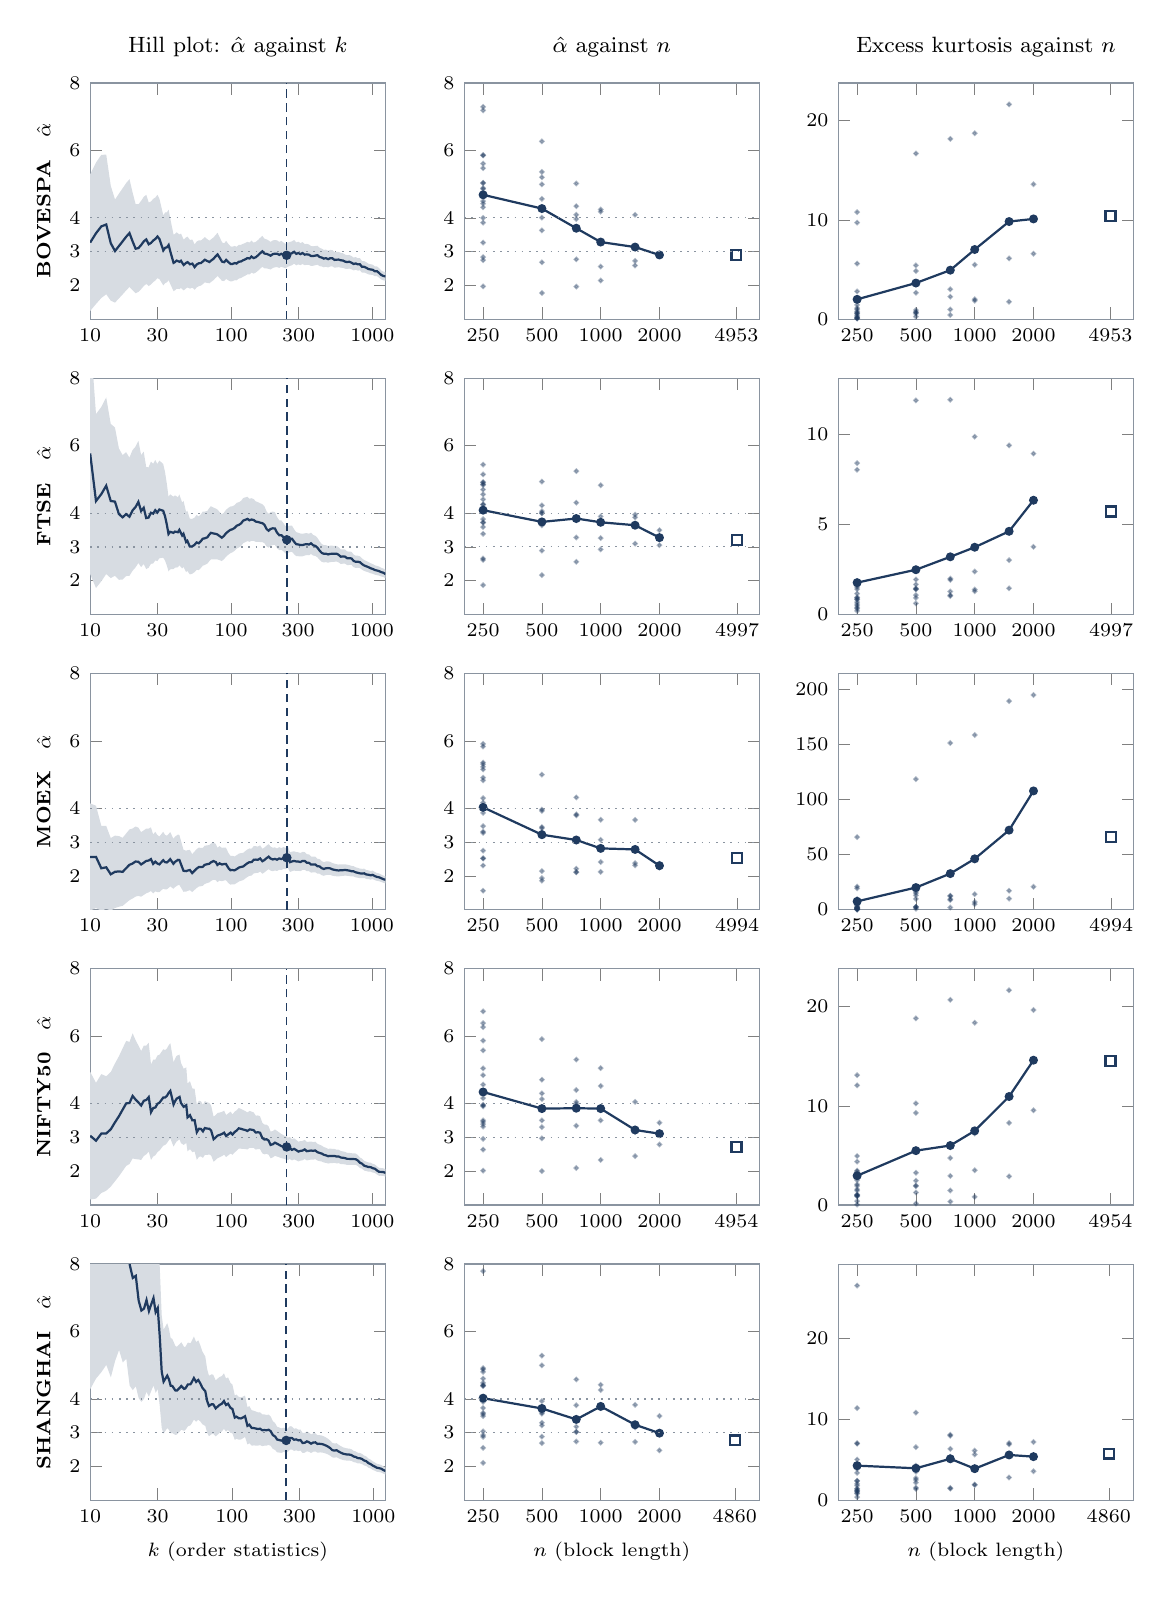
\begin{tikzpicture}
\begin{groupplot}[group style={group size=3 by 5, horizontal sep=1.0cm, vertical sep=0.75cm, x descriptions at=edge bottom}, width=3.75cm, height=3.0cm, scale only axis, tick label style={font=\scriptsize}, label style={font=\scriptsize}, title style={font=\footnotesize}, every axis plot/.append style={line width=0.6pt}, axis line style={draw=Rule}, clip mode=individual]
\nextgroupplot[xmode=log, xmin=10, xmax=1238, ymin=1, ymax=8, ytick={2,3,4,6,8}, xtick={10,30,100,300,1000}, xticklabels={10,30,100,300,1000}, minor tick num=0, ylabel={\textbf{BOVESPA}\quad$\hat\alpha$}, title={Hill plot: $\hat\alpha$ against $k$}]
\addplot[name path=loBOVESPA, draw=none, forget plot] coordinates {(10,1.2432) (11,1.4505) (12,1.628) (13,1.7369) (14,1.5475) (15,1.4912) (16,1.6159) (17,1.7355) (18,1.8524) (19,1.9545) (20,1.8553) (21,1.7673) (22,1.8088) (23,1.8923) (24,1.9837) (25,2.0458) (26,1.982) (27,2.0301) (28,2.0974) (29,2.1491) (30,2.2156) (31,2.1863) (33,2.0013) (34,2.0682) (35,2.0921) (36,2.1539) (37,2.0376) (39,1.8309) (40,1.8585) (41,1.8987) (43,1.8935) (44,1.9242) (46,1.8526) (48,1.9162) (49,1.9376) (51,1.9058) (53,1.9348) (55,1.8711) (57,1.943) (59,1.979) (61,1.9951) (63,2.0425) (65,2.0896) (67,2.0772) (70,2.0627) (72,2.1044) (75,2.1595) (77,2.2129) (80,2.2782) (83,2.2086) (86,2.1339) (89,2.1303) (92,2.1935) (95,2.1547) (99,2.1165) (102,2.1254) (106,2.156) (109,2.151) (113,2.2028) (117,2.2186) (121,2.254) (126,2.2909) (130,2.3265) (135,2.3253) (139,2.3811) (144,2.351) (149,2.379) (155,2.438) (160,2.4934) (166,2.552) (172,2.5043) (178,2.5028) (184,2.491) (190,2.4713) (197,2.5172) (204,2.5379) (211,2.5432) (219,2.5199) (226,2.5549) (234,2.5305) (243,2.5073) (247,2.532) (251,2.5497) (260,2.5758) (269,2.5996) (279,2.645) (289,2.597) (299,2.6245) (309,2.6014) (320,2.6358) (332,2.5989) (343,2.6123) (355,2.6094) (368,2.5772) (381,2.5834) (394,2.5986) (408,2.6153) (423,2.5717) (438,2.5616) (453,2.5375) (469,2.5537) (486,2.5315) (503,2.5606) (520,2.5658) (539,2.524) (558,2.5336) (577,2.5411) (598,2.5252) (619,2.522) (641,2.4951) (663,2.4879) (687,2.4998) (711,2.4782) (736,2.4453) (762,2.4633) (789,2.4409) (817,2.4453) (845,2.3775) (875,2.3824) (906,2.3588) (938,2.3265) (971,2.3174) (1006,2.3111) (1041,2.2726) (1078,2.2785) (1116,2.2306) (1155,2.1773) (1196,2.1507) (1238,2.141)};
\addplot[name path=hiBOVESPA, draw=none, forget plot] coordinates {(10,5.2967) (11,5.6417) (12,5.8709) (13,5.8745) (14,4.9524) (15,4.5468) (16,4.7209) (17,4.8805) (18,5.0335) (19,5.1483) (20,4.7502) (21,4.4088) (22,4.4057) (23,4.5081) (24,4.6294) (25,4.6837) (26,4.4571) (27,4.4893) (28,4.5652) (29,4.6087) (30,4.685) (31,4.5618) (33,4.0743) (34,4.1625) (35,4.1652) (36,4.2438) (37,3.9749) (39,3.5059) (40,3.5277) (41,3.5739) (43,3.5079) (44,3.5382) (46,3.3586) (48,3.4281) (49,3.4447) (51,3.3476) (53,3.3604) (55,3.2154) (57,3.3056) (59,3.335) (61,3.332) (63,3.382) (65,3.4319) (67,3.3852) (70,3.3248) (72,3.3687) (75,3.4229) (77,3.4858) (80,3.5569) (83,3.4194) (86,3.2777) (89,3.2477) (92,3.3202) (95,3.2395) (99,3.155) (102,3.149) (106,3.17) (109,3.1453) (113,3.1987) (117,3.2005) (121,3.2315) (126,3.2602) (130,3.2925) (135,3.269) (139,3.3306) (144,3.269) (149,3.2891) (155,3.3491) (160,3.4077) (166,3.4677) (172,3.3843) (178,3.3648) (184,3.3325) (190,3.2907) (197,3.3343) (204,3.3452) (211,3.3366) (219,3.2893) (226,3.321) (234,3.2742) (243,3.2285) (247,3.2536) (251,3.2696) (260,3.2886) (269,3.3052) (279,3.3483) (289,3.2738) (299,3.2955) (309,3.2543) (320,3.2845) (332,3.2254) (343,3.2307) (355,3.2154) (368,3.1638) (381,3.1602) (394,3.168) (408,3.1774) (423,3.1135) (438,3.091) (453,3.0522) (469,3.0619) (486,3.0256) (503,3.051) (520,3.0484) (539,2.9894) (558,2.9921) (577,2.9926) (598,2.9652) (619,2.9534) (641,2.9139) (663,2.8979) (687,2.9039) (711,2.8714) (736,2.8262) (762,2.8398) (789,2.8071) (817,2.8053) (845,2.7213) (875,2.7205) (906,2.6874) (938,2.6446) (971,2.6285) (1006,2.6155) (1041,2.5665) (1078,2.5678) (1116,2.5087) (1155,2.4439) (1196,2.4091) (1238,2.3936)};
\addplot[Accent!18, forget plot] fill between[of=loBOVESPA and hiBOVESPA];
\addplot[Rule, dotted, thin, forget plot] coordinates {(10,3) (1238,3)};
\addplot[Rule, dotted, thin, forget plot] coordinates {(10,4) (1238,4)};
\addplot[Accent, thick, forget plot] coordinates {(10,3.2699) (11,3.5461) (12,3.7495) (13,3.8057) (14,3.25) (15,3.019) (16,3.1684) (17,3.308) (18,3.443) (19,3.5514) (20,3.3027) (21,3.088) (22,3.1072) (23,3.2002) (24,3.3066) (25,3.3648) (26,3.2196) (27,3.2597) (28,3.3313) (29,3.3789) (30,3.4503) (31,3.3741) (33,3.0378) (34,3.1153) (35,3.1286) (36,3.1989) (37,3.0063) (39,2.6684) (40,2.6931) (41,2.7363) (43,2.7007) (44,2.7312) (46,2.6056) (48,2.6721) (49,2.6912) (51,2.6267) (53,2.6476) (55,2.5432) (57,2.6243) (59,2.657) (61,2.6635) (63,2.7122) (65,2.7607) (67,2.7312) (70,2.6937) (72,2.7365) (75,2.7912) (77,2.8494) (80,2.9175) (83,2.814) (86,2.7058) (89,2.689) (92,2.7569) (95,2.6971) (99,2.6357) (102,2.6372) (106,2.663) (109,2.6481) (113,2.7007) (117,2.7095) (121,2.7427) (126,2.7755) (130,2.8095) (135,2.7971) (139,2.8558) (144,2.81) (149,2.834) (155,2.8936) (160,2.9506) (166,3.0098) (172,2.9443) (178,2.9338) (184,2.9117) (190,2.881) (197,2.9258) (204,2.9416) (211,2.9399) (219,2.9046) (226,2.938) (234,2.9023) (243,2.8679) (247,2.8928) (251,2.9096) (260,2.9322) (269,2.9524) (279,2.9966) (289,2.9354) (299,2.96) (309,2.9279) (320,2.9602) (332,2.9122) (343,2.9215) (355,2.9124) (368,2.8705) (381,2.8718) (394,2.8833) (408,2.8963) (423,2.8426) (438,2.8263) (453,2.7948) (469,2.8078) (486,2.7786) (503,2.8058) (520,2.8071) (539,2.7567) (558,2.7629) (577,2.7668) (598,2.7452) (619,2.7377) (641,2.7045) (663,2.6929) (687,2.7019) (711,2.6748) (736,2.6357) (762,2.6515) (789,2.624) (817,2.6253) (845,2.5494) (875,2.5515) (906,2.5231) (938,2.4855) (971,2.4729) (1006,2.4633) (1041,2.4195) (1078,2.4232) (1116,2.3696) (1155,2.3106) (1196,2.2799) (1238,2.2673)};
\addplot[densely dashed, Accent, forget plot] coordinates {(247,1) (247,8)};
\addplot[only marks, mark=*, mark size=1.4pt, Accent, forget plot] coordinates {(247,2.8928)};
\nextgroupplot[xmode=log, xmin=200, xmax=6500, xtick={250,500,1000,2000,4953}, xticklabels={250,500,1000,2000,4953}, minor tick num=0, ymin=1, ymax=8, ytick={2,3,4,6,8}, title={$\hat\alpha$ against $n$}]
\addplot[only marks, mark=*, mark size=0.7pt, Accent, opacity=0.35, forget plot] coordinates {(250,4.8586) (250,4.4956) (250,3.8597) (250,4.3164) (250,2.7475) (250,7.2939) (250,5.6103) (250,5.859) (250,5.8568) (250,5.4733) (250,2.8414) (250,4.4233) (250,7.1871) (250,1.9717) (250,5.0325) (250,4.0001) (250,4.8851) (250,5.042) (250,3.2705) (500,4.9958) (500,2.6858) (500,4.0097) (500,5.2052) (500,6.2694) (500,3.6307) (500,1.7753) (500,4.5672) (500,5.3637) (750,2.773) (750,4.3493) (750,3.9696) (750,4.0921) (750,1.9646) (750,5.0202) (1000,2.559) (1000,4.2515) (1000,4.1858) (1000,2.145) (1500,2.7273) (1500,4.0931) (1500,2.5903) (2000,2.912) (2000,2.8942)};
\addplot[Accent, thick, mark=*, mark size=1.2pt, forget plot] coordinates {(250,4.6855) (500,4.2781) (750,3.6948) (1000,3.2853) (1500,3.1369) (2000,2.9031)};
\addplot[only marks, mark=square, mark size=1.8pt, Accent, thick, forget plot] coordinates {(4953,2.8928)};
\addplot[Rule, dotted, thin, forget plot] coordinates {(200,3) (6500,3)};
\addplot[Rule, dotted, thin, forget plot] coordinates {(200,4) (6500,4)};
\nextgroupplot[xmode=log, xmin=200, xmax=6500, xtick={250,500,1000,2000,4953}, xticklabels={250,500,1000,2000,4953}, minor tick num=0, ymin=0, title={Excess kurtosis against $n$}]
\addplot[only marks, mark=*, mark size=0.7pt, Accent, opacity=0.35, forget plot] coordinates {(250,1.9732) (250,0.22765) (250,2.7924) (250,1.4463) (250,5.6027) (250,-0.032162) (250,0.36599) (250,0.11983) (250,0.13802) (250,0.98737) (250,9.7229) (250,0.52795) (250,0.59567) (250,10.776) (250,0.65127) (250,0.77949) (250,0.099223) (250,0.04972) (250,1.1233) (500,0.92112) (500,5.4193) (500,2.6606) (500,0.25348) (500,0.56257) (500,4.8514) (500,16.681) (500,0.71667) (500,0.69316) (750,4.7839) (750,2.268) (750,0.42267) (750,3.0143) (750,18.154) (750,0.97963) (1000,5.4781) (1000,1.8586) (1000,1.9998) (1000,18.724) (1500,6.1185) (1500,1.755) (1500,21.623) (2000,6.598) (2000,13.59)};
\addplot[Accent, thick, mark=*, mark size=1.2pt, forget plot] coordinates {(250,1.9972) (500,3.64) (750,4.937) (1000,7.015) (1500,9.8321) (2000,10.094)};
\addplot[only marks, mark=square, mark size=1.8pt, Accent, thick, forget plot] coordinates {(4953,10.355)};
\nextgroupplot[xmode=log, xmin=10, xmax=1249, ymin=1, ymax=8, ytick={2,3,4,6,8}, xtick={10,30,100,300,1000}, xticklabels={10,30,100,300,1000}, minor tick num=0, ylabel={\textbf{FTSE}\quad$\hat\alpha$}]
\addplot[name path=loFTSE, draw=none, forget plot] coordinates {(10,2.1946) (11,1.7839) (12,1.9826) (13,2.1975) (14,2.0771) (15,2.1453) (16,2.0266) (17,2.0346) (18,2.1374) (19,2.1437) (20,2.2933) (21,2.3938) (22,2.5237) (23,2.4021) (24,2.496) (25,2.3445) (26,2.3832) (27,2.4999) (28,2.51) (29,2.6011) (30,2.5817) (31,2.6638) (33,2.6828) (34,2.597) (35,2.4542) (36,2.2777) (37,2.3374) (39,2.3446) (40,2.3849) (42,2.3968) (43,2.4588) (45,2.3626) (46,2.4099) (48,2.2559) (49,2.2898) (51,2.1854) (53,2.2056) (55,2.2504) (57,2.3209) (59,2.3157) (61,2.3722) (63,2.4434) (65,2.4635) (68,2.5058) (70,2.5741) (72,2.6283) (75,2.6305) (78,2.6346) (80,2.6319) (83,2.6082) (86,2.5829) (89,2.6323) (92,2.7064) (96,2.7734) (99,2.816) (102,2.8379) (106,2.8834) (110,2.9522) (114,2.9846) (118,3.0323) (122,3.1084) (126,3.1386) (131,3.1754) (135,3.1505) (140,3.181) (145,3.1796) (150,3.1504) (155,3.1523) (161,3.146) (167,3.1433) (173,3.1098) (179,3.0139) (185,2.9787) (191,3.0322) (198,3.0572) (205,3.0619) (212,2.9671) (220,2.9061) (228,2.914) (236,2.8667) (244,2.8081) (249,2.8132) (253,2.8236) (262,2.8474) (271,2.8581) (281,2.7834) (290,2.7294) (301,2.725) (311,2.719) (322,2.7221) (334,2.7457) (346,2.7582) (358,2.7538) (370,2.7909) (383,2.7456) (397,2.7334) (411,2.6909) (426,2.6161) (441,2.5598) (456,2.5415) (472,2.5494) (489,2.5321) (506,2.5511) (524,2.5575) (543,2.5613) (562,2.568) (582,2.5401) (602,2.4943) (624,2.5049) (646,2.5034) (668,2.4629) (692,2.4655) (717,2.4661) (742,2.4019) (768,2.3785) (795,2.3844) (823,2.3745) (852,2.3252) (883,2.2888) (914,2.2688) (946,2.2476) (979,2.2211) (1014,2.2044) (1050,2.1776) (1087,2.1648) (1125,2.1513) (1165,2.1248) (1206,2.1108) (1249,2.0735)};
\addplot[name path=hiFTSE, draw=none, forget plot] coordinates {(10,9.3502) (11,6.9385) (12,7.1498) (13,7.4323) (14,6.6473) (15,6.5412) (16,5.921) (17,5.7218) (18,5.808) (19,5.6466) (20,5.8718) (21,5.9718) (22,6.147) (23,5.7226) (24,5.8252) (25,5.3677) (26,5.3594) (27,5.5281) (28,5.4634) (29,5.5779) (30,5.4591) (31,5.5581) (33,5.4617) (34,5.227) (35,4.8859) (36,4.4878) (37,4.5598) (39,4.4895) (40,4.5268) (42,4.4752) (43,4.5552) (45,4.3132) (46,4.3688) (48,4.0358) (49,4.0707) (51,3.8387) (53,3.8308) (55,3.8672) (57,3.9486) (59,3.9023) (61,3.9618) (63,4.0459) (65,4.046) (68,4.0683) (70,4.1491) (72,4.2072) (75,4.1696) (78,4.1376) (80,4.1091) (83,4.0381) (86,3.9673) (89,4.0129) (92,4.0965) (96,4.1605) (99,4.1976) (102,4.2047) (106,4.2394) (110,4.3093) (114,4.3268) (118,4.3674) (122,4.4495) (126,4.4666) (131,4.4877) (135,4.4291) (140,4.4442) (145,4.4159) (150,4.3508) (155,4.3303) (161,4.2955) (167,4.2672) (173,4.1989) (179,4.0485) (185,3.9818) (191,4.0344) (198,4.0467) (205,4.0331) (212,3.8901) (220,3.791) (228,3.7833) (236,3.7052) (244,3.6139) (249,3.6112) (253,3.6173) (262,3.632) (271,3.6306) (281,3.5205) (290,3.4394) (301,3.4191) (311,3.399) (322,3.3897) (334,3.4053) (346,3.4079) (358,3.3903) (370,3.4242) (383,3.3567) (397,3.3299) (411,3.2669) (426,3.1651) (441,3.0868) (456,3.0552) (472,3.055) (489,3.0246) (506,3.0381) (524,3.0365) (543,3.0317) (562,3.0309) (582,2.9894) (602,2.9274) (624,2.9315) (646,2.9217) (668,2.8671) (692,2.8625) (717,2.8557) (742,2.7743) (768,2.7406) (795,2.7406) (823,2.7227) (852,2.66) (883,2.6121) (914,2.5834) (946,2.5536) (979,2.518) (1014,2.4935) (1050,2.458) (1087,2.4384) (1125,2.4183) (1165,2.3837) (1206,2.3633) (1249,2.317)};
\addplot[Accent!18, forget plot] fill between[of=loFTSE and hiFTSE];
\addplot[Rule, dotted, thin, forget plot] coordinates {(10,3) (1249,3)};
\addplot[Rule, dotted, thin, forget plot] coordinates {(10,4) (1249,4)};
\addplot[Accent, thick, forget plot] coordinates {(10,5.7724) (11,4.3612) (12,4.5662) (13,4.8149) (14,4.3622) (15,4.3432) (16,3.9738) (17,3.8782) (18,3.9727) (19,3.8951) (20,4.0825) (21,4.1828) (22,4.3353) (23,4.0624) (24,4.1606) (25,3.8561) (26,3.8713) (27,4.014) (28,3.9867) (29,4.0895) (30,4.0204) (31,4.1109) (33,4.0722) (34,3.912) (35,3.6701) (36,3.3828) (37,3.4486) (39,3.4171) (40,3.4558) (42,3.436) (43,3.507) (45,3.3379) (46,3.3894) (48,3.1459) (49,3.1802) (51,3.012) (53,3.0182) (55,3.0588) (57,3.1347) (59,3.109) (61,3.167) (63,3.2446) (65,3.2547) (68,3.2871) (70,3.3616) (72,3.4178) (75,3.4) (78,3.3861) (80,3.3705) (83,3.3232) (86,3.2751) (89,3.3226) (92,3.4015) (96,3.4669) (99,3.5068) (102,3.5213) (106,3.5614) (110,3.6307) (114,3.6557) (118,3.6999) (122,3.779) (126,3.8026) (131,3.8316) (135,3.7898) (140,3.8126) (145,3.7978) (150,3.7506) (155,3.7413) (161,3.7208) (167,3.7052) (173,3.6544) (179,3.5312) (185,3.4803) (191,3.5333) (198,3.552) (205,3.5475) (212,3.4286) (220,3.3486) (228,3.3486) (236,3.286) (244,3.211) (249,3.2122) (253,3.2205) (262,3.2397) (271,3.2443) (281,3.1519) (290,3.0844) (301,3.072) (311,3.059) (322,3.0559) (334,3.0755) (346,3.0831) (358,3.0721) (370,3.1076) (383,3.0512) (397,3.0316) (411,2.9789) (426,2.8906) (441,2.8233) (456,2.7983) (472,2.8022) (489,2.7783) (506,2.7946) (524,2.797) (543,2.7965) (562,2.7994) (582,2.7648) (602,2.7108) (624,2.7182) (646,2.7126) (668,2.665) (692,2.664) (717,2.6609) (742,2.5881) (768,2.5595) (795,2.5625) (823,2.5486) (852,2.4926) (883,2.4504) (914,2.4261) (946,2.4006) (979,2.3695) (1014,2.349) (1050,2.3178) (1087,2.3016) (1125,2.2848) (1165,2.2542) (1206,2.237) (1249,2.1953)};
\addplot[densely dashed, Accent, forget plot] coordinates {(249,1) (249,8)};
\addplot[only marks, mark=*, mark size=1.4pt, Accent, forget plot] coordinates {(249,3.2122)};
\nextgroupplot[xmode=log, xmin=200, xmax=6500, xtick={250,500,1000,2000,4997}, xticklabels={250,500,1000,2000,4997}, minor tick num=0, ymin=1, ymax=8, ytick={2,3,4,6,8}]
\addplot[only marks, mark=*, mark size=0.7pt, Accent, opacity=0.35, forget plot] coordinates {(250,4.4099) (250,4.2557) (250,5.1478) (250,4.5602) (250,2.6578) (250,4.702) (250,4.2639) (250,3.7288) (250,3.7206) (250,4.9245) (250,4.9088) (250,3.5906) (250,4.8531) (250,1.8668) (250,5.4385) (250,4.8414) (250,3.8257) (250,3.3897) (250,2.6136) (500,3.64) (500,2.8912) (500,4.0014) (500,4.9378) (500,4.0003) (500,4.0588) (500,2.167) (500,4.2306) (500,3.7547) (750,3.2816) (750,4.3126) (750,3.7942) (750,5.2472) (750,2.5588) (750,3.8591) (1000,3.2626) (1000,3.9042) (1000,4.8289) (1000,2.9276) (1500,3.8756) (1500,3.9581) (1500,3.0968) (2000,3.4982) (2000,3.0534)};
\addplot[Accent, thick, mark=*, mark size=1.2pt, forget plot] coordinates {(250,4.0894) (500,3.7424) (750,3.8422) (1000,3.7308) (1500,3.6435) (2000,3.2758)};
\addplot[only marks, mark=square, mark size=1.8pt, Accent, thick, forget plot] coordinates {(4997,3.2122)};
\addplot[Rule, dotted, thin, forget plot] coordinates {(200,3) (6500,3)};
\addplot[Rule, dotted, thin, forget plot] coordinates {(200,4) (6500,4)};
\nextgroupplot[xmode=log, xmin=200, xmax=6500, xtick={250,500,1000,2000,4997}, xticklabels={250,500,1000,2000,4997}, minor tick num=0, ymin=0]
\addplot[only marks, mark=*, mark size=0.7pt, Accent, opacity=0.35, forget plot] coordinates {(250,1.6976) (250,0.92019) (250,0.48372) (250,0.85558) (250,0.95034) (250,1.1623) (250,1.4029) (250,0.68056) (250,1.7436) (250,0.3269) (250,0.19771) (250,1.8582) (250,0.82102) (250,8.4187) (250,0.37649) (250,0.57371) (250,1.5973) (250,1.5225) (250,8.0488) (500,1.4087) (500,1.9448) (500,1.0768) (500,1.4499) (500,0.92344) (500,1.402) (500,11.907) (500,0.61258) (500,1.6678) (750,1.9944) (750,1.0276) (750,1.9227) (750,1.0722) (750,11.946) (750,1.2758) (1000,2.3862) (1000,1.3865) (1000,1.2928) (1000,9.8894) (1500,3.0178) (1500,1.4554) (1500,9.4024) (2000,3.7603) (2000,8.9467)};
\addplot[Accent, thick, mark=*, mark size=1.2pt, forget plot] coordinates {(250,1.7704) (500,2.4881) (750,3.2064) (1000,3.7387) (1500,4.6252) (2000,6.3535)};
\addplot[only marks, mark=square, mark size=1.8pt, Accent, thick, forget plot] coordinates {(4997,5.7245)};
\nextgroupplot[xmode=log, xmin=10, xmax=1248, ymin=1, ymax=8, ytick={2,3,4,6,8}, xtick={10,30,100,300,1000}, xticklabels={10,30,100,300,1000}, minor tick num=0, ylabel={\textbf{MOEX}\quad$\hat\alpha$}]
\addplot[name path=loMOEX, draw=none, forget plot] coordinates {(10,0.97372) (11,1.0494) (12,0.96692) (13,1.0301) (14,0.97587) (15,1.0482) (16,1.089) (17,1.1129) (18,1.1992) (19,1.2821) (20,1.3304) (21,1.3891) (22,1.4091) (23,1.3843) (24,1.4354) (25,1.4868) (26,1.5125) (27,1.5568) (28,1.4841) (29,1.5424) (30,1.5208) (31,1.5183) (33,1.625) (34,1.5992) (35,1.6048) (36,1.6433) (37,1.6929) (39,1.6198) (40,1.667) (42,1.7285) (43,1.7336) (45,1.5973) (46,1.5311) (48,1.5365) (49,1.5533) (51,1.5792) (53,1.524) (55,1.5832) (57,1.6422) (59,1.6853) (61,1.6962) (63,1.7087) (65,1.7626) (68,1.7917) (70,1.8074) (72,1.8487) (75,1.8893) (78,1.8756) (80,1.8171) (83,1.8635) (86,1.8442) (89,1.8635) (92,1.8754) (96,1.7835) (99,1.7431) (102,1.7537) (106,1.7538) (110,1.7944) (114,1.8377) (118,1.8588) (122,1.8756) (126,1.9211) (131,1.9721) (135,2.0027) (140,2.0105) (145,2.076) (150,2.0874) (155,2.0888) (161,2.1294) (167,2.066) (172,2.0986) (179,2.159) (185,2.2015) (191,2.1586) (198,2.1422) (205,2.1623) (212,2.1481) (220,2.1859) (228,2.1762) (236,2.2092) (244,2.2005) (249,2.2249) (253,2.2487) (262,2.1182) (271,2.1415) (280,2.1589) (290,2.1508) (301,2.1515) (311,2.144) (322,2.179) (334,2.1825) (345,2.1411) (358,2.141) (370,2.0995) (383,2.105) (397,2.1099) (411,2.0664) (425,2.0667) (440,2.0235) (456,2.0045) (472,2.0272) (489,2.0359) (506,2.0309) (524,2.0079) (542,1.9979) (562,1.9897) (581,1.9869) (602,1.9975) (623,2.0007) (645,2.0101) (668,2.005) (692,1.9974) (716,1.9846) (741,1.9841) (768,1.9581) (795,1.9478) (823,1.9349) (852,1.933) (882,1.9405) (913,1.9106) (945,1.9067) (979,1.8923) (1013,1.9068) (1049,1.876) (1086,1.8544) (1125,1.8461) (1164,1.8219) (1205,1.7975) (1248,1.7824)};
\addplot[name path=hiMOEX, draw=none, forget plot] coordinates {(10,4.1485) (11,4.0818) (12,3.4869) (13,3.484) (14,3.123) (15,3.196) (16,3.1815) (17,3.1298) (18,3.2585) (19,3.3772) (20,3.4063) (21,3.4655) (22,3.4321) (23,3.2979) (24,3.35) (25,3.404) (26,3.4013) (27,3.4425) (28,3.2303) (29,3.3077) (30,3.2157) (31,3.168) (33,3.3081) (34,3.2186) (35,3.195) (36,3.2379) (37,3.3026) (39,3.1016) (40,3.1643) (42,3.2272) (43,3.2117) (45,2.9159) (46,2.7756) (48,2.7488) (49,2.7614) (51,2.7739) (53,2.6469) (55,2.7207) (57,2.7939) (59,2.84) (61,2.8328) (63,2.8293) (65,2.8949) (68,2.909) (70,2.9133) (72,2.9593) (75,2.9946) (78,2.9455) (80,2.837) (83,2.885) (86,2.8327) (89,2.8409) (92,2.8388) (96,2.6755) (99,2.5983) (102,2.5983) (106,2.5785) (110,2.6192) (114,2.6642) (118,2.6773) (122,2.6848) (126,2.7339) (131,2.7872) (135,2.8154) (140,2.8088) (145,2.8832) (150,2.8828) (155,2.8694) (161,2.9074) (167,2.8047) (172,2.8361) (179,2.9001) (185,2.9428) (191,2.8721) (198,2.8355) (205,2.8482) (212,2.8163) (220,2.8516) (228,2.8254) (236,2.8553) (244,2.8319) (249,2.856) (253,2.8808) (262,2.7018) (271,2.7204) (280,2.7318) (290,2.7103) (301,2.6996) (311,2.6802) (322,2.7134) (334,2.7069) (345,2.6462) (358,2.6358) (370,2.5759) (383,2.5736) (397,2.5703) (411,2.5087) (425,2.501) (440,2.4407) (456,2.4096) (472,2.4293) (489,2.4319) (506,2.4187) (524,2.384) (542,2.3652) (562,2.3483) (581,2.3386) (602,2.3443) (623,2.3416) (645,2.3464) (668,2.3341) (692,2.319) (716,2.2983) (741,2.2919) (768,2.2561) (795,2.2388) (823,2.2187) (852,2.2112) (882,2.2148) (913,2.1757) (945,2.1664) (979,2.1453) (1013,2.157) (1049,2.1176) (1086,2.0889) (1125,2.0752) (1164,2.044) (1205,2.0126) (1248,1.9918)};
\addplot[Accent!18, forget plot] fill between[of=loMOEX and hiMOEX];
\addplot[Rule, dotted, thin, forget plot] coordinates {(10,3) (1248,3)};
\addplot[Rule, dotted, thin, forget plot] coordinates {(10,4) (1248,4)};
\addplot[Accent, thick, forget plot] coordinates {(10,2.5611) (11,2.5656) (12,2.2269) (13,2.257) (14,2.0494) (15,2.1221) (16,2.1352) (17,2.1214) (18,2.2288) (19,2.3296) (20,2.3683) (21,2.4273) (22,2.4206) (23,2.3411) (24,2.3927) (25,2.4454) (26,2.4569) (27,2.4997) (28,2.3572) (29,2.425) (30,2.3682) (31,2.3432) (33,2.4666) (34,2.4089) (35,2.3999) (36,2.4406) (37,2.4978) (39,2.3607) (40,2.4157) (42,2.4778) (43,2.4726) (45,2.2566) (46,2.1533) (48,2.1426) (49,2.1574) (51,2.1765) (53,2.0855) (55,2.152) (57,2.218) (59,2.2626) (61,2.2645) (63,2.269) (65,2.3288) (68,2.3503) (70,2.3603) (72,2.404) (75,2.4419) (78,2.4105) (80,2.327) (83,2.3743) (86,2.3385) (89,2.3522) (92,2.3571) (96,2.2295) (99,2.1707) (102,2.176) (106,2.1661) (110,2.2068) (114,2.251) (118,2.268) (122,2.2802) (126,2.3275) (131,2.3797) (135,2.409) (140,2.4097) (145,2.4796) (150,2.4851) (155,2.4791) (161,2.5184) (167,2.4353) (172,2.4674) (179,2.5295) (185,2.5722) (191,2.5154) (198,2.4889) (205,2.5053) (212,2.4822) (220,2.5188) (228,2.5008) (236,2.5322) (244,2.5162) (249,2.5405) (253,2.5648) (262,2.41) (271,2.431) (280,2.4453) (290,2.4306) (301,2.4256) (311,2.4121) (322,2.4462) (334,2.4447) (345,2.3936) (358,2.3884) (370,2.3377) (383,2.3393) (397,2.3401) (411,2.2875) (425,2.2838) (440,2.2321) (456,2.207) (472,2.2283) (489,2.2339) (506,2.2248) (524,2.196) (542,2.1816) (562,2.169) (581,2.1628) (602,2.1709) (623,2.1711) (645,2.1783) (668,2.1696) (692,2.1582) (716,2.1415) (741,2.138) (768,2.1071) (795,2.0933) (823,2.0768) (852,2.0721) (882,2.0777) (913,2.0431) (945,2.0366) (979,2.0188) (1013,2.0319) (1049,1.9968) (1086,1.9717) (1125,1.9606) (1164,1.933) (1205,1.905) (1248,1.8871)};
\addplot[densely dashed, Accent, forget plot] coordinates {(249,1) (249,8)};
\addplot[only marks, mark=*, mark size=1.4pt, Accent, forget plot] coordinates {(249,2.5405)};
\nextgroupplot[xmode=log, xmin=200, xmax=6500, xtick={250,500,1000,2000,4994}, xticklabels={250,500,1000,2000,4994}, minor tick num=0, ymin=1, ymax=8, ytick={2,3,4,6,8}]
\addplot[only marks, mark=*, mark size=0.7pt, Accent, opacity=0.35, forget plot] coordinates {(250,4.9117) (250,3.8696) (250,2.3089) (250,5.8355) (250,2.7485) (250,5.9157) (250,5.3103) (250,2.5222) (250,5.3615) (250,4.3041) (250,4.8322) (250,3.4751) (250,5.1554) (250,2.5202) (250,4.1732) (250,1.5617) (250,3.3123) (250,5.2357) (250,3.2766) (500,3.9687) (500,2.1444) (500,3.4499) (500,3.4148) (500,3.9273) (500,3.3007) (500,1.8585) (500,1.9347) (500,5.0038) (750,2.107) (750,4.3278) (750,3.8252) (750,3.7953) (750,2.2162) (750,2.1188) (1000,2.4118) (1000,3.0711) (1000,3.6639) (1000,2.1206) (1500,2.382) (1500,3.6606) (1500,2.3154) (2000,2.3622) (2000,2.2464)};
\addplot[Accent, thick, mark=*, mark size=1.2pt, forget plot] coordinates {(250,4.0332) (500,3.2225) (750,3.0651) (1000,2.8168) (1500,2.786) (2000,2.3043)};
\addplot[only marks, mark=square, mark size=1.8pt, Accent, thick, forget plot] coordinates {(4994,2.5405)};
\addplot[Rule, dotted, thin, forget plot] coordinates {(200,3) (6500,3)};
\addplot[Rule, dotted, thin, forget plot] coordinates {(200,4) (6500,4)};
\nextgroupplot[xmode=log, xmin=200, xmax=6500, xtick={250,500,1000,2000,4994}, xticklabels={250,500,1000,2000,4994}, minor tick num=0, ymin=0]
\addplot[only marks, mark=*, mark size=0.7pt, Accent, opacity=0.35, forget plot] coordinates {(250,1.63) (250,2.4116) (250,5.2497) (250,1.0864) (250,4.4741) (250,1.1184) (250,0.92274) (250,19.437) (250,0.39362) (250,1.4826) (250,0.24067) (250,21.041) (250,0.058657) (250,9.5789) (250,0.72225) (250,65.899) (250,2.1843) (250,2.4405) (250,3.7053) (500,2.5) (500,9.8151) (500,2.5785) (500,16.397) (500,0.86938) (500,15.104) (500,13.029) (500,118.35) (500,2.3385) (750,12.661) (750,1.9978) (750,9.598) (750,8.8693) (750,12.351) (750,151.08) (1000,14.101) (1000,7.0136) (1000,5.0564) (1000,158.39) (1500,17.222) (1500,10.045) (1500,189.15) (2000,20.738) (2000,194.67)};
\addplot[Accent, thick, mark=*, mark size=1.2pt, forget plot] coordinates {(250,7.583) (500,20.109) (750,32.76) (1000,46.141) (1500,72.14) (2000,107.7)};
\addplot[only marks, mark=square, mark size=1.8pt, Accent, thick, forget plot] coordinates {(4994,65.633)};
\nextgroupplot[xmode=log, xmin=10, xmax=1238, ymin=1, ymax=8, ytick={2,3,4,6,8}, xtick={10,30,100,300,1000}, xticklabels={10,30,100,300,1000}, minor tick num=0, ylabel={\textbf{NIFTY50}\quad$\hat\alpha$}]
\addplot[name path=loNIFTY50, draw=none, forget plot] coordinates {(10,1.1609) (11,1.1879) (12,1.3526) (13,1.4238) (14,1.5439) (15,1.7038) (16,1.8516) (17,2.0069) (18,2.1575) (19,2.2132) (20,2.3772) (21,2.3577) (22,2.3497) (23,2.3343) (24,2.4523) (25,2.4998) (26,2.5828) (27,2.3352) (28,2.4383) (29,2.4741) (30,2.5676) (31,2.6127) (33,2.7573) (34,2.7785) (35,2.831) (36,2.9099) (37,2.9695) (39,2.7303) (40,2.8132) (41,2.8794) (43,2.9459) (44,2.8343) (46,2.7792) (48,2.8373) (49,2.5886) (51,2.656) (53,2.5636) (55,2.5856) (57,2.3366) (59,2.4266) (61,2.4375) (63,2.3965) (65,2.4829) (67,2.4837) (70,2.4944) (72,2.4663) (75,2.2806) (77,2.3206) (80,2.3867) (83,2.4157) (86,2.4482) (89,2.489) (92,2.4212) (95,2.4686) (99,2.5252) (102,2.487) (106,2.5638) (109,2.6009) (113,2.6684) (117,2.6673) (121,2.6612) (126,2.6574) (130,2.6434) (135,2.6929) (139,2.6938) (144,2.6925) (149,2.6405) (155,2.6583) (160,2.6538) (166,2.5308) (172,2.5002) (178,2.5144) (184,2.4879) (190,2.3839) (197,2.4086) (204,2.4567) (211,2.4356) (219,2.4115) (226,2.3886) (234,2.3747) (243,2.3503) (247,2.3803) (251,2.3305) (260,2.3638) (269,2.3188) (279,2.3499) (289,2.3224) (299,2.2896) (309,2.3126) (320,2.3243) (332,2.3619) (343,2.3194) (355,2.3322) (368,2.346) (381,2.3416) (394,2.3574) (408,2.315) (423,2.3002) (438,2.2865) (453,2.258) (469,2.2469) (486,2.2278) (503,2.2401) (520,2.242) (539,2.2461) (558,2.2325) (577,2.2387) (598,2.2123) (619,2.2099) (641,2.2026) (663,2.1859) (687,2.1886) (711,2.1862) (736,2.1892) (762,2.1897) (789,2.1563) (817,2.0967) (845,2.0756) (875,2.0198) (906,2.0049) (938,1.9878) (971,1.9877) (1006,1.9601) (1041,1.9498) (1078,1.9037) (1116,1.8653) (1155,1.8663) (1196,1.863) (1238,1.8414)};
\addplot[name path=hiNIFTY50, draw=none, forget plot] coordinates {(10,4.9458) (11,4.6204) (12,4.8778) (13,4.8154) (14,4.9408) (15,5.1953) (16,5.4095) (17,5.6438) (18,5.8626) (19,5.8296) (20,6.0868) (21,5.8819) (22,5.7231) (23,5.561) (24,5.7231) (25,5.7232) (26,5.8081) (27,5.1638) (28,5.3073) (29,5.3057) (30,5.4293) (31,5.4516) (33,5.6133) (34,5.5921) (35,5.6362) (36,5.7334) (37,5.7929) (39,5.228) (40,5.3399) (41,5.4198) (43,5.4577) (44,5.2117) (46,5.0384) (48,5.0759) (49,4.602) (51,4.6654) (53,4.4526) (55,4.4432) (57,3.9751) (59,4.0893) (61,4.0707) (63,3.9681) (65,4.0779) (67,4.0477) (70,4.0207) (72,3.9479) (75,3.6149) (77,3.6554) (80,3.7262) (83,3.7401) (86,3.7604) (89,3.7945) (92,3.6649) (95,3.7114) (99,3.7642) (102,3.6848) (106,3.7694) (109,3.8031) (113,3.8748) (117,3.8479) (121,3.8152) (126,3.7818) (130,3.7409) (135,3.7858) (139,3.768) (144,3.7438) (149,3.6507) (155,3.6516) (160,3.627) (166,3.439) (172,3.3788) (178,3.3804) (184,3.3283) (190,3.1743) (197,3.1905) (204,3.2382) (211,3.1955) (219,3.1478) (226,3.1048) (234,3.0727) (243,3.0263) (247,3.0586) (251,2.9885) (260,3.0179) (269,2.9483) (279,2.9747) (289,2.9277) (299,2.875) (309,2.893) (320,2.8963) (332,2.9313) (343,2.8684) (355,2.8737) (368,2.88) (381,2.8644) (394,2.874) (408,2.8125) (423,2.7848) (438,2.759) (453,2.716) (469,2.6941) (486,2.6626) (503,2.6691) (520,2.6636) (539,2.6603) (558,2.6364) (577,2.6365) (598,2.5979) (619,2.5879) (641,2.5722) (663,2.5461) (687,2.5424) (711,2.5331) (736,2.5302) (762,2.5244) (789,2.4798) (817,2.4054) (845,2.3757) (875,2.3065) (906,2.2842) (938,2.2597) (971,2.2545) (1006,2.2183) (1041,2.202) (1078,2.1454) (1116,2.0978) (1155,2.0947) (1196,2.0868) (1238,2.0586)};
\addplot[Accent!18, forget plot] fill between[of=loNIFTY50 and hiNIFTY50];
\addplot[Rule, dotted, thin, forget plot] coordinates {(10,3) (1238,3)};
\addplot[Rule, dotted, thin, forget plot] coordinates {(10,4) (1238,4)};
\addplot[Accent, thick, forget plot] coordinates {(10,3.0533) (11,2.9042) (12,3.1152) (13,3.1196) (14,3.2423) (15,3.4496) (16,3.6305) (17,3.8253) (18,4.01) (19,4.0214) (20,4.232) (21,4.1198) (22,4.0364) (23,3.9476) (24,4.0877) (25,4.1115) (26,4.1954) (27,3.7495) (28,3.8728) (29,3.8899) (30,3.9985) (31,4.0322) (33,4.1853) (34,4.1853) (35,4.2336) (36,4.3217) (37,4.3812) (39,3.9791) (40,4.0766) (41,4.1496) (43,4.2018) (44,4.023) (46,3.9088) (48,3.9566) (49,3.5953) (51,3.6607) (53,3.5081) (55,3.5144) (57,3.1559) (59,3.258) (61,3.2541) (63,3.1823) (65,3.2804) (67,3.2657) (70,3.2575) (72,3.2071) (75,2.9477) (77,2.988) (80,3.0564) (83,3.0779) (86,3.1043) (89,3.1418) (92,3.0431) (95,3.09) (99,3.1447) (102,3.0859) (106,3.1666) (109,3.202) (113,3.2716) (117,3.2576) (121,3.2382) (126,3.2196) (130,3.1921) (135,3.2394) (139,3.2309) (144,3.2181) (149,3.1456) (155,3.1549) (160,3.1404) (166,2.9849) (172,2.9395) (178,2.9474) (184,2.9081) (190,2.7791) (197,2.7995) (204,2.8474) (211,2.8155) (219,2.7797) (226,2.7467) (234,2.7237) (243,2.6883) (247,2.7194) (251,2.6595) (260,2.6908) (269,2.6336) (279,2.6623) (289,2.625) (299,2.5823) (309,2.6028) (320,2.6103) (332,2.6466) (343,2.5939) (355,2.6029) (368,2.613) (381,2.603) (394,2.6157) (408,2.5638) (423,2.5425) (438,2.5228) (453,2.487) (469,2.4705) (486,2.4452) (503,2.4546) (520,2.4528) (539,2.4532) (558,2.4344) (577,2.4376) (598,2.4051) (619,2.3989) (641,2.3874) (663,2.366) (687,2.3655) (711,2.3596) (736,2.3597) (762,2.3571) (789,2.3181) (817,2.2511) (845,2.2256) (875,2.1632) (906,2.1446) (938,2.1237) (971,2.1211) (1006,2.0892) (1041,2.0759) (1078,2.0245) (1116,1.9816) (1155,1.9805) (1196,1.9749) (1238,1.95)};
\addplot[densely dashed, Accent, forget plot] coordinates {(247,1) (247,8)};
\addplot[only marks, mark=*, mark size=1.4pt, Accent, forget plot] coordinates {(247,2.7194)};
\nextgroupplot[xmode=log, xmin=200, xmax=6500, xtick={250,500,1000,2000,4954}, xticklabels={250,500,1000,2000,4954}, minor tick num=0, ymin=1, ymax=8, ytick={2,3,4,6,8}]
\addplot[only marks, mark=*, mark size=0.7pt, Accent, opacity=0.35, forget plot] coordinates {(250,3.9205) (250,5.8697) (250,3.3966) (250,4.5667) (250,6.3877) (250,6.7376) (250,3.9547) (250,6.2678) (250,3.9642) (250,4.1643) (250,5.0495) (250,3.4605) (250,3.3232) (250,2.0158) (250,2.9591) (250,4.8443) (250,5.5807) (250,2.6425) (250,3.5057) (500,4.7109) (500,2.9753) (500,5.9153) (500,4.1388) (500,4.3052) (500,3.3056) (500,2.0037) (500,3.8418) (500,3.5053) (750,3.9924) (750,5.3081) (750,4.0535) (750,4.4055) (750,2.0946) (750,3.3461) (1000,3.5062) (1000,5.0552) (1000,4.5263) (1000,2.334) (1500,3.1644) (1500,4.0543) (1500,2.4467) (2000,3.434) (2000,2.7913)};
\addplot[Accent, thick, mark=*, mark size=1.2pt, forget plot] coordinates {(250,4.348) (500,3.8558) (750,3.8667) (1000,3.8554) (1500,3.2218) (2000,3.1126)};
\addplot[only marks, mark=square, mark size=1.8pt, Accent, thick, forget plot] coordinates {(4954,2.7194)};
\addplot[Rule, dotted, thin, forget plot] coordinates {(200,3) (6500,3)};
\addplot[Rule, dotted, thin, forget plot] coordinates {(200,4) (6500,4)};
\nextgroupplot[xmode=log, xmin=200, xmax=6500, xtick={250,500,1000,2000,4954}, xticklabels={250,500,1000,2000,4954}, minor tick num=0, ymin=0]
\addplot[only marks, mark=*, mark size=0.7pt, Accent, opacity=0.35, forget plot] coordinates {(250,1.9265) (250,1.4556) (250,4.9414) (250,0.8659) (250,-0.089032) (250,0.38058) (250,2.0789) (250,0.9394) (250,4.3761) (250,1.0466) (250,1.5898) (250,0.9564) (250,3.4773) (250,13.089) (250,3.3752) (250,1.0252) (250,0.04854) (250,12.076) (250,2.5111) (500,2.4514) (500,9.2887) (500,0.15055) (500,1.9025) (500,3.2518) (500,1.2623) (500,18.828) (500,1.9558) (500,10.246) (750,5.8294) (750,0.33976) (750,2.9324) (750,1.4682) (750,20.693) (750,4.7341) (1000,7.213) (1000,0.8185) (1000,3.5053) (1000,18.386) (1500,8.279) (1500,2.8851) (1500,21.66) (2000,9.5469) (2000,19.666)};
\addplot[Accent, thick, mark=*, mark size=1.2pt, forget plot] coordinates {(250,2.9511) (500,5.4819) (750,5.9995) (1000,7.4807) (1500,10.942) (2000,14.606)};
\addplot[only marks, mark=square, mark size=1.8pt, Accent, thick, forget plot] coordinates {(4954,14.525)};
\nextgroupplot[xmode=log, xmin=10, xmax=1215, ymin=1, ymax=8, ytick={2,3,4,6,8}, xtick={10,30,100,300,1000}, xticklabels={10,30,100,300,1000}, minor tick num=0, ylabel={\textbf{SHANGHAI}\quad$\hat\alpha$}, xlabel={$k$ (order statistics)}]
\addplot[name path=loSHANGHAI, draw=none, forget plot] coordinates {(10,4.2874) (11,4.6052) (12,4.7952) (13,5.0123) (14,4.6411) (15,5.1276) (16,5.4506) (17,5.082) (18,5.194) (19,4.3973) (20,4.2623) (21,4.378) (22,4.026) (23,3.9158) (24,4.0064) (25,4.2144) (26,4.0668) (27,4.2402) (28,4.4023) (29,4.1807) (30,4.2998) (31,3.7918) (32,3.1449) (33,2.9742) (35,3.138) (36,3.0868) (37,2.9779) (38,2.9928) (40,2.9334) (41,2.9481) (43,3.0409) (44,3.0908) (46,3.0586) (47,3.0795) (49,3.1914) (51,3.2177) (52,3.269) (54,3.388) (56,3.3263) (58,3.3893) (60,3.3308) (62,3.253) (65,3.2016) (67,2.9967) (69,2.8987) (72,2.9564) (74,2.9663) (77,2.8903) (79,2.9357) (82,2.9977) (85,3.0379) (88,3.1167) (91,3.0369) (94,3.0803) (98,2.9966) (101,2.9823) (105,2.7895) (108,2.8206) (112,2.7937) (116,2.8016) (120,2.8355) (124,2.8749) (129,2.6519) (133,2.6884) (138,2.6189) (143,2.6234) (148,2.6211) (153,2.618) (158,2.6344) (164,2.6045) (170,2.617) (176,2.6193) (182,2.6401) (188,2.6132) (195,2.5188) (202,2.492) (209,2.418) (216,2.4135) (224,2.4039) (232,2.4315) (240,2.4244) (242,2.4233) (248,2.431) (257,2.4984) (266,2.5016) (275,2.4631) (285,2.4778) (295,2.4574) (305,2.4726) (316,2.4) (327,2.4091) (339,2.452) (350,2.4359) (363,2.4011) (376,2.4378) (389,2.4461) (402,2.4086) (417,2.416) (431,2.4146) (446,2.4032) (462,2.3814) (478,2.3567) (495,2.3217) (512,2.2703) (530,2.2608) (549,2.2749) (568,2.2417) (588,2.2155) (609,2.1918) (630,2.1818) (653,2.1738) (676,2.1753) (699,2.1659) (724,2.1302) (749,2.1195) (776,2.0906) (803,2.0893) (831,2.0705) (860,2.0317) (890,2.0163) (922,1.9638) (954,1.942) (988,1.9015) (1022,1.875) (1058,1.8445) (1095,1.8349) (1134,1.8225) (1174,1.7873) (1215,1.7624)};
\addplot[name path=hiSHANGHAI, draw=none, forget plot] coordinates {(10,18.267) (11,17.912) (12,17.293) (13,16.952) (14,14.852) (15,15.635) (16,15.924) (17,14.292) (18,14.114) (19,11.583) (20,10.913) (21,10.922) (22,9.8061) (23,9.3286) (24,9.3501) (25,9.6488) (26,9.1454) (27,9.3764) (28,9.5823) (29,8.9654) (30,9.092) (31,7.9118) (32,6.4797) (33,6.0549) (35,6.2474) (36,6.082) (37,5.8092) (38,5.7831) (40,5.5681) (41,5.5492) (43,5.6337) (44,5.6835) (46,5.545) (47,5.5454) (49,5.6737) (51,5.652) (52,5.7093) (54,5.8527) (56,5.687) (58,5.7384) (60,5.5875) (62,5.4091) (65,5.2582) (67,4.8836) (69,4.689) (72,4.7325) (74,4.7168) (77,4.5528) (79,4.5968) (82,4.6538) (85,4.6782) (88,4.7631) (91,4.6076) (94,4.6413) (98,4.4762) (101,4.4274) (105,4.109) (108,4.1318) (112,4.0637) (116,4.0481) (120,4.0714) (124,4.1031) (129,3.758) (133,3.7893) (138,3.6678) (143,3.652) (148,3.6279) (153,3.6039) (158,3.6077) (164,3.5458) (170,3.543) (176,3.5274) (182,3.5377) (188,3.485) (195,3.3414) (202,3.2893) (209,3.1765) (216,3.1563) (224,3.1284) (232,3.1497) (240,3.1267) (242,3.1219) (248,3.1221) (257,3.1944) (266,3.185) (275,3.1233) (285,3.1288) (295,3.0905) (305,3.0978) (316,2.9948) (327,2.9948) (339,3.0363) (350,3.006) (363,2.9518) (376,2.9861) (389,2.9859) (402,2.9305) (417,2.929) (431,2.9181) (446,2.8949) (462,2.8593) (478,2.8209) (495,2.7703) (512,2.7009) (530,2.6816) (549,2.6903) (568,2.6435) (588,2.6051) (609,2.57) (630,2.5514) (653,2.535) (676,2.53) (699,2.5127) (724,2.465) (749,2.4465) (776,2.4071) (803,2.3998) (831,2.3726) (860,2.3228) (890,2.2999) (922,2.2348) (954,2.2052) (988,2.1544) (1022,2.1199) (1058,2.081) (1095,2.0659) (1134,2.0477) (1174,2.0041) (1215,1.9724)};
\addplot[Accent!18, forget plot] fill between[of=loSHANGHAI and hiSHANGHAI];
\addplot[Rule, dotted, thin, forget plot] coordinates {(10,3) (1215,3)};
\addplot[Rule, dotted, thin, forget plot] coordinates {(10,4) (1215,4)};
\addplot[Accent, thick, forget plot] coordinates {(10,11.277) (11,11.259) (12,11.044) (13,10.982) (14,9.7468) (15,10.381) (16,10.687) (17,9.6869) (18,9.6539) (19,7.9901) (20,7.5878) (21,7.6499) (22,6.9161) (23,6.6222) (24,6.6782) (25,6.9316) (26,6.6061) (27,6.8083) (28,6.9923) (29,6.5731) (30,6.6959) (31,5.8518) (32,4.8123) (33,4.5145) (35,4.6927) (36,4.5844) (37,4.3936) (38,4.3879) (40,4.2508) (41,4.2487) (43,4.3373) (44,4.3872) (46,4.3018) (47,4.3125) (49,4.4326) (51,4.4349) (52,4.4891) (54,4.6203) (56,4.5067) (58,4.5639) (60,4.4592) (62,4.331) (65,4.2299) (67,3.9401) (69,3.7939) (72,3.8445) (74,3.8415) (77,3.7216) (79,3.7662) (82,3.8257) (85,3.858) (88,3.9399) (91,3.8223) (94,3.8608) (98,3.7364) (101,3.7048) (105,3.4492) (108,3.4762) (112,3.4287) (116,3.4249) (120,3.4535) (124,3.489) (129,3.2049) (133,3.2388) (138,3.1434) (143,3.1377) (148,3.1245) (153,3.1109) (158,3.1211) (164,3.0752) (170,3.08) (176,3.0734) (182,3.0889) (188,3.0491) (195,2.9301) (202,2.8907) (209,2.7972) (216,2.7849) (224,2.7662) (232,2.7906) (240,2.7755) (242,2.7726) (248,2.7765) (257,2.8464) (266,2.8433) (275,2.7932) (285,2.8033) (295,2.7739) (305,2.7852) (316,2.6974) (327,2.702) (339,2.7442) (350,2.721) (363,2.6764) (376,2.712) (389,2.716) (402,2.6696) (417,2.6725) (431,2.6664) (446,2.6491) (462,2.6204) (478,2.5888) (495,2.546) (512,2.4856) (530,2.4712) (549,2.4826) (568,2.4426) (588,2.4103) (609,2.3809) (630,2.3666) (653,2.3544) (676,2.3527) (699,2.3393) (724,2.2976) (749,2.283) (776,2.2488) (803,2.2445) (831,2.2216) (860,2.1773) (890,2.1581) (922,2.0993) (954,2.0736) (988,2.0279) (1022,1.9974) (1058,1.9628) (1095,1.9504) (1134,1.9351) (1174,1.8957) (1215,1.8674)};
\addplot[densely dashed, Accent, forget plot] coordinates {(242,1) (242,8)};
\addplot[only marks, mark=*, mark size=1.4pt, Accent, forget plot] coordinates {(242,2.7726)};
\nextgroupplot[xmode=log, xmin=200, xmax=6500, xtick={250,500,1000,2000,4860}, xticklabels={250,500,1000,2000,4860}, minor tick num=0, ymin=1, ymax=8, ytick={2,3,4,6,8}, xlabel={$n$ (block length)}]
\addplot[only marks, mark=*, mark size=0.7pt, Accent, opacity=0.35, forget plot] coordinates {(250,3.7333) (250,4.3845) (250,3.589) (250,3.9124) (250,4.8058) (250,4.4135) (250,4.4759) (250,4.8756) (250,4.6021) (250,2.5534) (250,3.0422) (250,3.5534) (250,3.4936) (250,2.1072) (250,7.7897) (250,4.3975) (250,4.9121) (250,2.8792) (250,2.9282) (500,3.9366) (500,3.2153) (500,4.9959) (500,3.5632) (500,3.2964) (500,3.6042) (500,2.6931) (500,5.2832) (500,2.8848) (750,3.8153) (750,4.5804) (750,2.7403) (750,3.0191) (750,3.032) (750,3.1796) (1000,4.2664) (1000,4.4198) (1000,2.7048) (1000,3.7298) (1500,3.8272) (1500,2.7287) (1500,3.1564) (2000,3.4967) (2000,2.4771)};
\addplot[Accent, thick, mark=*, mark size=1.2pt, forget plot] coordinates {(250,4.0236) (500,3.7192) (750,3.3944) (1000,3.7802) (1500,3.2375) (2000,2.9869)};
\addplot[only marks, mark=square, mark size=1.8pt, Accent, thick, forget plot] coordinates {(4860,2.7726)};
\addplot[Rule, dotted, thin, forget plot] coordinates {(200,3) (6500,3)};
\addplot[Rule, dotted, thin, forget plot] coordinates {(200,4) (6500,4)};
\nextgroupplot[xmode=log, xmin=200, xmax=6500, xtick={250,500,1000,2000,4860}, xticklabels={250,500,1000,2000,4860}, minor tick num=0, ymin=0, xlabel={$n$ (block length)}]
\addplot[only marks, mark=*, mark size=0.7pt, Accent, opacity=0.35, forget plot] coordinates {(250,3.8756) (250,0.92901) (250,1.3727) (250,1.1598) (250,1.4509) (250,1.0862) (250,2.4104) (250,0.82892) (250,1.8106) (250,6.9945) (250,2.3928) (250,2.0374) (250,5.0441) (250,7.0654) (250,0.38867) (250,3.3913) (250,1.1895) (250,11.414) (250,26.571) (500,1.5618) (500,2.1866) (500,1.3993) (500,2.5218) (500,3.5263) (500,4.2801) (500,6.5681) (500,2.7415) (500,10.837) (750,1.5201) (750,1.4447) (750,5.384) (750,8.108) (750,6.3584) (750,7.9914) (1000,1.9419) (1000,1.8954) (1000,6.146) (1000,5.6618) (1500,2.8179) (1500,6.9209) (1500,7.0787) (2000,3.5892) (2000,7.2083)};
\addplot[Accent, thick, mark=*, mark size=1.2pt, forget plot] coordinates {(250,4.2849) (500,3.958) (750,5.1344) (1000,3.9113) (1500,5.6059) (2000,5.3987)};
\addplot[only marks, mark=square, mark size=1.8pt, Accent, thick, forget plot] coordinates {(4860,5.7746)};
\end{groupplot}
\end{tikzpicture}
\caption{Hill plots and sample-size dependence, one row per market, full series 2006--2026. \emph{Left:} $\hat\alpha$ against the number of order statistics $k$ (log axis). The band is $\hat\alpha(1\pm1.96/\sqrt{k})$, the asymptotic band for i.i.d.\ data, which understates the uncertainty under volatility clustering. The dashed line and dot mark the top 5\,\% used by \texttt{tail\_index\_diff} and Table~\ref{tab:data}; dotted lines mark $\alpha=3$ and $\alpha=4$, below which skewness and kurtosis do not exist. \emph{Centre and right:} top-5\,\% $\hat\alpha$ and sample excess kurtosis on disjoint blocks of $n$ days. Dots are single blocks, the line is their mean, the square is the whole series (Table~\ref{tab:data}'s value). The left and centre vertical axes are common to all rows; the right one is free. Values above the axis limit are clipped: SHANGHAI's curve leaves the axis for $k\le18$ ($11.3$ at $k=10$).}
\label{fig:hill}
\end{figure}

\paragraph{Why both ARCH-LM variants are descriptive-only} \texttt{arch\_pvalue\_diff} identifies the better-fitting model $99\%$ of the time on simulated GARCH but saturates completely on real data: real and shuffled both underflow to $p=0.0$, giving $|\Delta p|=0.000000$ and rating the adversarial control a perfect match. \texttt{arch\_stat\_diff} scores $76\%$ with a null sd of $46.4$ --- two draws from the same process gave LM $56.8$ and $124.8$. Neither is reliable across both regimes. ACF-MAE replaces them as the primary volatility-clustering signal: continuous, no saturation, $88\%$ Monte Carlo accuracy.

\paragraph{Why the discriminative AUC was ranked on $|\text{AUC}-0.5|$, and why it no longer is} \textit{Evidence for the original choice:} under an ascending rank on the raw value, an anti-predictive AUC of $0.30$ outranked an indistinguishable $0.50$, because the optimum is $0.5$, not $0$. The rank on $|\text{AUC}-0.5|$ assumed a real-versus-real null of $0.5$, which the corrected null contradicts (Section~\ref{sec:walkforward}); a second ranked column, a $z$-score against a null, depended on how that null was built. Both columns left the ranked set at S4 (Section~\ref{sec:s4}).

\paragraph{Why downstream utility uses conditional VaR} Unconditional VaR was tested first and added nothing: Gaussian iid noise scored identically to real data (coverage error 0.0276 for both), because an unconditional quantile probes only the marginal --- already covered by Wasserstein and the quantile MSE. Conditional VaR probes whether the GARCH structure itself transfers, which is the question TSTR is asking.

\paragraph{Why QLIKE needs a large $n$, and what that means here} QLIKE inverts at small samples: at $n\approx126$ Gaussian noise scored $-6.888$ against real data's $-6.876$, ranking noise above real. At $n=623$ pooled it ranks correctly with sd $0.000$. The pipeline therefore computes it once per seed over every market's concatenated test set: $n$ is 2,479 here (Table~\ref{tab:downstream}), which meets the $n\gtrsim600$ threshold, at the disclosed cost of the variance filter crossing 4 market boundaries.

\paragraph{Why Gaussian QMLE for the residual-kurtosis metric} A Student-$t$ specification absorbs excess kurtosis by construction and makes the test uninformative for every model. Gaussian QMLE keeps it able to fail. Circularity with the GARCH generators is discussed in Results.

\paragraph{Why determinism is not enforced} \texttt{torch.use\_deterministic\_algorithms(True)} and \texttt{cudnn.deterministic} are deliberately unset; the cost is measured rather than assumed (Section~\ref{sec:results}). Consequence, stated as a rule: no single-run winner is reported on \texttt{tail\_index\_diff}, \texttt{hurst\_diff} or \texttt{mean\_diff}, because those three change their winner between identical repeat runs.

\paragraph{Instrumentation retained} The \texttt{[DIAG]} latent statistics, the \texttt{[WARNING]} post-generation guard and the step-count printout are kept in the pipeline permanently. Each fires rarely; between them they located latent collapse, mode collapse and the $492\times$ budget gap. The guard's firings in this run are a reported result (Section~\ref{sec:results}), not a debug artefact.
\subsection{Methods added in this version}
\label{sec:newmethods}
Four methods enter the pipeline or the audit in this version. Each is stated with the measurement that motivated it, and each measurement is an artifact of this repository.

\paragraph{S4: the discriminative AUC leaves the ranked set}\label{sec:s4} The decision was taken on the following grounds, before its effect on the ranking was known. \textit{(i) Neither column has a working reference.} $|\mathrm{AUC}-0.5|$ assumes a real-versus-real null of $0.5$; the null on these series has mean 0.57--0.69 at the fixed-split length (Table~\ref{tab:nulls}). $|\mathrm{AUC}-\mu_0|/\sigma_0$ reads a null that rests on about 5 independent block pairs drawn from 20 years of history, and its construction moved first and second place when it was changed. \textit{(ii) The correct estimator does not repair them.} Purged and embargoed cross-validation (below) leaves the anti-predictive draws where they were, so they are regime drift, not leakage (Section~\ref{sec:walkforward}). \textit{(iii) The value is set by the direction of drift, not by generator quality:} the shuffled control's AUC runs 0.31--0.68 across the five markets under purged folds, and lies below the purged null in four of the five. \textit{(iv) Nothing clears a calibrated threshold} on fresh draws (0 of 25 cells, Section~\ref{sec:walkforward}). \textit{(v) Method choice is small next to generation noise:} a fresh generation draw moves 53 of 75 within-unit positions, a change of AUC calibration or cross-validation scheme moves 6 to 13, and dropping the two columns (S4) moves 23 (all measured before the scaler fix; Section~\ref{sec:scaler}). \texttt{TEMPORAL\_COLS} is now five metrics, the two AUC columns are in \texttt{DESCRIPTIVE\_COLS}, and the comment beside them in the notebook records these grounds.

\paragraph{Purged and embargoed cross-validation, as an option}\label{sec:purged} \texttt{compute\_discriminative\_score(cv='purged')} keeps the folds contiguous and drops, on both sides of each test chunk, the training windows within one window length (20) of it, so no observation is shared between a training row and a test row. At five folds it drops 40 / 80 / 80 / 80 / 40 training rows per fold (5--11\,\% of the training rows at the fixed-split length, 3--6\,\% at walk-forward length); the smallest training set is 665 rows, so the folds remain large enough to fit. The default is unchanged (contiguous, as published); shuffled folds are refused. Both schemes are computed for every null (Table~\ref{tab:nulls}).

\paragraph{The scaler fix}\label{sec:scaler} The discriminative metric standardised its features on all rows before the folds were cut, so the test fold's mean and scale entered the training features under every scheme, purged included. The scaler is now a step of a scikit-learn \texttt{Pipeline} and is fitted within each training fold. Measured on the same pairs before and after: the null means and standard deviations move by at most 0.008, individual AUC values by up to 0.18 in a few series in strongly drifting stretches (0.018 on the published draw), and no count in Section~\ref{sec:walkforward} changes. The cached AUC nulls now carry the scaler convention in their key, so pre-fix caches are recomputed rather than reused.

\paragraph{Fair baselines, and their confinement to the training block}\label{sec:baseline-methods} Two trivial generators with no access to the test block were added as comparison entries; they never enter the composite. \emph{I.i.d.\ historical simulation} resamples returns with replacement from the training block; it is the standard industry baseline for value-at-risk. The \emph{stationary block bootstrap} (Politis \& Romano) resamples geometric-length blocks, circularly, inside the training block, with the mean block length chosen by the Politis--White rule (\texttt{arch} 8.0.0). Applied to raw returns the rule returns 0.27--5.43 (one market below one observation, floored at one), because raw returns lack linear autocorrelation, so that bootstrap is nearly i.i.d.; applied to $|r|$ it returns 111--128, the scale of volatility persistence, which is the specification that matters for the temporal metrics and is the one called the block-bootstrap baseline in the text. Table~\ref{tab:pw} gives both. Each baseline is drawn 20 times per market--seed and scored through the same \texttt{FinancialMetrics} code path as the generators; the generators' and control's rows reproduced from that path equal the stored Phase~B rows exactly. \emph{Confinement:} the generating functions receive the training array, a length and a random generator and nothing else; the validation file is not opened, and from the test file only the row count is taken, from the parquet footer. Of 900 stored draws, 0 contain a value that is not in the training block, every index used lies below the training length, and regenerating from the recorded seeds reproduces every draw.

\begin{table}[htbp]
\centering
\caption{The two bootstraps, per market: training length, target length, and the Politis--White mean block length on the returns and on $|r|$, then the lengths used (the returns-based length floored at one observation).}
\label{tab:pw}
\begin{tabular}{@{}lrrrrrr@{}}
\toprule
Market & Train & Target & PW, $r$ & PW, $|r|$ & Used, $r$ & Used, $|r|$ \\
\midrule
BOVESPA & 3,962 & 496 & 5.43 & 111.4 & 5.43 & 111.4 \\
FTSE & 3,997 & 501 & 0.27 & 122.9 & 1.00 & 122.9 \\
MOEX & 3,995 & 500 & 2.19 & 125.7 & 2.19 & 125.7 \\
NIFTY50 & 3,963 & 496 & 2.57 & 122.1 & 2.57 & 122.1 \\
SHANGHAI & 3,888 & 486 & 1.69 & 127.9 & 1.69 & 127.9 \\
\bottomrule
\end{tabular}
\end{table}

%% ─── Architecture comparison ─────────────────────────────────────────────────
\section{Architecture comparison}
\label{sec:architecture}
The benchmark compares five generators in two families. The three \emph{gradient-trained} models are generative adversarial networks trained on windows of 128 consecutive returns to an asserted parity of 9,000 generator updates: TimeGAN\tcite{4}, a recurrent autoencoder with an adversarial latent model; QuantGAN\tcite{5}, a temporal convolutional network trained as a Wasserstein GAN with gradient penalty (WGAN-GP)\tcite{3}; and CNN-WGAN-GP, a transposed-convolution generator trained with the same objective. The CNN-WGAN-GP is named for its architecture and is distinct from the published Fin-GAN\tcite{41}, which forecasts and classifies returns with an economics-driven loss; this one is an unconditional generator and makes no forecasts. The two \emph{econometric} models, GARCH(1,1)\tcite{39} and GJR-GARCH(1,1)\tcite{40} with Student-$t$ innovations, are fitted by maximum likelihood on the market's raw returns. Table~\ref{tab:architecture} sets them side by side.

\begin{table}[htbp]
\centering
\caption{The five generators. Budget parity binds the three gradient-trained models; maximum-likelihood fits have no gradient-step analogue and are exempt.}
\label{tab:architecture}
{\footnotesize\setlength{\tabcolsep}{3.5pt}
\begin{tabularx}{\linewidth}{@{}>{\raggedright\arraybackslash}p{1.85cm}*{5}{>{\raggedright\arraybackslash}X}@{}}
\toprule
 & \textbf{TimeGAN} & \textbf{QuantGAN} & \textbf{CNN-WGAN-GP} & \textbf{GARCH(1,1)-$t$} & \textbf{GJR-GARCH-$t$} \\
\midrule
Family & gradient & gradient & gradient & econometric & econometric \\
Core & 4-phase (embedder $+$ supervisor $+$ GAN), GRU backbone & TCN backbone, WGAN-GP & CNN deconvolution, WGAN-GP & Conditional variance, Student-$t$ innovations & GARCH $+$ leverage indicator \\
Temporal mechanism & Recurrent: each step in order, gating what to remember & Dilated causal convolutions: all time scales in one pass & Transposed convolutions: upsample noise to full sequence & $\sigma_t^2=\omega+\alpha r_{t-1}^2+\beta\sigma_{t-1}^2$ & adds $\gamma r_{t-1}^2\mathbb{1}[r_{t-1}<0]$ \\
Fitting & BCE $+$ moment matching, 4 phases & WGAN-GP, $n_\text{critic}=5$, $\lambda_\text{gp}=10$ & WGAN-GP, $n_\text{critic}=5$, $\lambda_\text{gp}=10$ & ML; constrained refit if persistence reaches 1 & ML; constrained refit if persistence reaches 1 \\
Reference & Yoon et al.\ 2019\tcite{4} & Wiese et al.\ 2020\tcite{5} & This work; not Fin-GAN\tcite{41} & Bollerslev 1986\tcite{39} & Glosten et al.\ 1993\tcite{40} \\
Key settings & hidden\_dim 24, layers 3, lr 1e-3 & noise\_dim 100, lr 1e-4, 3 TCN blocks (dil.\ 1/2/4) & base\_channels 64, lr 1e-4, 3$\times$ConvTranspose1d & $p{=}1,q{=}1,o{=}0$, dist $t$, burn-in 500 & $p{=}1,q{=}1,o{=}1$, dist $t$, burn-in 500 \\
Input scaling & z-score $+\tanh(z/3)\to[-1,1]$ & z-score $+\tanh(z/3)\to[-1,1]$ & z-score $+\tanh(z/3)\to[-1,1]$ & Raw returns $\times100$ & Raw returns $\times100$ \\
seq\_len constraint & any & any & divisible by 8 & n/a & n/a \\
Budget & generator-update parity (asserted) & parity & parity & \textbf{exempt} --- ML fit, no step analogue & \textbf{exempt} \\
Inductive bias & Step-by-step ordering; persistence via GRU state & Multi-scale memory; dilations span short and long horizons & Coarse-to-fine hierarchical refinement, borrowed from image GANs & Conditional heteroskedasticity, symmetric response & As GARCH, plus asymmetric response to negative returns (Cont fact 5\tcite{7}) \\
\bottomrule
\end{tabularx}}
\end{table}

\begin{table}[htbp]
\centering
\caption{Size and cost of each model against its composite rank (Table~\ref{tab:ranking}). \emph{Params}: trainable generator parameters for the gradient-trained models, fitted parameters for the econometric ones (GARCH(1,1)-$t$: $\mu,\omega,\alpha,\beta,\nu$; GJR-GARCH adds $\gamma$). \emph{Gen.\ updates}: \texttt{n/a} for maximum-likelihood fits, which have no gradient-step analogue, rather than an invented number. \emph{Fit}: mean wall-clock seconds to train or fit one model, over every market--seed.}
\label{tab:compute}
\begin{tabular}{@{}llrrrc@{}}
\toprule
Model & Family & Params & Gen.\ updates & Fit (s) & Composite \\
\midrule
GJR-GARCH & econometric & 6 & n/a & 0.018 & 2.493 \\
GARCH & econometric & 5 & n/a & 0.023 & 2.923 \\
TimeGAN & gradient & 11,400 & 9,000 & 81.1 & 3.867 \\
CNN-WGAN-GP & gradient & 55,401 & 9,000 & 180.4 & 2.621 \\
QuantGAN & gradient & 276,481 & 9,000 & 481.1 & 3.096 \\
\bottomrule
\end{tabular}
\end{table}

Table~\ref{tab:compute} records the training regime's cost. Sampling cost --- the time a fitted model takes to generate a series --- was not recorded by this run, so it is not reported. Equal generator updates is not equal compute: QuantGAN and CNN-WGAN-GP each take five critic updates per generator update\tcite{3}, and TimeGAN's 3,000 autoencoder and 3,000 supervisor pre-training steps are excluded from parity and reported separately\tcite{4}.

\subsection{Settings shared by the two WGAN-GP models}
\textbf{$n_\text{critic}=5$:} the critic must estimate the Wasserstein distance accurately before the generator uses its gradient; fewer updates leave it under-fitted and the gradient biased. Gulrajani et al.\ (2017)\tcite{3} establish this as a floor and CTBench\tcite{16} and SFAG\tcite{28} fix it identically.

\textbf{$\lambda_\text{gp}=10$:} values below 5 permit Lipschitz violations, invalidating the Kantorovich--Rubinstein duality the training objective rests on. 10 is the standard from Gulrajani et al.\ and has not been improved on.

\textbf{$\beta_1=0$ in Adam:} in adversarial training the correct generator direction reverses each time the critic updates, so momentum accumulates stale direction and pushes the wrong way. $\beta_1=0$ uses the current gradient only.

\textbf{LayerNorm, not BatchNorm, in the CNN-WGAN-GP critic:} the gradient penalty needs the critic's gradient norm at a \emph{single} interpolated point. BatchNorm makes that value depend on the other samples in the batch, corrupting the penalty.

\subsection{TimeGAN's four-phase training}
\textbf{Phase 1 --- autoencoder:} train embedder $e:\mathcal{X}\to\mathcal{H}$ and recovery $\hat r:\mathcal{H}\to\mathcal{X}$ on $\|X-\hat r(e(X))\|^2$.

\textbf{Phase 2 --- supervisor:} train $s:\mathcal{H}\to\hat{\mathcal{H}}$ on $\|H_{t+1}-s(H_t)\|^2$, injecting temporal causality into the latent space.

\textbf{Phase 3 --- joint adversarial:} $z\to G(z)\to s(G(z))\to\hat r(\cdot)\to\tilde X$, with
\begin{align*}
\mathcal{L}_G &= \mathcal{L}_U + 100\sqrt{\mathcal{L}_S} + 100\,\mathcal{L}_V \\
\mathcal{L}_V &= |\mu_H-\mu_{\hat H}| + |\sigma_H-\sigma_{\hat H}|
\end{align*}

\textbf{Phase 4 --- fine-tuning} of the recovery network on generated sequences.

Phases 1--2 are pre-training and are excluded from budget parity; only phase-3 joint steps are counted, matching QuantGAN's and CNN-WGAN-GP's \texttt{train\_steps}. In this run the pre-training budget was 3,000 autoencoder and 3,000 supervisor steps, reported here rather than folded into the parity figure.

%% ─── Pipeline ────────────────────────────────────────────────────────────────
\section{Pipeline}
\label{sec:pipeline}
Figure~\ref{fig:pipeline} shows the pipeline from price files to ranked results. Each stage is described below in the order it runs.

\begin{figure}[p]
\centering
\resizebox{\linewidth}{!}{%
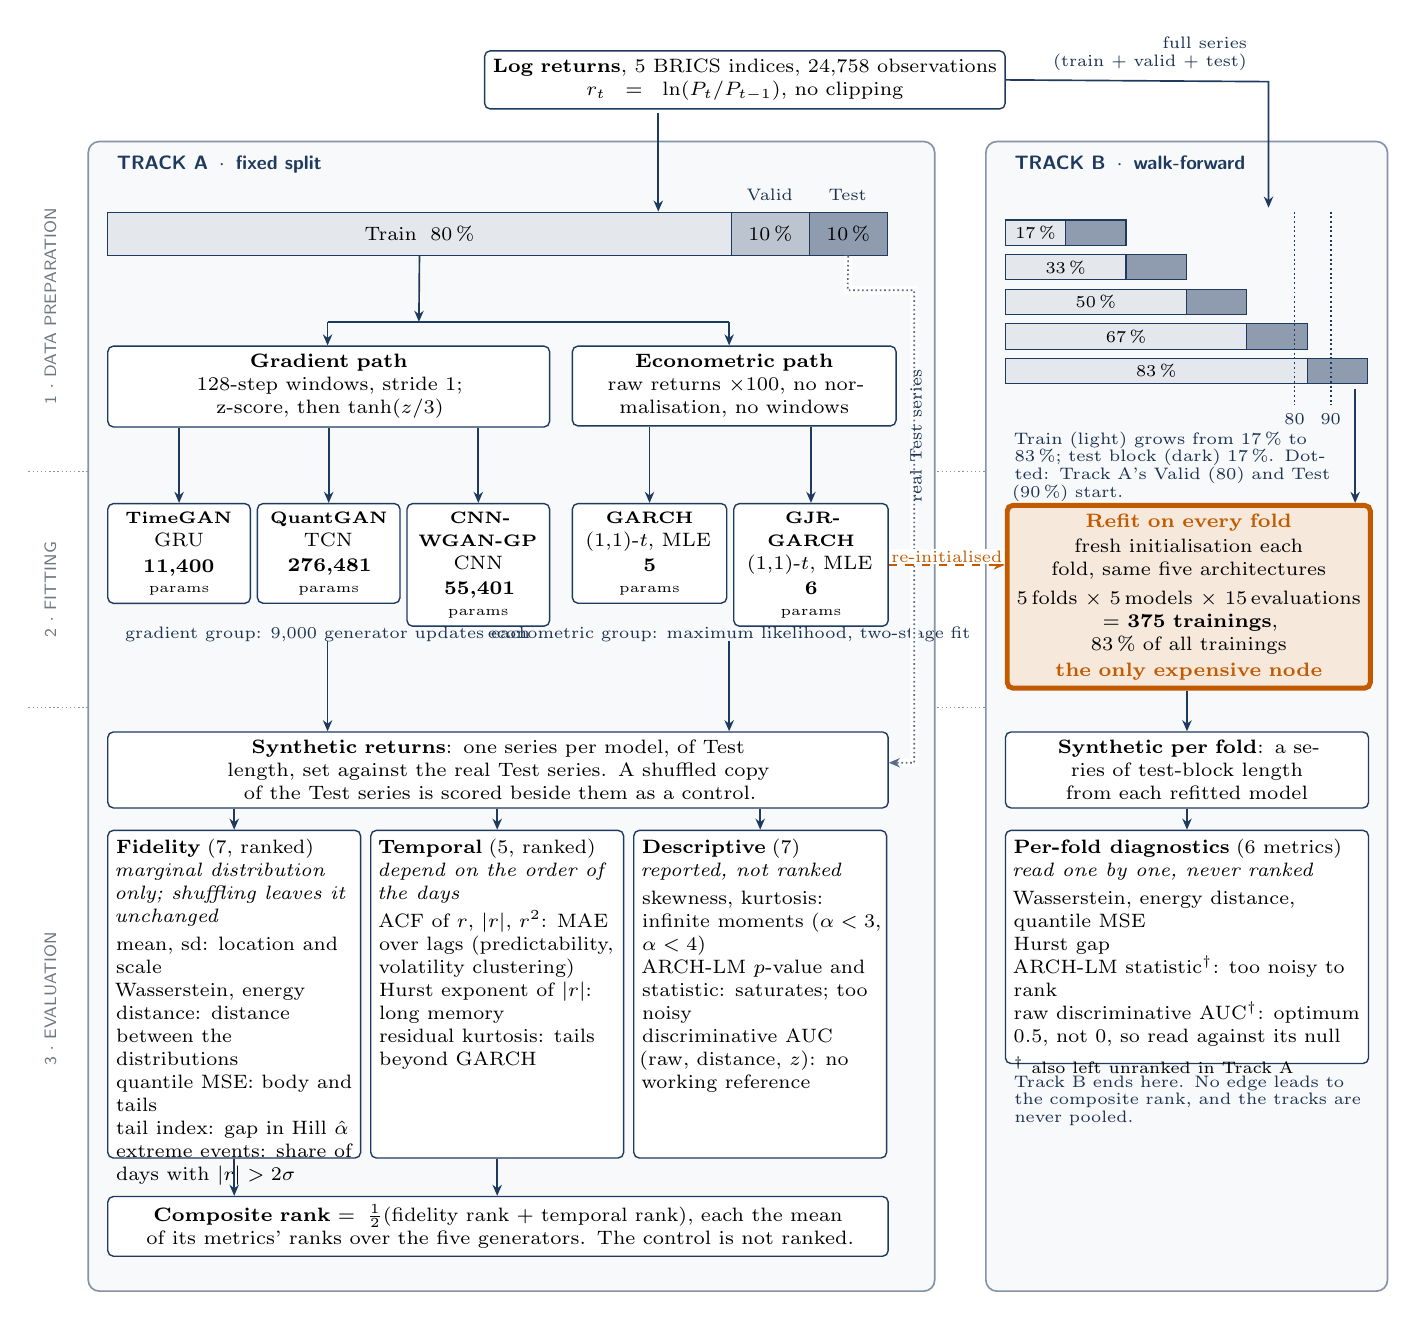
\begin{tikzpicture}[
  x=1cm, y=1cm,
  every node/.style={font=\fontsize{7}{8.3}\selectfont},
  box/.style={rectangle, rounded corners=2pt, draw=Accent, fill=white, line width=0.5pt,
              align=center, inner sep=3pt},
  arr/.style={-{Stealth[length=4pt,width=3.4pt]}, line width=0.6pt, draw=Accent},
  darr/.style={arr, dashed, draw=RefitCol},
  tarr/.style={arr, densely dotted, draw=Accent!75},
  hdr/.style={font=\sffamily\bfseries\fontsize{7.5}{9}\selectfont, text=Accent, anchor=north west},
  stg/.style={font=\sffamily\fontsize{6}{7}\selectfont, text=Rule!80!black, rotate=90},
  tiny/.style={font=\fontsize{5.6}{6.4}\selectfont, text=Accent!85!black},
  seg/.style={draw=Accent, line width=0.4pt, inner sep=0pt, minimum height=0.55cm, align=center},
  rost/.style={box, text width=1.6cm, anchor=north west},
  cont/.style={rectangle, rounded corners=4pt, draw=Accent!55, fill=Accent!3, line width=0.6pt},
]
%% Geometry: Track A occupies x = 0..9.9, Track B x = 11.4..16.0. Stages run
%% top to bottom: 1 data preparation, 2 fitting, 3 evaluation. Both tracks flow
%% downward; nothing runs against that direction.

%% ── Stage separators and labels (drawn first, under everything) ────────────
\draw[Rule, densely dotted, line width=0.5pt] (-1.0,-5.35) -- (16.25,-5.35);
\draw[Rule, densely dotted, line width=0.5pt] (-1.0,-8.35) -- (16.25,-8.35);
\node[stg] at (-0.72,-3.25) {1 $\cdot$ DATA PREPARATION};
\node[stg] at (-0.72,-6.85) {2 $\cdot$ FITTING};
\node[stg] at (-0.72,-12.05) {3 $\cdot$ EVALUATION};

%% ── Track containers ───────────────────────────────────────────────────────
\node[cont, minimum width=10.75cm, minimum height=14.6cm, anchor=north west] at (-0.25,-1.15) {};
\node[cont, minimum width=5.1cm,  minimum height=14.6cm, anchor=north west] at (11.15,-1.15) {};
\node[hdr] at (0,-1.22) {TRACK A \,$\cdot$\, fixed split};
\node[hdr] at (11.4,-1.22) {TRACK B \,$\cdot$\, walk-forward};

%% ── Shared node ────────────────────────────────────────────────────────────
\node[box, text width=6.4cm, anchor=north] (shared) at (8.1,0)
     {\textbf{Log returns}, 5 BRICS indices, 24,758 observations\\$r_t=\ln(P_t/P_{t-1})$, no clipping};

%% ── Track A: the 80 / 10 / 10 split, drawn to scale (width 9.9 = 100 %) ────
\node[seg, fill=Accent!12, minimum width=7.92cm, anchor=north west] (trn) at (0,-2.05) {Train \;80\,\%};
\node[seg, fill=Accent!30, minimum width=0.99cm, anchor=north west] (val) at (7.92,-2.05) {10\,\%};
\node[seg, fill=Accent!50, minimum width=0.99cm, anchor=north west] (tst) at (8.91,-2.05) {10\,\%};
\node[tiny, anchor=south] at (8.415,-2.03) {Valid};
\node[tiny, anchor=south] at (9.405,-2.03) {Test};
\draw[arr] (7.0,-0.8) -- (7.0,-2.05);

%% ── Track B: expanding folds, drawn to scale (width 4.6 = full series) ─────
\draw[arr] (shared.east) -- (14.75,-0.4) -- (14.75,-2.0);
\node[tiny, align=right, anchor=south east] at (14.6,-0.38) {full series\\(train + valid + test)};
\foreach \k in {0,...,4} {
  \pgfmathsetmacro{\yy}{-2.15-0.44*\k}
  \pgfmathsetmacro{\wtr}{4.6*(\k+1)/(5+1)}
  \pgfmathsetmacro{\wte}{4.6/(5+1)}
  \pgfmathtruncatemacro{\pct}{round(100*(\k+1)/(5+1))}
  \node[seg, fill=Accent!12, minimum height=0.32cm, minimum width=\wtr cm, anchor=north west]
       at (11.4,\yy) {\fontsize{5.6}{6}\selectfont\pct\,\%};
  \node[seg, fill=Accent!50, minimum height=0.32cm, minimum width=\wte cm, anchor=north west]
       at ($(11.4,\yy)+(\wtr,0)$) {};
}
\draw[densely dotted, draw=Accent, line width=0.7pt] (15.08,-2.05) -- (15.08,-4.5);
\draw[densely dotted, draw=Accent, line width=0.7pt] (15.54,-2.05) -- (15.54,-4.5);
\node[tiny, anchor=north] at (15.08,-4.5) {80};
\node[tiny, anchor=north] at (15.54,-4.5) {90};
\node[tiny, anchor=north west, align=left, text width=4.1cm] at (11.4,-4.72)
     {Train (light) grows from 17\,\% to 83\,\%; test block (dark) 17\,\%. Dotted: Track A's Valid (80) and Test (90\,\%) start.};
\draw[arr] (15.85,-4.3) -- (15.85,-5.75);

%% ── Preprocessing: an explicit fork ────────────────────────────────────────
\draw[arr] (trn.south) -- (3.96,-3.45);
\draw[line width=0.6pt, draw=Accent] (2.8,-3.45) -- (7.9,-3.45);
\draw[arr] (2.8,-3.45) -- (2.8,-3.75);
\draw[arr] (7.9,-3.45) -- (7.9,-3.75);
\node[box, text width=5.4cm, anchor=north west] (gp) at (0,-3.75)
     {\textbf{Gradient path}\\128-step windows, stride 1;\\z-score, then $\tanh(z/3)$};
\node[box, text width=3.9cm, anchor=north west] (ep) at (5.9,-3.75)
     {\textbf{Econometric path}\\raw returns $\times100$, no normalisation, no windows};

%% ── Model roster, with parameter counts ────────────────────────────────────
\node[rost] (tg) at (0,-5.75)
     {{\fontsize{6}{7}\selectfont\bfseries TimeGAN}\\GRU\\[1pt]\textbf{11,400}\\[-1pt]\tiny params};
\node[rost] (qg) at (1.9,-5.75)
     {{\fontsize{6}{7}\selectfont\bfseries QuantGAN}\\TCN\\[1pt]\textbf{276,481}\\[-1pt]\tiny params};
\node[rost] (cg) at (3.8,-5.75)
     {{\fontsize{6}{7}\selectfont\bfseries CNN-WGAN-GP}\\CNN\\[1pt]\textbf{55,401}\\[-1pt]\tiny params};
\node[rost, text width=1.75cm] (ga) at (5.9,-5.75)
     {{\fontsize{6}{7}\selectfont\bfseries GARCH}\\(1,1)-$t$, MLE\\[1pt]\textbf{5}\\[-1pt]\tiny params};
\node[rost, text width=1.75cm] (gj) at (7.95,-5.75)
     {{\fontsize{6}{7}\selectfont\bfseries GJR-GARCH}\\(1,1)-$t$, MLE\\[1pt]\textbf{6}\\[-1pt]\tiny params};
\foreach \n in {tg,qg,cg} { \draw[arr] (\n.north |- gp.south) -- (\n.north); }
\foreach \n in {ga,gj} { \draw[arr] (\n.north |- ep.south) -- (\n.north); }
\node[tiny, anchor=north] at (2.8,-7.2) {gradient group: 9,000 generator updates each};
\node[tiny, anchor=north] at (7.9,-7.2) {econometric group: maximum likelihood, two-stage fit};

%% ── Track A: synthetic returns, metrics, rankings ──────────────────────────
\node[box, text width=9.7cm, anchor=north west] (syn) at (0,-8.65)
     {\textbf{Synthetic returns}: one series per model, of Test length, set against the real Test series. A shuffled copy of the Test series is scored beside them as a control.};
\draw[arr] (2.8,-7.5) -- (2.8,-8.65);
\draw[arr] (7.9,-7.5) -- (7.9,-8.65);
\draw[tarr, preaction={draw=white, line width=3pt}]
     (tst.south) -- (9.405,-3.05) -- (10.25,-3.05) -- (10.25,-9.05) -- (syn.east |- 0,-9.05);
\node[tiny, rotate=90, anchor=south] at (10.47,-4.9) {real Test series};

\node[box, anchor=north west, inner sep=3pt] (fid) at (0,-9.9)
     {\parbox[t][3.95cm][t]{3.0cm}{\raggedright\textbf{Fidelity}\;(7, ranked)\\\emph{marginal distribution only; shuffling leaves it unchanged}\\[2pt]
      mean, sd: location and scale\\
      Wasserstein, energy distance: distance between the distributions\\
      quantile MSE: body and tails\\
      tail index: gap in Hill $\hat\alpha$\\
      extreme events: share of days with $|r|>2\sigma$}};
\node[box, anchor=north west, inner sep=3pt] (tmp) at (3.34,-9.9)
     {\parbox[t][3.95cm][t]{3.0cm}{\raggedright\textbf{Temporal}\;(5, ranked)\\\emph{depend on the order of the days}\\[2pt]
      ACF of $r$, $|r|$, $r^2$: MAE over lags (predictability, volatility clustering)\\
      Hurst exponent of $|r|$: long memory\\
      residual kurtosis: tails beyond GARCH}};
\node[box, anchor=north west, inner sep=3pt] (dsc) at (6.68,-9.9)
     {\parbox[t][3.95cm][t]{3.0cm}{\raggedright\textbf{Descriptive}\;(7)\\\emph{reported, not ranked}\\[2pt]
      skewness, kurtosis: infinite moments ($\alpha<3$, $\alpha<4$)\\
      ARCH-LM $p$-value and statistic: saturates; too noisy\\
      discriminative AUC (raw, distance, $z$): no working reference}};
\foreach \n in {fid,tmp,dsc} { \draw[arr] (\n.north |- syn.south) -- (\n.north); }

\node[box, text width=9.7cm, anchor=north west] (rnk) at (0,-14.55)
     {\textbf{Composite rank} $=\tfrac12(\text{fidelity rank}+\text{temporal rank})$, each the mean of its metrics' ranks over the five generators. The control is not ranked.};
\draw[arr] (fid.south) -- (fid.south |- rnk.north);
\draw[arr] (tmp.south) -- (tmp.south |- rnk.north);

%% ── Track B: refit (fitting stage), synthetic per fold, diagnostics ────────
\node[box, text width=4.4cm, anchor=north west, line width=1.8pt, draw=RefitCol, fill=RefitCol!14] (refit) at (11.4,-5.75)
     {{\bfseries\color{RefitCol}Refit on every fold}\\[1pt]
      fresh initialisation each fold, same five architectures\\[2pt]
      5\,folds $\times$ 5\,models $\times$ 15\,evaluations\\
      $=$ \textbf{375 trainings}, 83\,\% of all trainings\\[1pt]
      {\bfseries\color{RefitCol}the only expensive node}};
\draw[darr, line width=0.9pt] (gj.east) -- node[tiny, above, align=center, fill=white, inner sep=0.5pt, text=RefitCol] {re-initialised} (refit.west |- gj.east);

\node[box, text width=4.4cm, anchor=north west] (sf) at (11.4,-8.65)
     {\textbf{Synthetic per fold}: a series of test-block length from each refitted model};
\draw[arr] (refit.south -| sf.north) -- (sf.north);
\node[box, anchor=north west, inner sep=3pt] (diag) at (11.4,-9.9)
     {\parbox[t][2.75cm][t]{4.4cm}{\raggedright\textbf{Per-fold diagnostics}\;(6 metrics)\\\emph{read one by one, never ranked}\\[2pt]
      Wasserstein, energy distance, quantile MSE\\
      Hurst gap\\
      ARCH-LM statistic$^{\dagger}$: too noisy to rank\\
      raw discriminative AUC$^{\dagger}$: optimum $0.5$, not $0$, so read against its null\\[3pt]
      {\fontsize{5.8}{6.6}\selectfont $^{\dagger}$ also left unranked in Track A}}};
\draw[arr] (sf.south) -- (sf.south |- diag.north);
\node[tiny, anchor=north west, align=left, text width=4.4cm] at (11.4,-12.9)
     {Track B ends here. No edge leads to the composite rank, and the tracks are never pooled.};
\end{tikzpicture}}
\caption{The pipeline, top to bottom, in three stages: data preparation, fitting, evaluation. Each market's return series is split in time into Train, Valid and Test, drawn to scale. \textbf{Track A} fits every model once on Train, generates a series of Test length, scores it on the 19 per-market metrics (\(7+5+7\)) and ranks on the twelve fidelity and temporal ones. \textbf{Track B} refits every model on 5 expanding folds of the full series and records six diagnostics per fold. Two of the six are metrics Track A declines to rank: \texttt{arch\_stat\_diff} (too noisy) and the raw \texttt{discriminative\_auc} (optimum $0.5$, not $0$, so it cannot enter a lower-is-better rank). The dashed edge means the same five architectures are trained again from fresh initialisation; the orange refit node is the only expensive one. Sizes are fractions of the series, not of any one market, and parameter counts are generator parameters.}
\label{fig:pipeline}
\end{figure}

\subsection{Reading the diagram}
\label{sec:pipeline-reading}
Figure~\ref{fig:pipeline} runs top to bottom in three stages, marked at the left: \emph{data preparation}, \emph{fitting} and \emph{evaluation}. Every size in it is a fraction of the series, not a count for one market; the split bar and the fold bars are drawn to scale. Both tracks flow in the same direction, and no arrow runs against it.

\textbf{Shared input.} The \emph{Log returns} node holds the 24,758 observations of the five BRICS indices. Each market's series is then read by two tracks that never read from each other.

\textbf{Preprocessing forks.} In Track A the split bar cuts each market into Train (80\,\%), Valid (10\,\%) and Test (10\,\%), and Train reaches the models by two paths. The \emph{gradient path} feeds TimeGAN, QuantGAN and CNN-WGAN-GP with z-scored returns squashed by $\tanh(z/3)$ and cut into overlapping 128-step windows. The \emph{econometric path} feeds GARCH(1,1)-$t$ and GJR-GARCH(1,1)-$t$ with raw returns scaled by 100, without normalisation or windows, because the squash would compress exactly the variance dynamics GARCH exists to model (Section~\ref{sec:decisions}). The roster carries each model's generator-parameter count, from 276,481 for QuantGAN to 6 for GJR-GARCH(1,1)-$t$.

\emph{Track A}, on the left, is the fixed-split evaluation. Each model is fitted once on Train and generates a series of Test length (\emph{Synthetic returns}), which is set against the real Test series (the dotted edge) on the 19 per-market metrics: seven ranked fidelity metrics, five ranked temporal metrics and seven descriptive ones that are reported but not ranked. Only the fidelity and temporal groups feed the \emph{Composite rank}. This is Table~\ref{tab:ranking}: 15 evaluations in total, one training per model per evaluation, 5~models~$\times$~15~evaluations~=~75 trainings.

\emph{Track B}, on the right, is walk-forward. It reads the full series (train, valid and test) as 5 expanding folds: fold $k$ trains on the first $(k+1)/(5+1)$ of the series, from 17\,\% to 83\,\%, and is tested on the next block of 17\,\%. The \emph{Refit} node is a fitting operation and sits in the fitting stage, level with the roster. The dashed edge from the roster means the same five architectures, freshly initialised, are trained again on each fold's training window. It is drawn in colour because it is the only expensive node: 5~folds~$\times$~5~models~$\times$~15~evaluations~=~375 trainings, 83\,\% of all trainings and 5$\times$ Track A's 75. That count is the basis for expecting walk-forward to dominate the pipeline's wall-clock time, independent of any per-model cost difference (Table~\ref{tab:compute}); per-fold training time was not recorded, so the wall-clock share itself is not measured. Each refitted model generates a series per fold (\emph{Synthetic per fold}), scored on six metrics in \emph{Per-fold diagnostics} (Section~\ref{sec:walkforward}). Track B ends there: composite rank never includes a walk-forward number.

Track B reassembles the complete series rather than reading the Test split because the test split alone is too short for what it evaluates: at 496 points, walk-forward's rolling-origin folds ranged 168--414 points, which at \texttt{seq\_len}~$=$~128 and \texttt{batch\_size}~$=$~64 gives 0--2 batches per epoch --- the gradient-trained models were evaluated essentially untrained, and discriminative AUC read 1.000 in every fold as a result (Section~\ref{sec:pipeline}, Walk-forward validation). Reassembling the full series before folding is the fix.

\textbf{How the tracks overlap.} No Track B fold trains on Track A's test block, but the two tracks do share observations, and the arithmetic is set out with the walk-forward description in Section~\ref{sec:pipeline-wf}. It is why they are never pooled.

\subsection{Data preparation}
Closing prices are read with an explicit date format and sorted chronologically before anything else is computed; daily log returns are $r_t=\ln(P_t/P_{t-1})$, with no clipping of outliers. Each market's series is split in time into training, validation and test parts (80/10/10) and stored as Parquet files. For the gradient-trained models the training part is cut into overlapping windows of 128 returns with stride 1.

\subsection{Training with budget parity}
Every model is trained or fitted independently for each market and each seed (42, 43, 44), on that market's training split only. The three GANs standardise returns and squash them with $\tanh(z/3)$, and train for exactly 9,000 generator updates; the pipeline asserts that the three budgets are equal and refuses to run otherwise. TimeGAN first runs its autoencoder and supervisor pre-training. The two econometric models are fitted by maximum likelihood on returns scaled by 100, in two stages: an unconstrained fit whose persistence is always recorded, and a refit under a stationarity bound only when that persistence reaches 1 (Section~\ref{sec:boundary}). Weights and fitted parameters are saved for every production model.

\subsection{Walk-forward validation}
\label{sec:pipeline-wf}
Walk-forward validation re-runs training on growing windows of the full series. With $n$ observations and $K=5$ folds, each test block has $L=\lfloor n/(K+1)\rfloor$ observations; fold $k$ trains a fresh model on the first $n-L(K-k)$ observations and generates a series the length of the following block. Training data therefore always precede test data, and later folds train on more history. Each fold records six metrics: Wasserstein and energy distance, quantile MSE, the Hurst difference, the ARCH-LM statistic difference and discriminative AUC. Two of the six are metrics Track A declines to rank: \texttt{arch\_stat\_diff}, excluded from ranking as too noisy, and the raw \texttt{discriminative\_auc}, whose optimum is 0.5, not 0, so it cannot enter a lower-is-better rank. Track B ranks nothing, so both are reported and read one by one, the AUC as a distance from its null (Section~\ref{sec:walkforward}).

No Track B fold ever trains on Track A's test block: the largest training window reaches $K/(K+1)\approx 0.833$ of the series, while that block begins at 0.900. The tracks nevertheless overlap in what they see. Fold 4 trains into Track A's Valid block (80--90\,\%), and fold 3 is evaluated on observations Track A trains on. This is inherent to rolling-origin evaluation on a single series --- there is no second independent series to hold out a second time (Tashman 2000\tcite{13}; Bergmeir \& Ben\'{\i}tez 2012\tcite{14}) --- and it is why the two tracks are reported separately, Table~\ref{tab:ranking} against Table~\ref{tab:auc}, and never pooled into one score.

\subsection{Evaluation}
Each fitted model generates one series with as many observations as the market's real test split. Every metric in Table~\ref{tab:metrics} compares it with the real test series. A shuffled control --- a fixed random permutation of the same real test series --- is scored by the same code. For downstream utility each model's per-market draws are saved, then concatenated across all markets for each seed, and a single variance-forecasting backtest is run on the pooled sample.

\subsection{Ranking}
Within each market--seed evaluation, the five generators are ranked on every ranked metric; the control is excluded, and a metric that cannot be computed ranks last. Fidelity and temporal ranks are the means within each family and the composite rank is their mean. Ranks are then averaged over all 15 evaluations.

\subsection{Reporting}
Per-market results are written to disk as each evaluation completes, and aggregates are read back from disk rather than from memory, so an interrupted run resumes without losing completed work; a completed evaluation is skipped only if its recorded configuration --- budgets, folds, model roster and code version --- matches the run about to start. This report is built by \texttt{generate\_report.py} from those files through \texttt{report\_data.py}, which raises rather than substituting a value when an artifact is missing. A regression check, \texttt{verify\_notebook.py}, guards the pipeline's safeguards before every commit.
%% ─── Results ─────────────────────────────────────────────────────────────────
\section{Results}
\label{sec:results}
All tables pool 15 evaluations: 5 markets $\times$ 3 seeds. The figures show one of them, BOVESPA with seed 42, as an illustration of what the metrics measure; the rankings rest on the tables, not on the figures.

%% ── Ranking ──
\subsection{Overall ranking}
\label{sec:ranking}

\begin{table}[htbp]
\centering
\caption{Mean ranks over 15 market--seed evaluations; lower is better. \emph{Wins}: evaluations in which the model has the lowest composite rank --- the gradient-trained family takes 9 of 15 composite wins and the econometric family 6. \emph{Fit}: mean wall-clock seconds to train or fit one model; GARCH and GJR-GARCH fit roughly 21,000$\times$ and 27,000$\times$ faster than QuantGAN respectively. The shuffled control is scored on every metric but does not compete for rank.}
\label{tab:ranking}
\begin{tabular}{@{}llccccr@{}}
\toprule
Model & Family & Composite & Fidelity & Temporal & Wins & Fit (s) \\
\midrule
GJR-GARCH & econometric & \textbf{2.493} & 2.667 & 2.320 & 5\,/\,15 & 0.018 \\
CNN-WGAN-GP & gradient & 2.621 & 2.429 & 2.813 & 5\,/\,15 & 180 \\
GARCH & econometric & 2.923 & 3.152 & 2.693 & 1\,/\,15 & 0.023 \\
QuantGAN & gradient & 3.096 & 3.138 & 3.053 & 3\,/\,15 & 481 \\
TimeGAN & gradient & 3.867 & 3.614 & 4.120 & 1\,/\,15 & 81 \\
\bottomrule
\end{tabular}
\end{table}

\paragraph{What it shows} Table~\ref{tab:ranking} gives, for each generator, its mean rank on the two metric families and on their combination, under S4 (five temporal metrics), and how often it wins an evaluation outright.

\paragraph{How it is computed} Within each evaluation the five generators are ranked on each of the twelve ranked metrics of Table~\ref{tab:metrics}, rank~1 being closest to the real series. The fidelity rank is the mean over the seven fidelity metrics, the temporal rank the mean over the five temporal metrics, and the composite rank the mean of the two, so the two families weigh equally however many metrics each contains. The ranks are then averaged over the evaluations.

\paragraph{Why this measure} Ranks rather than raw values, because the metrics live on incommensurable scales. The equal weighting of families is this study's own design, adopted because an unweighted mean over all metrics is won by a shuffled copy of the data (Section~\ref{sec:families}).

\paragraph{What this result tells us} GJR-GARCH has the best mean composite rank (2.493); CNN-WGAN-GP trails by 0.128 (2.621). That margin is not resolved by this benchmark (below). The families split along the metric families: CNN-WGAN-GP leads on fidelity, the marginal distribution, and GJR-GARCH on temporal, the dynamics. Counted per evaluation the picture runs the other way from the mean. Composite wins are CNN-WGAN-GP 5, GJR-GARCH 5, QuantGAN 3, GARCH 1, TimeGAN 1 --- the gradient-trained family takes 9 of 15 and the econometric family 6; temporal wins are GJR-GARCH 6, GARCH 3, QuantGAN 3, CNN-WGAN-GP 2, TimeGAN 1; fidelity wins are CNN-WGAN-GP 5, GARCH 3, GJR-GARCH 3, QuantGAN 3, TimeGAN 1. The econometric advantage is therefore in the mean rank and in the dynamics, not in winning most individual evaluations. An unweighted mean over all ranked metrics is kept in the artifacts for comparability and is never used for selection.

\paragraph{First place is not resolved} Under S4 on the published draw, GJR-GARCH has the lowest mean composite (2.493) and CNN-WGAN-GP is 0.128 behind. The 95\,\% bootstrap interval of that margin, resampling the 15 market--seed units (19{,}999 resamples), is $[-0.329,\,+0.570]$: it does not exclude zero, and GJR-GARCH is ahead in 8 of 15 units. The interval spans about 0.9 composite points, so the benchmark cannot resolve a first--second difference smaller than about 0.45. By seed the margins are $+0.174$, $+0.043$, $+0.166$ (positive: GJR-GARCH ahead), three of three seeds, and that agreement does not change the interval. No ranking scheme separates the two: across the eight scenario-and-frame combinations of the scenario matrix, zero bootstrap intervals exclude zero. Where the data speak, they say that the two are statistically indistinguishable, which is a result, not a failure to find a winner.

\paragraph{The earlier lead came from one seed, and generation noise dominates method} Under the earlier scheme S0 on the published draw the GJR-GARCH lead was $+0.081$ (interval $[-0.388,\,+0.548]$); by seed the margins were $+0.400$, $-0.071$, $-0.086$, so it came from one seed of three. Replacing the legacy null by a length-matched one reversed the order (CNN-WGAN-GP first, by 0.019). A fresh generation draw moves 53 of the 75 within-unit positions of the ranking; any change of AUC calibration or cross-validation scheme moves 6 to 13, and dropping the two AUC columns (S4) moves 23. Generation noise dominates methodological choice. These comparisons were run on the values as they stood before the scaler fix (Section~\ref{sec:scaler}), which moves aggregate AUCs by at most 0.008.

%% ── Compute ──
\subsection{Compute versus performance}
\label{sec:compute}
Table~\ref{tab:compute}, in Section~\ref{sec:architecture}, sets each model's size and training cost against its composite rank --- the one comparison a rank column cannot make. Parameter counts are read from the fitted models and wall-clock is measured around training or fitting. The best-ranked model, GJR-GARCH, has 6 parameters and fits in 0.018\,s. The largest, QuantGAN, has 276,481 --- a factor of 46,080 --- and takes 481\,s, a factor of 27,184; it ranks below the smaller model on composite, on fidelity and on temporal.

The ratio is stated and left there. It does not show that parameter count is wasted in general, that the generators would not overtake the baselines at a larger budget, or that they are at their best configuration: no hyperparameter search was run (Section~\ref{sec:limitations}). What it shows is that on these data, at this budget, under this evaluation, the additional capacity did not buy additional rank.

%% ── Tiers ──
\subsection{A tiered result against fair baselines}
\label{sec:tiers}
The composite ranks generators against each other. It does not say whether a generator does better than a method that needs no fitting. Two baselines that read only the training block answer that; their construction and their confinement to the training block are in Section~\ref{sec:baseline-methods}. \emph{I.i.d.\ historical simulation} resamples returns with replacement. The \emph{block-bootstrap baseline} is a stationary block bootstrap with the mean block length tuned by the Politis--White rule on $|r|$, about 111--128 observations. The specified bootstrap, tuned on raw returns, degenerated to near-i.i.d.\ because raw returns lack linear autocorrelation (mean block length 1.00--5.43 observations); tuning on $|r|$ is the correct specification, and the returns-tuned version is kept as a comparison entry only.

The baselines are ranked with the five generators and the shuffled control in one pool of eight entries per unit and generation draw, on the same metrics; a unit's value is the mean over its 20 fresh draws and the overall value the mean over the 15 units. The generators in the pool are these fresh Phase~B draws, not the published recorded ones (which cannot be re-scored: Section~\ref{sec:issues}). S0 uses the AUC columns as published; S4 does not use them.

\begin{table}[htbp]
\centering
\caption{The eight-entry ranking: fidelity rank, temporal rank (S0 / S4), composite (S0, S4) and position under S0 / S4. The two bootstraps and the shuffled control are comparison entries; none enters the published composite. The pool of a unit contains the five generators, the control and the two bootstraps specified as baselines (i.i.d.\ and the returns-tuned block bootstrap); $^\dagger$ The $|r|$-tuned block bootstrap is ranked in a second pool in which it replaces the returns-tuned one, so its positions are within that pool; it is compared with each generator in Table~\ref{tab:mid}.}
\label{tab:tiers}
\begin{tabular}{@{}lccccc@{}}
\toprule
Entry & Fidelity & Temporal & Composite S0 & Composite S4 & Position \\
\midrule
shuffled control (oracle marginal) & 1.03 & 4.12 / 4.45 & 2.58 & 2.74 & 1 / 1 \\
CNN-WGAN-GP & 4.34 & 3.93 / 3.93 & 4.13 & 4.13 & 2 / 2 \\
GJR-GARCH & 4.55 & 3.90 / 3.88 & 4.22 & 4.22 & 3 / 3 \\
QuantGAN & 4.93 & 4.28 / 4.41 & 4.60 & 4.67 & 4 / 5 \\
GARCH & 5.02 & 4.27 / 4.22 & 4.65 & 4.62 & 5 / 4 \\
stationary block bootstrap, tuned on $r$ & 5.21 & 4.57 / 4.42 & 4.89 & 4.81 & 6 / 6 \\
i.i.d.\ historical simulation & 5.28 & 5.14 / 4.88 & 5.21 & 5.08 & 7 / 7 \\
TimeGAN & 5.64 & 5.79 / 5.81 & 5.72 & 5.72 & 8 / 8 \\
block bootstrap, tuned on $|r|$$^\dagger$ & 5.11 & 4.20 / 4.16 & 4.66 & 4.63 & 5 / 4 \\
\bottomrule
\end{tabular}
\end{table}

\paragraph{Top tier: CNN-WGAN-GP and GJR-GARCH} They clear every fair baseline. The best generator, CNN-WGAN-GP, is ahead of i.i.d.\ historical simulation by 1.08 composite points under S0 and 0.95 under S4; the 95\,\% bootstrap intervals over units, $[+0.70,\,+1.46]$ and $[+0.59,\,+1.32]$, are all excluding zero (they also exclude zero when the draws inside each unit are resampled). Both also stay ahead of the block-bootstrap baseline (Table~\ref{tab:mid}).

\paragraph{Middle tier: GARCH and QuantGAN} Both are ahead of i.i.d.\ historical simulation but are indistinguishable from the block-bootstrap baseline: every interval contains zero under both schemes.

\begin{table}[htbp]
\centering
\caption{The middle tier against the block-bootstrap baseline (tuned on $|r|$): composite of the generator minus composite of the baseline (negative: generator ahead) with its 95\,\% bootstrap interval over the 15 units, under S0 and S4, and against i.i.d.\ historical simulation under S4.}
\label{tab:mid}
\begin{tabular}{@{}llll@{}}
\toprule
Generator & vs block bootstrap, S0 & vs block bootstrap, S4 & vs i.i.d., S4 \\
\midrule
GARCH & $+0.02$ $[-0.12,\,+0.17]$ & $+0.00$ $[-0.18,\,+0.19]$ & $-0.46$ $[-0.85,\,-0.07]$ \\
QuantGAN & $-0.02$ $[-0.19,\,+0.15]$ & $+0.06$ $[-0.10,\,+0.21]$ & $-0.41$ $[-0.77,\,-0.07]$ \\
\bottomrule
\end{tabular}
\end{table}

\paragraph{Bottom tier: TimeGAN} TimeGAN is eight of eight, below i.i.d.\ historical simulation (seven): against it the margin is $+0.51$ $[-0.04,\,+1.03]$ under S0 (contains zero) and $+0.64$ $[+0.09,\,+1.16]$ under S4 (excludes zero).

\paragraph{Both baselines are stochastic} Across the 20 fresh draws i.i.d.\ historical simulation occupies positions 4--7 of eight and the returns-tuned block bootstrap 3--7; in 0 and 0 of the draws respectively is either ahead of every generator.

\paragraph{The shuffled control} If it were allowed to compete it would win: on the published draw under S0 its composite is 2.224 against 3.231 for GJR-GARCH, and it is ahead of the best generator in 13 of 15 units, with a fidelity rank of 1.038. The reason is its marginal. The control is the test block's own returns, permuted, so it matches the test marginal exactly: the fidelity family accounts for 81\,\% (S0) to 91\,\% (S4) of its composite gap to i.i.d.\ historical simulation, which has no access to the test block. Excluding the control from the ranking is therefore legitimate: its win is the oracle marginal, and a fair no-dynamics baseline does not win.

\paragraph{What this does not show} It does not show that the temporal family penalises missing dynamics: the control's temporal rank, 4.12 (S0) and 4.45 (S4), is level with the generators' mean of 4.43 and 4.45. Which temporal metrics do and do not, and why, is the next subsection.


%% ── Figures ──
\subsection{Stylised facts in the generated series}
\label{sec:stylised}
The figures in this section are crops of one figure drawn by the pipeline for BOVESPA, seed 42, set at full page width so their labels can be read. Each shows a single generated series per model: they show what the metrics measure, and the numbers that rank the models are in the tables.

\subsubsection{The generated series}
\label{sec:series}

\begin{landscape}
\begin{figure}[p]
\centering

\includegraphics[width=\linewidth,trim=0.00 1618.08 0.00 22.80,clip]{thesis_results/production/BOVESPA/seed42/BOVESPA_stylized_facts.png}
\caption{One generated series per model beside the real test series, BOVESPA, seed 42: the real series and the three GANs (continued in Figure~\ref{fig:series-b}). All rows share one vertical scale, in daily log return. The horizontal axis is a common index of trading days, not common calendar time: real and synthetic series are independent draws, so vertical alignment between rows carries no meaning.}
\label{fig:series-a}
\end{figure}
\end{landscape}

\begin{landscape}
\begin{figure}[p]
\centering

\includegraphics[width=\linewidth,trim=0.00 1146.48 0.00 618.72,clip]{thesis_results/production/BOVESPA/seed42/BOVESPA_stylized_facts.png}
\caption{Continuation of Figure~\ref{fig:series-a}: the two GARCH baselines and the shuffled control --- the real test series in random order --- on the same vertical scale.}
\label{fig:series-b}
\end{figure}
\end{landscape}

\paragraph{What they show} Figures~\ref{fig:series-a} and~\ref{fig:series-b} plot a synthetic series from each fitted model, the real test series, and the shuffled control.

\paragraph{How they are computed} Each model, fitted on the market's training split, generates one series with as many observations as the real test split. The control is a random permutation of the real test series. Nothing is smoothed or rescaled.

\paragraph{Why this view} Volatility clustering --- large moves arriving in bursts rather than evenly scattered --- is the stylised fact visible to the eye (Mandelbrot\tcite{9}; Cont\tcite{7}). The shuffled control is the reference for its absence: it contains exactly the real values, in random order.

\paragraph{What this example tells us} One draw is an illustration, not a statistic. Read with that caveat, the panels show why models can look plausible and still score differently: in this example the TimeGAN path oscillates with an unusually regular pattern, and the QuantGAN path concentrates its largest moves in a single burst. The mode-collapse guard of Section~\ref{sec:collapse}, which flags a high lag-1 autocorrelation, is the quantitative counterpart of a visibly regular path.

\subsubsection{Marginal distribution: the Q--Q plot}
\label{sec:qq}

\begin{figure}[htbp]
\centering

\includegraphics[width=\linewidth,trim=0.00 887.04 569.52 1090.32,clip]{thesis_results/production/BOVESPA/seed42/BOVESPA_stylized_facts.png}
\caption{Quantiles of each synthetic series against the same quantiles of the real series, at 200 probability levels from 0.5\% to 99.5\%. The black diagonal is a perfect match. The inset lists each series' two-sample Kolmogorov--Smirnov statistic, drawn for orientation only.}
\label{fig:qq}
\end{figure}

\paragraph{What it shows} Figure~\ref{fig:qq} compares each model's distribution of daily returns with the real one, quantile by quantile.

\paragraph{How it is computed} For each probability $p$ from 0.005 to 0.995, the $p$-quantile of the synthetic series is plotted against the $p$-quantile of the real series. Identical distributions put every point on the diagonal. A curve steeper than the diagonal in a tail means the model's tail is wider than the real one; a flatter curve means it is narrower.

\paragraph{Why this measure} The Q--Q plot\tcite{44} compares whole distributions without binning and shows the tails, where risk sits, at the same resolution as the centre. Its ranked counterparts are \texttt{quantile\_mse} and \texttt{wasserstein} (Table~\ref{tab:metrics}).

\paragraph{What this example tells us} The shuffled control lies on the diagonal by construction, because it is the real data reordered. That is exactly why a Q--Q plot, like every fidelity metric, cannot on its own tell a good generator from a shuffled deck. The differences are in the tails: here the QuantGAN curve bends far below the diagonal in the lower tail, generating losses several times larger than the real series' worst days, while the TimeGAN curve flattens and compresses both tails.

\subsubsection{Tails: the survival function on log--log axes}
\label{sec:survival}

\begin{figure}[htbp]
\centering

\includegraphics[width=\linewidth,trim=582.48 887.04 0.00 1090.32,clip]{thesis_results/production/BOVESPA/seed42/BOVESPA_stylized_facts.png}
\caption{Empirical survival function $P(|r|>x)$ on log--log axes for one market and one seed, not across markets: BOVESPA, seed 42, the real series against all five generators and the shuffled control, cropped from \texttt{BOVESPA/seed42/BOVESPA\_stylized\_facts.png}. A power-law tail $P(|r|>x)\propto x^{-\alpha}$ is a straight line on these axes, and its slope is $-\alpha$, the tail index. Lines stop at roughly $1/n$, where a single observation fixes the estimate.}
\label{fig:survival}
\end{figure}

\paragraph{What it shows} Figure~\ref{fig:survival} shows how quickly the probability of a move larger than $x$ decays as $x$ grows.

\paragraph{How it is computed} For each series, absolute returns are sorted and each value $x$ is plotted against the fraction of observations that exceed it. The largest one per cent of order statistics is left off the drawn line, because each is a single-observation estimate of a very small probability; no metric is affected by this.

\paragraph{Why this measure} Tails that decay like a power law are the first stylised fact of returns (Mandelbrot\tcite{9}; Cont\tcite{7}). The log--log survival plot is how that exponent is seen, and the Hill estimator\tcite{38} is how it is measured: \texttt{tail\_index\_diff} ranks models by the gap between the real and synthetic Hill estimates (Section~\ref{sec:tail}).

\paragraph{What this example tells us} A line parallel to the real one has the right tail index; a line that drops away early under-produces extremes; a line that extends to the right produces moves larger than any in the real data. Here the QuantGAN line extends several times beyond the real series' largest absolute return --- the same excess the Q--Q plot shows --- while the two GARCH lines stay close to the real one.

\subsubsection{Autocorrelation of returns, absolute returns and squared returns}
\label{sec:acf}

\begin{figure}[htbp]
\centering

\includegraphics[width=\linewidth,trim=0.00 628.32 566.16 1349.76,clip]{thesis_results/production/BOVESPA/seed42/BOVESPA_stylized_facts.png}\\[6pt]

\includegraphics[width=\linewidth,trim=585.84 628.32 0.00 1349.76,clip]{thesis_results/production/BOVESPA/seed42/BOVESPA_stylized_facts.png}\\[6pt]

\includegraphics[width=\linewidth,trim=0.00 369.60 575.52 1608.48,clip]{thesis_results/production/BOVESPA/seed42/BOVESPA_stylized_facts.png}
\caption{Sample autocorrelation of returns (top), absolute returns (middle) and squared returns (bottom) at lags 0 to 50. Red dotted lines mark $\pm1.96/\sqrt{n}$, the approximate 95\% band for a series with no autocorrelation. The MAE values annotated in one panel average lags 1 to 20, not the window of the ranked metric (see text).}
\label{fig:acf}
\end{figure}

\paragraph{What they show} Figure~\ref{fig:acf} shows how strongly each series is correlated with its own past, separately for the direction of moves ($r_t$) and for their size ($|r_t|$ and $r_t^2$).

\paragraph{How they are computed} At lag $k$, $\hat\rho(k)=\sum_t(x_t-\bar x)(x_{t+k}-\bar x)\big/\sum_t(x_t-\bar x)^2$, with $x_t$ equal to $r_t$, $|r_t|$ or $r_t^2$. The ranked metrics \texttt{acf\_returns\_mae}, \texttt{acf\_absolute\_mae} and \texttt{acf\_squared\_mae} are the mean absolute difference between the real and synthetic $\hat\rho(k)$ over lags 1 to $\min(50,\lfloor n/4\rfloor)$, which is 50 at the test-series lengths used here.

\paragraph{Why this measure} Returns themselves are close to uncorrelated, while their absolute and squared values stay positively autocorrelated for many lags. That is volatility clustering (Cont\tcite{7}; Ding, Granger \& Engle\tcite{8}), the regularity ARCH and GARCH models were built to describe (Engle\tcite{10}; Bollerslev\tcite{39}). A generator that matches the distribution of returns but not these curves has not learned the dynamics.

\paragraph{What this example tells us} In this test window the real series' autocorrelation of squared returns stays close to the no-autocorrelation band, so clustering in the real data is weak here, while the QuantGAN and TimeGAN curves sit well above it at short lags: these generators produce more persistent volatility than the data. Section~\ref{sec:audit} gives the pooled numbers: on \texttt{acf\_squared\_mae} a shuffled copy of the real series beats all 3 GANs.

\paragraph{A discrepancy, reported rather than changed} The MAE values annotated in the figure average lags 1 to 20 and describe themselves as matching the ranked metric. The ranked metric, as the pipeline computes it at these series lengths, averages lags 1 to 50. The ranked values in this report are the pipeline's. Which window was intended is a question about the metric's definition, and it has not been changed here.

\subsubsection{Rolling volatility}
\label{sec:rolling}

\begin{figure}[htbp]
\centering

\includegraphics[width=\linewidth,trim=576.48 369.60 0.00 1608.48,clip]{thesis_results/production/BOVESPA/seed42/BOVESPA_stylized_facts.png}
\caption{Twenty-day rolling standard deviation of each series over its first 500 observations. The horizontal axis is an index, not calendar time.}
\label{fig:rolling}
\end{figure}

\paragraph{What it shows} Figure~\ref{fig:rolling} shows how the local scale of each series changes over time.

\paragraph{How it is computed} The standard deviation of the preceding 20 daily log returns, recomputed each day, over the first 500 days of each series.

\paragraph{Why this measure} Rolling volatility makes clustering visible as slow swings between calm and turbulent periods --- the behaviour conditional-variance models describe (Engle\tcite{10}; Bollerslev\tcite{39}). It is a visual check rather than a ranked metric; its quantitative counterparts are the autocorrelation metrics above and \texttt{hurst\_diff}.

\paragraph{How to read it} A line that stays flat has no clustering. A line with a single tall spike concentrates its turbulence in one episode. A line whose swings resemble the real one in both height and duration reproduces the clustering the metrics look for.

\subsubsection{Moments}
\label{sec:moments}

\begin{figure}[htbp]
\centering

\includegraphics[width=\linewidth,trim=0.00 126.96 565.68 1867.20,clip]{thesis_results/production/BOVESPA/seed42/BOVESPA_stylized_facts.png}\\[6pt]

\includegraphics[width=\linewidth,trim=586.32 126.96 0.00 1867.20,clip]{thesis_results/production/BOVESPA/seed42/BOVESPA_stylized_facts.png}
\caption{Sample moments of each series: mean and standard deviation (top), skewness and excess kurtosis (bottom). The shape moments are descriptive only.}
\label{fig:moments}
\end{figure}

\paragraph{What it shows} Figure~\ref{fig:moments} shows the first four sample moments of each series beside those of the real test series.

\paragraph{How it is computed} The mean, standard deviation, skewness and excess kurtosis of each series' daily log returns.

\paragraph{Why this measure} Location and scale are ranked, through \texttt{mean\_diff} and \texttt{std\_diff}. Skewness and kurtosis are shown but never ranked. With tail index $\alpha$, the moment $\E|r|^k$ exists only for $k<\alpha$ (Hill\tcite{38}); at the tail indices of these markets population kurtosis does not exist, so its sample value grows with the sample instead of converging (Section~\ref{sec:decisions}).

\paragraph{What this example tells us} Excess kurtosis differs by an order of magnitude between models --- the QuantGAN bar stands far above the real one. That is exactly the kind of difference that looks decisive and is not: with no finite population kurtosis to estimate, a larger sample could move it arbitrarily far.

%% ── Audit ──
\subsection{The shuffled-control audit}
\label{sec:audit}

\paragraph{Permutation invariance, counted} The control is the pooled real test series in random order (\texttt{numpy.random.default\_rng(42).permutation}). It has the identical marginal distribution --- same values, same histogram, same moments, same tails --- and no temporal structure whatsoever. It is useless for every application synthetic market data is generated for, and it is scored by the full pipeline alongside every generator.

A metric is counted as permutation-invariant in practice when the control's mean value is negligible against the best real generator's on the same metric. On this run that criterion separates cleanly: every metric it selects has a ratio below 3.6e-05, and the smallest ratio among the metrics it does not select is 0.36. There is nothing in the gap, so the cut is not a judgement call.

\textbf{9 of 19} per-market metrics are permutation-invariant:
{\footnotesize\texttt{mean\_diff, std\_diff, skewness\_diff, kurtosis\_diff, wasserstein, energy\_distance, quantile\_mse, tail\_index\_diff, extreme\_events\_diff}}

Under an unweighted mean over all metrics, the control ranks first --- the finding that produced the two-family composite. That is a structural property of any metric defined on the marginal distribution alone, not a quirk of these choices: mean, variance, kurtosis, Wasserstein distance and energy distance all belong to that class. Any evaluation of synthetic financial data built only from distributional metrics cannot distinguish a working generator from a shuffled deck.

\begin{table}[htbp]
\centering
\caption{The shuffled control against the generators on four ordering-sensitive metrics: means over 15 evaluations, lower is better. The control's value and every generator that beats it are set in bold.}
\label{tab:control}
\begin{tabular}{@{}lcccccc@{}}
\toprule
Metric & Control & CNN-WGAN-GP & GARCH & GJR-GARCH & QuantGAN & TimeGAN \\
\midrule
ACF$(r)$ MAE & \textbf{0.0517} & \textbf{0.0511} & 0.0517 & \textbf{0.0514} & 0.0548 & 0.0685 \\
ACF$(r^2)$ MAE & \textbf{0.0570} & 0.0590 & 0.0574 & \textbf{0.0544} & 0.0806 & 0.1002 \\
ACF$(|r|)$ MAE & \textbf{0.0730} & \textbf{0.0610} & \textbf{0.0627} & \textbf{0.0610} & 0.0981 & 0.1232 \\
Hurst diff & \textbf{0.0759} & \textbf{0.0369} & \textbf{0.0397} & \textbf{0.0341} & \textbf{0.0400} & 0.0881 \\
\bottomrule
\end{tabular}
\end{table}

\paragraph{What it shows} Table~\ref{tab:control} compares the control with each generator on the four metrics a shuffled series should fail: the autocorrelation of returns, of absolute returns and of squared returns, and long memory.

\paragraph{How it is computed} Each value is the metric's mean over all evaluations. The control is scored by exactly the code that scores the generators.

\paragraph{Why this measure} These metrics are ordering-sensitive by construction --- they measure volatility clustering (Cont\tcite{7}; Ding, Granger \& Engle\tcite{8}) and long memory (Hurst\tcite{23}) --- so a series with no dynamics should lose to any generator that has learned some.

\paragraph{What this result tells us} On the autocorrelation of squared returns, the canonical volatility-clustering statistic, the shuffled control beats all 3 GANs, and CNN-WGAN-GP, GARCH, QuantGAN, TimeGAN in all; only GJR-GARCH clears it. On absolute returns the control beats QuantGAN, TimeGAN, and CNN-WGAN-GP, GARCH, GJR-GARCH clear it. On returns it beats GARCH, QuantGAN, TimeGAN, and the models that clear it do so by only 0.0003 to 0.0006. On the Hurst difference it beats TimeGAN alone. A shuffled copy of the real series, with no temporal information at all, outperforms state-of-the-art GAN architectures on the metrics those architectures exist to satisfy.

\paragraph{What this does and does not license} It is tempting to conclude that these ACF metrics are ``really'' permutation-invariant too, and to move the headline count from 9 to a larger number. We do not, and the reason is the contribution.

\textbf{These metrics are not permutation-invariant.} They are functions of the ordering, and on every row of Table~\ref{tab:control} at least one model clears the control --- as few as 1 of 5 on ACF$(r^2)$ MAE. A metric that can make that separation is measuring temporal structure. It is doing its job.

\textbf{What fails is the comparison, not the metric.} A metric that separates some models from a shuffled deck and not others is telling us about the models it fails to separate, not about itself. Read the other way round, it is weak evidence about the metric.

\textbf{Therefore: permutation-invariance in practice is a property of the comparison set, not of a metric in isolation.} The same metric is discriminating against one model and uninformative against another, in the same run, on the same data. A count of ``how many metrics are permutation-invariant'' is only meaningful once the set of models being compared is fixed --- and reporting one without the other is how a suite comes to look more discriminating than it is.

We keep the headline at 9 of 19 per-market metrics: the metrics that are invariant by construction. The ACF results are reported as what they are: 4 of the 5 generators lose to the control on at least one ordering-sensitive metric, on the metrics most often used to claim success --- and \texttt{FIDELITY\_COLS} and \texttt{TEMPORAL\_COLS} are unchanged.

The practical recommendation follows: a shuffled control belongs in every evaluation table for synthetic time series, permanently, in the role a positive control plays in a biology experiment. It costs one permutation and it is the only line in the table that cannot be gamed by learning the marginal.


\subsection{The temporal metrics on a series with no dynamics}
\label{sec:temporal-decomp}
Table~\ref{tab:decomp} ranks the shuffled control and the two bootstraps on each temporal metric among the eight entries, beside the generators' mean rank and the raw values. The question is which metrics fail to penalise a series with no dynamics.

\begin{table}[htbp]
\centering
\caption{Mean rank among the eight entries (1: closest to real) of the shuffled control, i.i.d.\ historical simulation and the returns-tuned block bootstrap on each temporal metric, the mean rank of the five generators, and the raw metric values (mean over 15 units and 20 draws): control, i.i.d., and the range over the generators.}
\label{tab:decomp}
{\footnotesize
\setlength{\tabcolsep}{3pt}
\begin{tabular}{@{}lccccccc@{}}
\toprule
Metric & Ctrl & i.i.d. & Block & Gens & Ctrl raw & i.i.d. raw & Gens raw \\
\midrule
acf\_returns\_mae & 4.05 & 2.82 & 3.19 & 5.19 & 0.0517 & 0.0486 & 0.0533--0.0813 \\
acf\_absolute\_mae & 5.12 & 4.92 & 4.71 & 4.25 & 0.0730 & 0.0716 & 0.0640--0.1177 \\
acf\_squared\_mae & 4.09 & 3.54 & 3.70 & 4.93 & 0.0570 & 0.0544 & 0.0633--0.0999 \\
hurst\_diff & 5.90 & 6.95 & 5.16 & 3.60 & 0.0759 & 0.1079 & 0.0315--0.0798 \\
resid\_kurtosis\_diff & 3.08 & 6.19 & 5.35 & 4.28 & 0.9361 & 10.7727 & 2.8301--3.7924 \\
\bottomrule
\end{tabular}}
\end{table}

\paragraph{\texttt{hurst\_diff} penalises missing dynamics strongly} The control ranks 5.90 and i.i.d.\ historical simulation 6.95, against 2.9--3.7 for the four generators other than the one that fails it.

\paragraph{\texttt{acf\_absolute\_mae} penalises it weakly} A flat autocorrelation function costs 0.0730 (control) and 0.0716 (i.i.d.); the best generator, CNN-WGAN-GP, scores 0.0640. The gap of 0.009 is smaller than that generator's own draw-to-draw standard deviation within a unit (0.019; GARCH 0.030), so one draw of about five hundred observations cannot resolve it.

\paragraph{\texttt{acf\_returns\_mae} sits at the noise floor for every entry} Real and shuffled autocorrelations of returns are both near zero, so their mean absolute difference is sampling noise: 0.0517 for the control, with every entry in the range 0.049--0.081. The metric has no resolution, and it ranks i.i.d.\ historical simulation (2.82) ahead of the control (4.05).

\paragraph{\texttt{acf\_squared\_mae} is won by the control and by i.i.d.\ historical simulation} They score 0.0570 and 0.0544, better than every generator (0.0633--0.0999). A flat autocorrelation function costs the mean magnitude of the real one, and the generators' volatility clustering is wrong by more than that, in different ways. Measured on the autocorrelation of $|r|$ over lags 1--50 (real: lag 1 0.158, lag 50 $-0.022$, mean 0.051), QuantGAN over-produces clustering and never lets it decay (lag 50 $+0.069$, mean 0.143); GARCH and GJR-GARCH are too weak at lag 1 (0.079 and 0.085); TimeGAN is right on average but erratic from draw to draw, worse than the control in 52\,\% of draws, while QuantGAN beats it in 58\,\%. That is a generator flaw the metric correctly detects, not a broken metric; the profile was measured for $|r|$, and the squared-return metric responds to the same errors but was not profiled separately.

\paragraph{\texttt{resid\_kurtosis\_diff} penalises the wrong entry} It penalises i.i.d.\ historical simulation (rank 6.19) but not the control (3.08, better than every generator, 3.47--5.62), because the control has the test block's exact marginal: the temporal family is not free of the oracle either.


\subsection{Learned-representation metrics: C-FID and MMD on TS2Vec}
\label{sec:learned}
The audit was extended to metrics computed on a learned embedding, the setting of the TSGBench benchmark: a TS2Vec encoder trained per market on the training windows, real and synthetic test windows embedded, and a distance between the two clouds.

\paragraph{C-FID is not estimable here} Stride-1 windows share 127 of 128 observations, so the 359--374 test windows carry an effective sample of only 3.6--4.4 independent windows (from the autocorrelation of the leading embedding component), and the embedding covariance has a participation ratio of 5.3--6.8. A Fr\'echet distance needs the full covariance of the embedding; it is not estimable from that. This is a property of the windowing, not of the encoder, and no C-FID value is reported.

\paragraph{MMD ranks the shuffled control lowest} An unbiased MMD$^2$ with a Gaussian kernel at the median-heuristic bandwidth, against an exhaustive adjacent-sliding null, ranks the shuffled control as the closest of the six series to the real block under all three encoder configurations (mean MMD$^2$ 0.161, 0.161, 0.143; the next-lowest series 0.192, 0.192, 0.215): the three are the main configuration, a wider embedding, and TSGBench's own literal training recipe. It is the lowest series in 11 of 15, 12 of 15, 11 of 15 units respectively, and it is detected in 0 of 15 units (0.0\,\% of its draws reach $p\le0.05$).

\paragraph{Properly calibrated, the test has almost no power} Under the scale-matched null (the kernel bandwidth fixed at the observed one for null and observed alike) the detection rate of the generator that fails most, TimeGAN, falls from 37\,\% to 0.7\,\%.

\paragraph{The embedding carries weak ordering information; the failure belongs to the statistic} A logistic-regression probe fitted on validation-block windows separates real from permuted test-block windows at a mean AUC of 0.63 (0.52--0.82 across the five markets), comparable to 0.67 from a probe on three hand-crafted autocorrelation features (0.50--0.76); five markets cannot support a significance claim in either direction. The hypothesis that the embedding is permutation-invariant by construction was tested and is refuted by that probe. MMD$^2$ between the real block and its permutations, 0.14--0.18 on average, lies below the nulls' medians (0.19--0.24), with $p$-values of 0.71--0.98 and 0\,\% of permuted draws at $p\le0.05$. The statistic, at this effective sample size, does not use the ordering information that is there.

%% ── Walk-forward ──
\subsection{Discriminability and the corrected null}
\label{sec:walkforward}

\paragraph{The earlier null was a different experiment} The previous version of this report quoted a null of 0.506\,$\pm$\,0.084 for the discriminative AUC and described it as measured over real-versus-real half-splits. It was not. The figure comes from an earlier experiment on independent stationary samples (fifteen seeds, first recorded on 2026-08-30); its script is not in the repository, it is not the output of the pipeline's own estimator, and no version of the pipeline ever ran fifteen draws of it. It does not describe this pipeline's null and is not used as one. The paired figure from the same experiment, the shift of 0.506 to 0.584 when the folds are shuffled, stays as a prior measurement of that experiment, correctly labelled; it reproduces in direction under this pipeline's estimator on a stationary reference (below), where the shift is larger (0.10--0.13 at walk-forward length) than the earlier 0.078.

\paragraph{The corrected null} The calibration is the fixed-length adjacent sliding null: for every start $s$ of a market's full 20-year series, the AUC between the block $[s,s+L)$ and the block $[s+L,s+2L)$, at both evaluation lengths (the fixed-split test length $L$ of 486--501 observations, and the walk-forward test block, 810--832), enumerated exhaustively, with the metric's own estimator. \emph{Limitation:} the population spans twenty years while the observed comparison is the test period, and the positions overlap almost completely, so the roughly 3{,}961 positions per market at the fixed-split length carry about 5 independent block pairs, and the roughly 3{,}303 at walk-forward length about 3. Nothing was done to engineer around this, and a null built from test-period blocks alone cannot be formed: at the evaluation length the test block holds no room for two adjacent blocks.

\begin{table}[htbp]
\centering
\caption{The corrected AUC null at the fixed-split length, per market: block length $L$, independent block pairs, and, under contiguous (published) and purged cross-validation, the mean, standard deviation, 97.5th percentile and the share of draws below $0.5$. Features are standardised within each training fold.}
\label{tab:nulls}
{\footnotesize
\setlength{\tabcolsep}{3.5pt}
\begin{tabular}{@{}lrrrrrrrrr@{}}
\toprule
 & & & \multicolumn{4}{c}{contiguous} & \multicolumn{3}{c}{purged} \\
\cmidrule(lr){4-7}\cmidrule(l){8-10}
Market & $L$ & Pairs & Mean & Sd & p97.5 & $<0.5$ & Mean & p97.5 & $<0.5$ \\
\midrule
BOVESPA & 496 & 5.0 & 0.567 & 0.172 & 0.914 & 34\,\% & 0.551 & 0.910 & 39\,\% \\
FTSE & 501 & 5.0 & 0.583 & 0.157 & 0.805 & 23\,\% & 0.564 & 0.805 & 31\,\% \\
MOEX & 500 & 5.0 & 0.623 & 0.173 & 0.876 & 27\,\% & 0.607 & 0.877 & 29\,\% \\
NIFTY50 & 496 & 5.0 & 0.634 & 0.169 & 0.907 & 21\,\% & 0.615 & 0.904 & 26\,\% \\
SHANGHAI & 486 & 5.0 & 0.693 & 0.157 & 0.975 & 8\,\% & 0.675 & 0.975 & 15\,\% \\
\bottomrule
\end{tabular}}
\end{table}

\begin{table}[htbp]
\centering
\caption{The same at the walk-forward length ($L=\lfloor n/(K+1)\rfloor$ with $K=5$ folds).}
\label{tab:nullswf}
{\footnotesize
\setlength{\tabcolsep}{3.5pt}
\begin{tabular}{@{}lrrrrrrrrr@{}}
\toprule
 & & & \multicolumn{4}{c}{contiguous} & \multicolumn{3}{c}{purged} \\
\cmidrule(lr){4-7}\cmidrule(l){8-10}
Market & $L$ & Pairs & Mean & Sd & p97.5 & $<0.5$ & Mean & p97.5 & $<0.5$ \\
\midrule
BOVESPA & 825 & 3.0 & 0.573 & 0.123 & 0.808 & 26\,\% & 0.562 & 0.800 & 31\,\% \\
FTSE & 832 & 3.0 & 0.531 & 0.183 & 0.823 & 49\,\% & 0.522 & 0.816 & 52\,\% \\
MOEX & 832 & 3.0 & 0.597 & 0.159 & 0.833 & 29\,\% & 0.584 & 0.812 & 33\,\% \\
NIFTY50 & 825 & 3.0 & 0.662 & 0.131 & 0.851 & 10\,\% & 0.650 & 0.854 & 13\,\% \\
SHANGHAI & 810 & 3.0 & 0.663 & 0.143 & 0.950 & 12\,\% & 0.638 & 0.950 & 17\,\% \\
\bottomrule
\end{tabular}}
\end{table}

\paragraph{The per-market nulls sit well above $0.5$} Their means are 0.57--0.69 at the fixed-split length and 0.53--0.66 at walk-forward length (0.55--0.67 and 0.52--0.65 under purged folds), with standard deviations of 0.16--0.17 and 97.5th percentiles of 0.81--0.98 at the fixed-split length; the share of draws below $0.5$ is 8--34\,\%, depending on the market. An AUC of $0.6$ is therefore unremarkable for real-versus-real data. (The pipeline's earlier half-split null, 999 half-splits of the test block, gave means of 0.55--0.75; it is kept in the artifacts and is not used here.)

\paragraph{Even under ideal conditions the null is not $0.5$} Independent paths of one stationary GARCH-$t$ process, fitted per market and scored with the same estimator (300 pairs per length; Table~\ref{tab:stat}), give null means of 0.51--0.65 at walk-forward length and 0.52--0.70 at the fixed-split length, standard deviations of 0.11--0.20, and 97.5th percentiles of 0.71--0.99. The market with the least persistent fit, BOVESPA (persistence 0.974), gives mean 0.51, standard deviation 0.11 and 97.5th percentile 0.71. Shuffled folds raise the reference null's mean by 0.10--0.13 at walk-forward length (0.10--0.14 at the fixed-split length) --- the leak through overlapping windows --- while purged folds leave it at 0.50--0.63.

\begin{table}[htbp]
\centering
\caption{Stationary GARCH-$t$ reference null at walk-forward length, per market: persistence of the fit, contiguous mean, standard deviation and 97.5th percentile, and the purged and shuffled-fold means. Shuffled folds are a diagnostic only.}
\label{tab:stat}
{\footnotesize
\begin{tabular}{@{}lrrrrrr@{}}
\toprule
Market & Persistence & Mean & Sd & p97.5 & Purged & Shuffled \\
\midrule
BOVESPA & 0.9735 & 0.513 & 0.114 & 0.712 & 0.503 & 0.632 \\
FTSE & 0.9860 & 0.527 & 0.137 & 0.783 & 0.516 & 0.652 \\
MOEX & 0.9914 & 0.540 & 0.145 & 0.839 & 0.528 & 0.664 \\
NIFTY50 & 0.9905 & 0.550 & 0.140 & 0.823 & 0.537 & 0.669 \\
SHANGHAI & 0.9999 & 0.648 & 0.198 & 0.993 & 0.632 & 0.748 \\
\bottomrule
\end{tabular}}
\end{table}

\paragraph{Under contiguous folds, drift makes the classifier measure regime change} With the folds cut in time and the volatility level drifting, a classifier fitted on the training chunks meets a test chunk from a different regime, and its AUC can fall below $0.5$. Purged and embargoed folds (Section~\ref{sec:purged}) remove the leakage through overlapping windows without shuffling, and the result shows the drift is real rather than leakage. For NIFTY50, the draws of the fixed-split null whose contiguous AUC is below $0.5$ (822 of 3,963, 21\,\%) average 0.375 under contiguous folds and 0.352 under purged folds, against 0.619 under shuffled folds (before the scaler fix: 0.380, 0.358 and 0.619). Only 0.7\,\% of them cross $0.5$ under purged folds, against 99\,\% under shuffled folds; the share of the whole null below $0.5$ goes from 21\,\% to 26\,\% when the folds are purged. The shuffled value is what leakage produces, not what a corrected estimator recovers. The same drift sets the shuffled control's AUC, which runs 0.32--0.70 across the five markets under contiguous folds and 0.31--0.68 under purged folds: a series with no dynamics, which a working discriminator would put far above the null, lands below it in four of the five markets.

\paragraph{No cell clears a calibrated threshold on fresh draws; on the published draw one clears the 97.5th percentile} Against the corrected null at the fixed-split length, with each market--model cell the mean over three seeds and twenty fresh generation draws, 0 of 25 cells lie above the 97.5th percentile and 0 above the mean plus 1.96 standard deviations (0 and 0 under purged folds). On the published draw, with the cell the mean over the three seeds' single recorded draws, 1 of 25 lies above the 97.5th percentile --- TimeGAN in FTSE, 0.832 against 0.805 --- and 0 above the mean plus 1.96 standard deviations. The published-draw values are the ones computed before the scaler fix (Section~\ref{sec:scaler}), which moves aggregate AUCs by at most 0.008.

\begin{table}[htbp]
\centering
\caption{Discriminative AUC over every walk-forward fold of every evaluation, against the corrected walk-forward null of each market. $z$ is the mean over markets of the distance of the model's market-mean AUC from that market's null mean, in null standard deviations: a distance, not a test statistic. The last columns count market--model cells (of five markets) above the null's 97.5th percentile and above its mean plus 1.96 standard deviations. \textbf{These AUCs were computed before the scaler fix and cannot be refreshed: the 375 fold models were never saved.} The raw AUC is shown although no metric ranks it; its optimum is $0.5$, not $0$.}
\label{tab:auc}
\begin{tabular}{@{}lcccccr@{}}
\toprule
Model & AUC (mean $\pm$ sd) & $|\mathrm{AUC}-0.5|$ & $z$ vs null & $>$ p97.5 & $>$ mean+1.96 sd & Folds \\
\midrule
CNN-WGAN-GP & 0.637 $\pm$ 0.136 & 0.137 & $+0.22$ & 0 of 5 & 0 of 5 & 75 \\
GARCH & 0.683 $\pm$ 0.167 & 0.183 & $+0.54$ & 0 of 5 & 0 of 5 & 75 \\
GJR-GARCH & 0.655 $\pm$ 0.164 & 0.155 & $+0.35$ & 0 of 5 & 0 of 5 & 75 \\
QuantGAN & 0.741 $\pm$ 0.175 & 0.241 & $+0.91$ & 0 of 5 & 0 of 5 & 75 \\
TimeGAN & 0.814 $\pm$ 0.144 & 0.314 & $+1.41$ & 1 of 5 & 0 of 5 & 75 \\
\bottomrule
\end{tabular}
\end{table}

\begin{table}[htbp]
\centering
\caption{Mean discriminative AUC by walk-forward fold, over all models and markets (values computed before the scaler fix). Every fold starts at the same point, so the training window and the calendar period it covers grow together: fold 0 covers 2006 to December 2009--January 2010 and fold 4 covers 2006 to April--May 2023, so length and period are confounded.}
\label{tab:folds}
\begin{tabular}{@{}lccc@{}}
\toprule
Fold & Training length & Mean AUC & sd \\
\midrule
0 & 810--837 & 0.811 & 0.154 \\
1 & 1,620--1,669 & 0.692 & 0.135 \\
2 & 2,430--2,501 & 0.747 & 0.147 \\
3 & 3,240--3,333 & 0.616 & 0.177 \\
4 & 4,050--4,165 & 0.664 & 0.166 \\
\bottomrule
\end{tabular}
\end{table}

\paragraph{What they show} Tables~\ref{tab:auc} and~\ref{tab:folds} show whether a classifier can tell each model's output from real data out of sample, and how that changes as the training window grows.

\paragraph{How they are computed} In each of the 5 walk-forward folds (Section~\ref{sec:pipeline}) a freshly trained model generates a series the length of the fold's test block. A logistic regression then tries to separate real from synthetic 20-day windows described by their mean, standard deviation, mean absolute return and mean squared return, scored by five-fold cross-validation without shuffling. An AUC of $0.5$ means the two are indistinguishable, but the null is not $0.5$ (above).

\paragraph{What this result tells us} \emph{Significance.} five of five models have a pooled AUC above their markets' null means, as they would if any generator were slightly distinguishable, but 1 of 25 market--model cells lies above the null's 97.5th percentile (TimeGAN in MOEX, 0.842 against 0.833) and 0 above the mean plus 1.96 standard deviations. No $p$-value is tabulated: the null has 3{,}303 positions but about 3 independent block pairs, so the resolution the data support is set by the latter, and an interval or threshold is a fair summary while a small $p$-value would not be. That the AUC of a generator lies above the real-versus-real null is unremarkable, because the null is itself high.

\emph{Trend and its confound.} AUC falls as the training window grows, from 0.811 at fold 0 (training on 810--837 observations) to 0.664 at fold 4 (4,050--4,165), but that is an aggregate over models, markets and seeds, and the decline is not monotonic: fold(s) 2, 4 rise above the fold before. Below the aggregate it is no more monotone: of the 75 individual (model, market, seed) series, 0 fall at every step, and of the 5 models' fold-mean curves, 0 do. Every fold starts at the same point, so training length and historical period grow together: fold 0 covers 2006 to December 2009--January 2010 and fold 4 covers 2006 to April--May 2023 (the ends differ by market), so this design cannot separate ``more training data helps'' from ``the later period is easier to imitate''.

%% ── Tail index ──
\subsection{Tail index}
\label{sec:tail}

\begin{table}[htbp]
\centering
\caption{\texttt{tail\_index\_diff}, the absolute difference between the real and synthetic Hill tail-index estimates, over all evaluations.}
\label{tab:tail}
\begin{tabular}{@{}lccc@{}}
\toprule
Model & Mean & sd & Observed range \\
\midrule
CNN-WGAN-GP & 0.943 & 0.831 & 0.208--2.871 \\
GARCH & 1.195 & 1.062 & 0.086--3.785 \\
GJR-GARCH & 1.316 & 0.856 & 0.019--2.385 \\
QuantGAN & 1.079 & 0.892 & 0.146--3.211 \\
TimeGAN & 2.682 & 3.330 & 0.024--9.825 \\
\bottomrule
\end{tabular}
\end{table}

\paragraph{What it shows} Table~\ref{tab:tail} shows how far each model's tail heaviness is from the real series', and how much that varies across evaluations.

\paragraph{How it is computed} The Hill estimator\tcite{38} takes the absolute returns above their 95th percentile $u$, $X_1,\dots,X_k$, and estimates the tail index as $\hat\alpha=\big[\frac1k\sum_i\log(X_i/u)\big]^{-1}$; an estimate above 20 means the series has effectively no tail and counts as a failure. The metric is $|\hat\alpha-\tilde{\hat\alpha}|$.

\paragraph{What this result tells us} TimeGAN sits at 2.68 against 0.94--1.32 for the other four --- a real and large gap. But the dispersion swamps the comparison between the rest: the spread between model means is 1.74, and the largest standard deviation within one model is 3.33, which exceeds it. Market-to-market and run-to-run variation on this metric is larger than most differences between models, so a single-run winner on \texttt{tail\_index\_diff} is not a finding, and none is reported.

%% ── Mode collapse ──
\subsection{Mode collapse}
\label{sec:collapse}
The pipeline's post-generation guard checks every generated series and prints a \texttt{[WARNING]} when the lag-1 autocorrelation exceeds $|0.1|$ --- a return series should have almost none, and a high value means a smooth path rather than returns.

In this run the guard fired \textbf{18 times}, across 2 model(s) --- TimeGAN (16), QuantGAN (2). Mean \(|\text{ACF}(1)| = 0.533\), over the range \(-0.622\) to \(0.942\); generated sd 0.0002--0.0440. Read from \texttt{run\_log\_20260912\_131816.log}.

The ranking agrees. TimeGAN is the worst of the five on \textbf{all 5 of 5 temporal metrics}, on 5 of 7 fidelity metrics, and on 14 of the 19 per-market metrics overall. It is \emph{not} worst on std\_diff (QuantGAN), skewness\_diff (QuantGAN), quantile\_mse (QuantGAN), arch\_pvalue\_diff (GARCH), arch\_stat\_diff (QuantGAN) --- the model in brackets is worse there --- so ``worst on every metric'' would be an overstatement, and the scope is stated instead.

\textbf{An earlier explanation is withdrawn.} A previous draft attributed this to tanh saturation in the Recovery network. This run's own \texttt{[DIAG]} latent instrumentation does not support that: across 90 latent readings saturation never exceeds 3.1\% against the 50\% threshold the diagnostic exists to detect, and across 90 reconstruction readings output sd never differs from target sd by more than 0.0014, so the autoencoder is functioning. The collapse is real and the mechanism is open.

%% ── Boundary ──
\subsection{GARCH fits at the integrated boundary}
\label{sec:boundary}

\paragraph{What it shows} How often a GARCH or GJR-GARCH fit converged to a persistence of 1 --- the point at which the conditional variance never reverts to a long-run level --- and what the pipeline did about it.

\paragraph{How it is computed} Persistence is $\alpha+\beta$ for GARCH(1,1)\tcite{39} and $\alpha+\beta+\gamma/2$ for GJR-GARCH(1,1)\tcite{40}, \texttt{arch}'s own definition. Every econometric fit --- the main fit and one fit per walk-forward fold, for both models --- records its unconstrained persistence. A fit within $10^{-6}$ of 1 is refitted under the bound persistence $\le 1-10^{-4}$, and its output is generated from the constrained parameters.

\paragraph{Boundary fits, counted} Every econometric fit records its unconstrained persistence as a result: the main fit on each training split and one per walk-forward fold, for both GARCH variants. Across 180 fits (60 market--window--model combinations $\times$ 3 seeds; a fit does not depend on the seed), \textbf{12 reached the integrated boundary} --- persistence within $10^{-6}$ of 1 --- in 4 combinations, on NIFTY50, SHANGHAI. The constraint was applied to exactly those fits and to no other.

\smallskip
{\footnotesize
\begin{tabular}{@{}lllrrc@{}}
\toprule
Market & Window & Model & Unconstrained & Constrained & Seeds \\
\midrule
NIFTY50 & fold 0 & GARCH & 1.0000000000 & 0.9999000000 & 3 \\
SHANGHAI & main & GARCH & 1.0000000000 & 0.9999000000 & 3 \\
SHANGHAI & fold 3 & GARCH & 1.0000000000 & 0.9999000000 & 3 \\
SHANGHAI & fold 3 & GJR-GARCH & 1.0000000000 & 0.9999000000 & 3 \\
\bottomrule
\end{tabular}}

\smallskip
Boundary fits sit within $3.5\times10^{-13}$ of 1; the largest persistence among the other 168 fits is 0.99987666 ($1-p$ = $1.23\times10^{-4}$). Constrained persistence is 0.9999000000--0.9999000000, at a log-likelihood change of -0.019743 to -0.000581 --- the constrained fit is statistically indistinguishable from the unconstrained one, which is what makes $\delta=10^{-4}$ a calibrated choice rather than an arbitrary one.

\paragraph{The hits are seed-invariant} Each combination above appears in all 3 of 3 seeds, and the log-likelihood cost of the refit is identical across seeds (largest spread 0.000000). A fit by maximum likelihood on fixed data cannot depend on the seed, so this is what should happen --- and it establishes the hits as a property of the data window rather than of estimation noise, which is what licenses reading them as a statement about the data rather than about the estimator.

\paragraph{Two distinct causes} 3 of the affected combinations sit on long windows (3,240--3,888 observations, against a median fitted window of 2,870): SHANGHAI main GARCH; SHANGHAI fold 3 GARCH; SHANGHAI fold 3 GJR-GARCH. These are the structural-break mechanism --- breaks in the unconditional variance absorbed as persistence (Lamoureux \& Lastrapes 1990\tcite{42}; Mikosch \& St\u{a}ric\u{a} 2004\tcite{43}). SHANGHAI over 2006--2026 spans the 2007 bubble and crash, 2015 and COVID: three volatility regimes inside one training window. 1 sits on a short window (829 observations, the shortest walk-forward fold): NIFTY50 fold 0 GARCH. That is a small-sample effect --- at that length the data does not separate slow mean reversion in variance from its absence --- and is reported separately: only the first group is evidence about market structure. At $\alpha+\beta=1$ the conditional variance is a martingale with no unconditional variance to revert to, so simulated paths random-walk without an anchor.

\paragraph{The two-stage fit, and why it is done at fit time} \textbf{Two-stage fit.} Stage~1 fits by maximum likelihood without further constraint and always records persistence ($\alpha+\beta$, plus $\gamma/2$ for GJR-GARCH --- \texttt{arch}'s own definition). Stage~2 runs only when stage~1 lands within $10^{-6}$ of 1: it refits under persistence $\le 1-\delta$, $\delta=10^{-4}$, and output is generated from the constrained parameters; both parameter sets are stored with the fit. The refit tightens the right-hand side of \texttt{arch}'s own stationarity constraint and re-optimises \texttt{arch}'s own likelihood, so nothing is reimplemented, and on stationary windows it reproduces the unconstrained fit. $\delta$ sits in an observed gap: across 110 refits, 6 were within $1.7\times10^{-13}$ of 1 and every other fit at least $1.23\times10^{-4}$ below it, so the bound binds only on fits that were already at the boundary.

\smallskip
\textbf{Why at fit time.} Whether a boundary fit explodes is arbitrary. In the preceding run, GARCH exploded on SHANGHAI fold~3 for all three seeds while GJR-GARCH, on the same window, did not; local refits reversed it, 200 of 200 simulated paths against 0 of 200. Rejecting explosive draws after generation would keep whichever draws happened to survive; constraining the fit removes the knife-edge. A post-generation guard still raises if output sd leaves $1/10$--$10\times$ the training sd. It is not guaranteed silent: at persistence 0.9999 one simulated path in 200 per boundary window exceeded $10\times$ in local refits (max $20.8\times$), though the pipeline's seeds stayed within $1.7\times$. The refit counts and the knife-edge are prior measurements recorded in the repository's standing constraints, not artifacts of this run.

\smallskip
\textbf{What it prevented.} In the run that preceded this procedure, the unconstrained fit on the same SHANGHAI fold~3 window generated walk-forward Wasserstein of 74.795, 7.814 and 43.006 across the three seeds --- against a run-wide median of 0.0025 --- with discriminative AUC of exactly 1.000 in all three (a prior measurement; those artifacts are superseded). In this run the largest walk-forward Wasserstein over all 150 econometric folds is 0.01427 against a median of 0.00227, and 0 of them reach AUC 1.000.

%% ── Downstream ──
\subsection{Downstream utility}
\label{sec:downstream}

\begin{table}[htbp]
\centering
\caption{Train on synthetic, test on real: a GARCH(1,1) fitted to each model's synthetic series forecasts the variance of real returns. Medians and means over 3 pooled backtests; lower QLIKE is better. \emph{Fail}: backtests with a degenerate, positive QLIKE.}
\label{tab:downstream}
\begin{tabular}{@{}lrrrrrrc@{}}
\toprule
Model & QLIKE med. & QLIKE mean & Cov.\ err. & Kupiec $p$ & Viol. & $n$ & Fail \\
\midrule
CNN-WGAN-GP & -8.134 & -8.1 & 0.0020 & 0.644 & 129 & 2,479 & --- \\
GJR-GARCH & -8.130 & -8.1 & 0.0068 & 0.110 & 136 & 2,479 & --- \\
QuantGAN & -8.124 & -8.0 & 0.0008 & 0.857 & 122 & 2,479 & --- \\
GARCH & -8.106 & -8.1 & 0.0113 & 0.012 & 138 & 2,479 & --- \\
TimeGAN & -8.102 & -8.0 & 0.0012 & 0.779 & 127 & 2,479 & --- \\
CONTROL: shuffled real & -8.031 & -8.0 & 0.0060 & 0.160 & 109 & 2,479 & --- \\
\bottomrule
\end{tabular}
\end{table}

\paragraph{What it shows} Table~\ref{tab:downstream} asks whether a risk model built on synthetic data works on real data --- the use synthetic market data is wanted for.

\paragraph{How it is computed} For each seed, the real test series of every market are concatenated, and so are each model's per-market synthetic series, in the same order. A Gaussian GARCH(1,1) is fitted to the pooled synthetic series and its parameters are run over the pooled real returns to give one-step variance forecasts $\sigma_t^2$ and a 5\% value-at-risk. QLIKE, $\frac1n\sum_t(\log\sigma_t^2+r_t^2/\sigma_t^2)$, scores the variance forecasts; the Kupiec test checks the rate of VaR violations and the Christoffersen test their independence.

\paragraph{Why this measure} QLIKE is robust to the noise in squared returns as a proxy for variance (Patton\tcite{37}); the Kupiec\tcite{34} and Christoffersen\tcite{35} tests are the standard backtests of a value-at-risk model.

\paragraph{What this result tells us} CNN-WGAN-GP has the lowest median QLIKE ($-$8.134); backtest by backtest, the lowest QLIKE goes to CNN-WGAN-GP 2, GARCH 1. \textbf{Median and mean are both shown.} No model-seed cell returned a positive QLIKE in this run; the largest gap between a model's mean and median QLIKE is 0.125 (TimeGAN).

\paragraph{On $n$} Each backtest runs once per seed over the pooled test set: the real test series of all 5 markets (BOVESPA, FTSE, MOEX, NIFTY50, SHANGHAI) concatenated in market order, with each model's per-market synthetic draws concatenated in the same order. $n$ is 2,479 per backtest, over 3 seeds, so each row above summarises 3 pooled backtests. That $n$ meets the $n\gtrsim600$ at which QLIKE ranks stably, and is close to the $n\approx2{,}480$ at which Kupiec power was measured at $\approx99\%$. Concatenating 5 markets means one GARCH filter crosses 4 market boundaries within 2,479 pooled observations. The shuffled control's QLIKE beats a genuine generator's in 2 of 15 control-versus-generator comparisons (13\%).

\paragraph{ARCH-LM: a regime failure} An 80-replication Monte Carlo (GARCH(1,1), $n=1{,}200$, Gaussian innovations) found \texttt{arch\_pvalue\_diff} identifies the better-fitting model $99\%$ of the time and \texttt{arch\_stat\_diff} $76\%$, the latter with null sd $\approx46.4$ --- two draws from the same process gave LM $56.8$ and $124.8$.

On real BRICS data the pvalue variant saturates completely: real and shuffled series both underflow to $p=0.0$, so $|\Delta p| = 0.000000$ and the metric rates the adversarial control as a perfect match. The stat variant detects the control but is too noisy to rank on.

Neither variant is reliable across both regimes, so both are descriptive-only. ACF-MAE is the primary volatility-clustering ranking signal: continuous, no saturation regime, $88\%$ accuracy in the same Monte Carlo. This is an empirical result about a standard test, not an implementation note.

%% ── Circularity, budget, nondeterminism ──
\subsection{Metric circularity}
\label{sec:circularity}
Stated before a referee states it. \texttt{resid\_kurtosis\_diff} fits a GARCH(1,1) to each series, extracts $\varepsilon_t = r_t/\sigma_t$, and compares the excess kurtosis of those residuals. Two of the five generators \emph{are} GARCH models, so they are being scored, in part, by their own model class.

This is not fatal, and the reason is what the metric asks. It does not ask ``does a GARCH fit this series'' --- that would be circular outright. It asks whether the tails remain heavy \emph{after} GARCH has removed what it can explain, which is Cont's stylized fact 7\tcite{7} and a property a GARCH-$t$ generator can fail. The measured values bear this out: the econometric models score GARCH 3.12, GJR-GARCH 3.04, against 2.64--4.02 for the GANs and 0.94 for the shuffled control --- neither scores better than the shuffled control on it.

It remains an advantage of degree, and it is one reason \texttt{composite\_rank} is reported alongside its two components rather than alone --- \texttt{resid\_kurtosis\_diff} is one of five temporal metrics, and the temporal result does not rest on it. Gaussian QMLE is used for the fit rather than Student-$t$ precisely to avoid the stronger circularity: a $t$ specification absorbs the excess kurtosis by construction and makes the test uninformative for every model.

\subsection{What the budget choice cost}
\label{sec:budget}
Budget parity fixes which models are compared fairly. It does not fix \emph{at what budget}, and that choice moves the answer.

At a smoke-test budget of 1{,}000 generator updates, QuantGAN won all five repeat runs on \texttt{composite\_rank} (1.429--1.500), with CNN-WGAN-GP at 1.786--1.893 --- a prior measurement recorded in the repository's standing constraints, not reproducible from this run's artifacts.

At 9,000 generator updates, ordering the 3 gradient-trained models by \texttt{composite\_rank} within this five-model ranking gives CNN-WGAN-GP 11\,/\,15, QuantGAN 3\,/\,15, TimeGAN 1\,/\,15. CNN-WGAN-GP leads.

\textbf{The winner changed.} Ranking at a smoke-test budget did not predict ranking at full budget. This is the budget-parity lesson one level up: even with parity correctly enforced, the budget you evaluate at determines the result.

Most papers in this literature report a single budget without justifying the choice. We report ours --- and state plainly that 9,000 updates is itself a choice whose sensitivity we have only partially characterised. Two points on a budget curve is not a budget curve. A benchmark that reports one point is reporting a result conditional on an unstated hyperparameter.

\subsection{Run-to-run nondeterminism}
\label{sec:nondeterminism}
At fixed seed and identical code, five repeated runs show sharply different stability by architecture. These figures are a prior measurement on the earlier three-GAN configuration, recorded in the repository's standing constraints; they were not re-measured in this run. TimeGAN and the shuffled control are bit-identical across all five --- sd $=0$ on every metric, every fold. CNN-WGAN-GP drifts slightly: Wasserstein CV $1.6\%$, walk-forward AUC sd $0.009$. QuantGAN drifts substantially: Wasserstein CV $37\%$, \texttt{tail\_index\_diff} CV $79\%$, raw AUC $0.551$--$0.734$.

This is not a seeding bug. Loss traces agree to four significant figures at epoch~1 and separate by epoch~5, consistent with QuantGAN being the only model combining WGAN-GP's double-backward gradient penalty with dilated convolutions.

\texttt{torch.use\_deterministic\_algorithms(True)} and \texttt{cudnn.deterministic} remain deliberately unset. The consequence is now measured rather than assumed, and that is the justification: \texttt{composite\_rank} is stable across runs, but \texttt{tail\_index\_diff}, \texttt{hurst\_diff} and \texttt{mean\_diff} change their winning model between identical repeat runs. That is why no single-run winner on those metrics appears anywhere in this report.
%% ─── Discussion ──────────────────────────────────────────────────────────────
\section{Discussion}
\label{sec:discussion}

\subsection{A small model is at the top, and this benchmark cannot tell it from a large one}
The result is not that deep generative models fail. CNN-WGAN-GP leads the field on \texttt{fidelity\_rank} and the gradient family takes 9 of 15 fidelity wins; these models reproduce the marginal distribution of BRICS returns well, including tails that defeat a Gaussian by orders of magnitude.

The result is that reproducing the marginal is not the hard part, and it is not the part that transfers. On \texttt{temporal\_rank} --- volatility clustering, long memory, conditional heavy tails, indistinguishability --- the econometric family takes 9 of 15, and GJR-GARCH has the lowest mean composite. The per-cell composite count goes the other way (gradient 9 of 15), and CNN-WGAN-GP trails by only 0.128, a margin whose 95\,\% bootstrap interval is $[-0.329,\,+0.570]$ (Section~\ref{sec:ranking}): the two are statistically indistinguishable, so the claim this report can support is that a 6-parameter model fitted in about 0.018\,s is as good as a 55{,}401-parameter one, and that both clear every fair baseline (Section~\ref{sec:tiers}); not that the small one wins.

Two readings are available and the data does not settle between them. Either the GAN architectures have not been given enough budget, capacity or tuning to reach their potential here --- no hyperparameter search was run, and the budget-sensitivity result shows the budget matters --- or conditional heteroskedasticity with a leverage term is simply a very good model of daily equity returns, and a general-purpose sequence generator learning it from scratch on $\approx$4{,}000 observations per market is at a structural disadvantage. Both are consistent with what we measured. What is not consistent with what we measured is a benchmark that omits the parametric baseline and reports the best GAN as the state of the art.

This is why the econometric arm was added. A benchmark of GANs against GANs answers ``which GAN'', and produces a winner regardless of whether any entrant is useful.

\subsection{The audit as a methodological contribution}
The shuffled control is the cheapest useful thing in this pipeline: one permutation of the test set, scored by the same code as everything else.

It establishes two things. First, 9 of 19 per-market metrics score it perfectly by construction, so any composite that mixes families without balancing them is won by a sequence with no temporal content. The fix --- taxonomise metrics by invariance, weight families rather than metrics, exclude the control from rank competition --- needs no additional computation.

Second, and less comfortably: on the ordering-sensitive metrics the control still outperforms genuine GAN generators. That is not a metric failure. It is a measurement of the generators, made possible only because a control was present to make it against.

The audit also has limits, and the fair baselines show where. A control that is the test block's own returns wins the composite because of its marginal, not because the temporal family fails (Section~\ref{sec:tiers}); but the temporal family on its own ranks a series with no dynamics level with the generators' mean, because only one of its five metrics penalises the absence of dynamics strongly (Section~\ref{sec:temporal-decomp}). Metrics computed on a learned embedding did not help: the statistic at this sample size does not use the ordering information the embedding carries (Section~\ref{sec:learned}).

The general form of the caveat is the part we would ask others to adopt. \textbf{Whether a metric discriminates is a joint property of the metric and the model set.} The same statistic separates GARCH from a shuffled deck and fails to separate three GANs from it, in one run, on one dataset. Reporting a suite's discriminating power without naming the models it was measured against overstates it.

\subsection{Research directions}
\label{sec:directions}
Four questions follow directly from the results above. Each is stated with the measurement it would take to answer it.

\paragraph{A metric suite validated against adversarial controls by construction} The shuffled control audits one failure: blindness to ordering. It was added after the fact, and it found that 9 of 19 per-market metrics fail it. The direction is to reverse that order and admit a metric to the ranked suite only after it has been shown to separate the real series from a fixed battery of controls, each of which destroys exactly one property: a random permutation (destroys all dependence), a stationary block bootstrap (keeps short-range dependence, destroys long memory; a first version, used as a fair baseline rather than a control, is in Section~\ref{sec:tiers}), phase-randomised surrogates that keep the linear autocorrelation and destroy nonlinear dependence such as volatility clustering (Theiler et al.\tcite{45}), and a GARCH-filtered residual shuffle (keeps conditional variance, destroys conditional tails). For each metric and control the quantity to report is the separation at the pooled test length, $n\approx2{,}480$, against its real-versus-real null. The output would be a table stating, for each metric, which properties it can detect --- the permutation-invariance count generalised to every property the fidelity and temporal families claim to measure.

\paragraph{Budget dependence of the ranking} Among the gradient-trained models the ordering at a smoke-test budget of 1{,}000 generator updates was reversed at 9,000 (Section~\ref{sec:budget}). Two budgets cannot say whether the ranking converges, keeps changing, or reverses again. The experiment is a budget sweep at fixed seeds --- for example 1{,}000, 2{,}000, 4{,}000, 9{,}000 and 18{,}000 generator updates --- reporting each model's composite rank as a function of budget together with its across-seed spread. The question it answers is whether a single-budget benchmark in this literature is reporting a ranking or a point on a curve. The run-to-run nondeterminism of QuantGAN (Section~\ref{sec:nondeterminism}) sets how many seeds each point needs.

\paragraph{Conditional generation under regimes} Every model here is unconditional: it generates returns without being told whether the market is calm or in crisis, and the crisis episodes in twenty years are few. A regime-conditional generator would take a label --- for instance the tercile of trailing 20-day realised volatility --- and would be scored within each regime, with the same metrics computed separately on the calm and turbulent days of the real test series. The GARCH baselines have a natural conditional counterpart: filter the variance up to the conditioning date, then simulate forward. The test is whether a network conditioned on regime closes the temporal-rank gap to the econometric models, which carry the conditioning implicitly in $\sigma_t^2$. The MOEX suspension of 2022 is a candidate held-out regime.

\paragraph{Whether the econometric result holds across asset classes} The leverage term of GJR-GARCH encodes the gain--loss asymmetry of equity indices\tcite{40}. The same pipeline run unchanged on asset classes where that structure is weaker or different --- major currency pairs, where the leverage effect is small; commodity futures, with jumps and seasonality; and government bond yields, with regime-dependent volatility --- would show whether the econometric result is a property of the model class or of equity returns. The pipeline needs no change beyond the data files; what it would measure is the composite rank and the temporal rank of each family, asset class by asset class.

%% ─── Known issues ────────────────────────────────────────────────────────────
\section{Known issues and what is not resolved}
\label{sec:issues}
\begin{tcolorbox}[sharp corners,boxrule=0.5pt,colframe=Rule,colback=white,left=8pt,right=8pt,top=6pt,bottom=6pt]
This section lists what is not resolved, so that co-authors know before citing a number from this report.
\end{tcolorbox}
\begin{enumerate}[leftmargin=1.6em,itemsep=6pt]
\item \textbf{Downstream utility and the metrics use different generation draws for the GANs.} For three of the generators (CNN-WGAN-GP, QuantGAN, TimeGAN) the series saved for the downstream backtest is a second call of \texttt{generate()}, not the series their metrics were computed on: 0 of 15 market--seed units agree for each of them, against 15 of 15 for GARCH, GJR-GARCH, which re-seed on every call. Fidelity and VaR/QLIKE therefore describe different samples for the GANs. The published values are unchanged. The correction for the next production run is to feed the metrics draw to the downstream backtest; that change is not yet in the code.
\item \textbf{The walk-forward discriminative AUC predates the scaler fix and cannot be refreshed} without retraining the 375 fold models (75 model--market--seed files of five folds each), whose weights were never saved. The fix moved aggregate AUCs (null means and standard deviations) by at most 0.008, so the conclusions of Section~\ref{sec:walkforward} are expected to hold, but the values in Tables~\ref{tab:auc} and~\ref{tab:folds} are pre-fix.
\item \textbf{The published discriminative AUC of QuantGAN and CNN-WGAN-GP cannot be reproduced under the fix,} because their CUDA random-number state was not saved. The published series of GARCH, GJR-GARCH, TimeGAN and of the control can be recomputed (to within 0.0008 for the pre-fix value), so the published AUC columns cannot be updated consistently across all five models; they are flagged as pre-fix in every metrics file. Under S4 this does not touch the composite. For the same reason the recorded GAN series behind the published metrics were never stored, so the scenario matrix and the baseline comparison score fresh generation draws of the generators, not the published ones.
\item \textbf{Diffusion and language-model generators have not been run.} The roster is three GANs and two econometric baselines.
\item \textbf{The benchmark is univariate.} The five markets are evaluated independently; cross-market dependence is not tested, and per-market training rules it out by design (Section~\ref{sec:decisions}).
\item \textbf{Some paragraphs written before this version still carry figures typed from earlier measurements} (the ARCH-LM accuracy, the QLIKE small-sample check, the budget-parity timings, the min-max comparison). They are marked as prior measurements where used and are not read from this run's artifacts.
\end{enumerate}

%% ─── Limitations ─────────────────────────────────────────────────────────────
\section{Limitations}
\label{sec:limitations}
\textbf{No hyperparameter search.} All three GAN architectures use reference-implementation defaults from their original papers. No search over learning rate, hidden dimension or noise dimension has been run (Bergstra \& Bengio 2012\tcite{12} would be the protocol). The econometric baselines have no comparable free parameters, so this asymmetry favours the baselines and is stated as such. It is the largest single caveat on the headline result.

\textbf{One budget, partially characterised.} See Section~\ref{sec:budget}: the winner among the GANs changes between a smoke-test budget and 9,000 updates. Two points do not characterise a curve.

\textbf{No diffusion or language-model generator.} Takahashi \& Mizuno (2025)\tcite{29} report diffusion-based generators outperforming GANs on several stylized-fact metrics. This benchmark does not include one, nor a language-model arm. Reviewers will ask; the answer is not yet.

\textbf{Fold confound unseparated.} Fold index, training length and historical period advance together (Table~\ref{tab:folds}).

\textbf{Downstream QLIKE outliers.} No pooled backtest returned a degenerate QLIKE in this run.

\textbf{Crisis regimes remain few.} Twenty years resolves the estimator problem --- Hill sd falls from $\approx$0.52 at $n=995$ to $\approx$0.035 at $n\approx4{,}960$ --- but not the sparsity of independent crisis episodes. The extreme days in this dataset cluster into a handful of regimes: 2008, 2020, and the 2022 MOEX shock. A benchmark validated against a few crisis episodes is validated against a few crisis episodes, however many market-days each contributes.

\textbf{Determinism unenforced.} Deliberate, and measured (Section~\ref{sec:results}); the consequence is that no single-run winner is reported on the three metrics whose winner changes between identical runs.

\paragraph{Sampling cost is not recorded} The run measures training and fitting time but not the time a fitted model takes to generate a series, so the cost comparison in Table~\ref{tab:compute} covers training only.

\paragraph{Figures come from one evaluation} Every figure shows BOVESPA, seed 42. The tables pool all 15 evaluations; the figures do not, and their visual impressions are illustrations rather than findings.

\paragraph{Figure text is fixed at render time} The figures are raster images drawn by the pipeline at a fixed size. They are set at full text width here, which makes the single-panel figures legible, but the series-row figures carry seven rows each and their axis labels remain small. Re-drawing them at print size in the pipeline would fix this; the report cannot.

\paragraph{The ACF annotation window differs from the ranked metric} The mean absolute errors annotated in Figure~\ref{fig:acf} average lags 1--20; the ranked metrics average lags 1--50 (Section~\ref{sec:acf}). Which was intended is a question about the metric definition and has not been changed.

\paragraph{Some evidence is prior measurement} The repeated-run nondeterminism figures, the smoke-budget ranking and the Monte Carlo accuracy of the ARCH-LM variants were measured before this run and are recorded in the repository's documentation, not in this run's artifacts. They are marked as prior where they are used. The AUC null is no longer among them: it is computed from this run's artifacts (Section~\ref{sec:walkforward}), and the earlier 0.506\,$\pm$\,0.084 figure appears only as a labelled quotation of a different experiment.

\paragraph{The guard log is not tracked} The mode-collapse count is read from the run log in the reports directory. The run's data artifacts are version-controlled; that log is not written alongside them.

%% ─── Next steps ──────────────────────────────────────────────────────────────
\section{Next steps}
\label{sec:next}
In order of the value of the information each would add:
\begin{enumerate}
\item \textbf{Budget curve.} Evaluate every gradient-trained model at several budgets and report rank against budget (Section~\ref{sec:directions}). The observed reversal makes this the most informative next run, ahead of adding models.
\item \textbf{Hyperparameter search.} Random search\tcite{12} of 20--30 candidates per architecture, scored on composite rank, with the best candidate retrained at the full budget. This tests directly whether the generators' temporal deficit is architectural or a matter of configuration.
\item \textbf{Fixed-length rolling folds.} Walk-forward folds of equal training length on a rolling window, to separate training length from historical period (Section~\ref{sec:walkforward}).
\item \textbf{Adversarial-control battery.} Add the phase-randomised and residual-shuffle controls beside the permutation control and the two fair bootstraps (Section~\ref{sec:tiers}), and report each metric's separation from each.
\item \textbf{Close the known issues} (Section~\ref{sec:issues}): store the metrics draw and feed it to the downstream backtest, and retrain the walk-forward fold models with the fixed scaler and with their weights saved.
\item \textbf{Record sampling cost and resolve the ACF window.} Time generation alongside training; decide whether the ACF metrics average lags 1--20 or 1--50, and align figure and metric.
\item \textbf{A diffusion baseline}\tcite{29} and a language-model arm, scored by the same pipeline, since diffusion generators are reported to outperform GANs on several stylised-fact metrics and this benchmark has none.
\end{enumerate}
%% ─── References ──────────────────────────────────────────────────────────────
\clearpage
\section*{References}
\addcontentsline{toc}{section}{References}
\label{sec:references}
{\small
\begin{enumerate}[label={\textbf{[\arabic*]}},leftmargin=2.8em,itemsep=4pt,parsep=0pt,topsep=2pt]

\item \hypertarget{R:1}{}%
  Goodfellow, I.\ et al.\ (2014). Generative adversarial nets. \textit{NeurIPS} 27, 2672--2680.

\item \hypertarget{R:2}{}%
  Arjovsky, M., Chintala, S., \& Bottou, L.\ (2017). Wasserstein generative adversarial networks. \textit{ICML}, PMLR 70, 214--223.

\item \hypertarget{R:3}{}%
  Gulrajani, I., Ahmed, F., Arjovsky, M., Dumoulin, V., \& Courville, A.\ (2017). Improved training of Wasserstein GANs. \textit{NeurIPS} 30.

\item \hypertarget{R:4}{}%
  Yoon, J., Jarrett, D., \& van der Schaar, M.\ (2019). Time-series generative adversarial networks. \textit{NeurIPS} 32, 5508--5518.

\item \hypertarget{R:5}{}%
  Wiese, M., Knobloch, R., Korn, R., \& Kretschmer, P.\ (2020). Quant GANs: deep generation of financial time series. \textit{Quantitative Finance} 20(9), 1419--1440.

\item \hypertarget{R:6}{}%
  Adams, Z., F\"u{\ss}, R., \& Gl\"uck, T.\ (2019). Are correlations constant? \textit{Financial Management} 48(3), 793--826.

\item \hypertarget{R:7}{}%
  Cont, R.\ (2001). Empirical properties of asset returns: stylized facts and statistical issues. \textit{Quantitative Finance} 1(2), 223--236.

\item \hypertarget{R:8}{}%
  Ding, Z., Granger, C.\ W.\ J., \& Engle, R.\ F.\ (1993). A long memory property of stock market returns and a new model. \textit{Journal of Empirical Finance} 1(1), 83--106.

\item \hypertarget{R:9}{}%
  Mandelbrot, B.\ (1963). The variation of certain speculative prices. \textit{The Journal of Business} 36(4), 394--419.

\item \hypertarget{R:10}{}%
  Engle, R.\ F.\ (1982). Autoregressive conditional heteroscedasticity with estimates of the variance of United Kingdom inflation. \textit{Econometrica} 50(4), 987--1007.

\item \hypertarget{R:11}{}%
  Sz\'{e}kely, G.\ J., \& Rizzo, M.\ L.\ (2004). Testing for equal distributions in high dimension. \textit{InterStat} 5(16.10).

\item \hypertarget{R:12}{}%
  Bergstra, J., \& Bengio, Y.\ (2012). Random search for hyper-parameter optimization. \textit{JMLR} 13, 281--305.

\item \hypertarget{R:13}{}%
  Tashman, L.\ J.\ (2000). Out-of-sample tests of forecasting accuracy. \textit{International Journal of Forecasting} 16(4), 437--450.

\item \hypertarget{R:14}{}%
  Bergmeir, C., \& Ben\'{\i}tez, J.\ M.\ (2012). On the use of cross-validation for time series predictor evaluation. \textit{Information Sciences} 191, 192--213.

\item \hypertarget{R:15}{}%
  Ang, Y., Bansal, P., Gupta, G., \& Su, L.\ (2023). TSGBench: time series generation benchmark. \textit{PVLDB} 17(3), 305--318.

\item \hypertarget{R:16}{}%
  Liao, Q.\ et al.\ (2025). CTBench: a comprehensive benchmark for conditional time series generation. \textit{NeurIPS} 38, Datasets and Benchmarks Track.

\item \hypertarget{R:17}{}%
  Gatheral, J., Jaisson, T., \& Rosenbaum, M.\ (2018). Volatility is rough. \textit{Quantitative Finance} 18(6), 933--949.

\item \hypertarget{R:18}{}%
  Cont, R., \& Das, S.\ (2024). Rough volatility: fact or artefact? \textit{Sankhya B} 86(1), 191--223.

\item \hypertarget{R:19}{}%
  Cho, K.\ et al.\ (2014). Learning phrase representations using RNN encoder--decoder for statistical machine translation. \textit{EMNLP}, 1724--1734.

\item \hypertarget{R:20}{}%
  Bai, S., Kolter, J.\ Z., \& Koltun, V.\ (2018). An empirical evaluation of generic convolutional and recurrent networks for sequence modeling. \textit{arXiv:1803.01271}.

\item \hypertarget{R:21}{}%
  Radford, A., Metz, L., \& Chintala, S.\ (2015). Unsupervised representation learning with deep convolutional GANs. \textit{arXiv:1511.06434}.

\item \hypertarget{R:22}{}%
  Lobato, I.\ N., \& Savin, N.\ E.\ (1998). Real and spurious long-memory properties of stock-market data. \textit{Journal of Business \& Economic Statistics} 16(3), 261--268.

\item \hypertarget{R:23}{}%
  Hurst, H.\ E.\ (1951). Long-term storage capacity of reservoirs. \textit{Transactions of the ASCE} 116, 770--799.

\item \hypertarget{R:24}{}%
  Mandelbrot, B., \& Wallis, J.\ R.\ (1969). Robustness of the rescaled range R/S. \textit{Water Resources Research} 5(5), 967--988.

\item \hypertarget{R:25}{}%
  Ma, J.\ et al.\ (2024). GenTS: generative time series via large language models. \textit{arXiv preprint}.

\item \hypertarget{R:26}{}%
  Akiba, T.\ et al.\ (2019). Optuna: a next-generation hyperparameter optimization framework. \textit{KDD 2019}, 2623--2631.

\item \hypertarget{R:27}{}%
  Meldrum, A.\ et al.\ (2025). Deep generative models for financial time series: a comparative study. \textit{arXiv:2510.26076}.

\item \hypertarget{R:28}{}%
  SFAG Team.\ (2026). Synthetic financial asset generator. \textit{arXiv:2601.12990}.

\item \hypertarget{R:29}{}%
  Takahashi, S., \& Mizuno, T.\ (2025). Diffusion-based generation of financial time series. \textit{Quantitative Finance} 25(10).

\item \hypertarget{R:30}{}%
  Gruver, N., Finzi, M., Qiu, S., \& Wilson, A.\ G.\ (2023). Large language models are zero-shot time series forecasters. \textit{NeurIPS} 36.

\item \hypertarget{R:31}{}%
  Ansari, A.\ F.\ et al.\ (2024). Chronos: learning the language of time series. \textit{arXiv:2403.07815}.

\item \hypertarget{R:32}{}%
  Hamdouche, M.\ et al.\ (2025). Forging time series: a comprehensive study of GAN-based synthetic financial data. \textit{arXiv:2505.17103}.

\item \hypertarget{R:33}{}%
  LeBaron, B.\ (2001). Stochastic volatility as a simple generator of apparent financial power laws and long memory. \textit{Quantitative Finance} 1(6), 621--631.

\item \hypertarget{R:34}{}%
  Kupiec, P.\ H.\ (1995). Techniques for verifying the accuracy of risk measurement models. \textit{Journal of Derivatives} 3(2), 73--84.

\item \hypertarget{R:35}{}%
  Christoffersen, P.\ F.\ (1998). Evaluating interval forecasts. \textit{International Economic Review} 39(4), 841--862.

\item \hypertarget{R:36}{}%
  Bollerslev, T.\ (1987). A conditionally heteroskedastic time series model for speculative prices and rates of return. \textit{Review of Economics and Statistics} 69(3), 542--547.

\item \hypertarget{R:37}{}%
  Patton, A.\ J.\ (2011). Volatility forecast comparison using imperfect volatility proxies. \textit{Journal of Econometrics} 160(1), 246--256.

\item \hypertarget{R:38}{}%
  Hill, B.\ M.\ (1975). A simple general approach to inference about the tail of a distribution. \textit{The Annals of Statistics} 3(5), 1163--1174.

\item \hypertarget{R:39}{}%
  Bollerslev, T.\ (1986). Generalized autoregressive conditional heteroskedasticity. \textit{Journal of Econometrics} 31(3), 307--327.

\item \hypertarget{R:40}{}%
  Glosten, L.\ R., Jagannathan, R., \& Runkle, D.\ E.\ (1993). On the relation between the expected value and the volatility of the nominal excess return on stocks. \textit{The Journal of Finance} 48(5), 1779--1801.

\item \hypertarget{R:41}{}%
  Vuleti\'{c}, M., Prenzel, F., \& Cucuringu, M.\ (2024). Fin-GAN: forecasting and classifying financial time series via generative adversarial networks. \textit{Quantitative Finance} 24(2), 175--199. Related work: a conditional GAN for return forecasting and classification with an economics-driven loss --- a different model from the unconditional CNN-WGAN-GP generator benchmarked here, despite the similar name.

\item \hypertarget{R:42}{}%
  Lamoureux, C.\ G., \& Lastrapes, W.\ D.\ (1990). Persistence in variance, structural change, and the GARCH model. \textit{Journal of Business \& Economic Statistics} 8(2), 225--234.

\item \hypertarget{R:43}{}%
  Mikosch, T., \& St\u{a}ric\u{a}, C.\ (2004). Nonstationarities in financial time series, the long-range dependence, and the IGARCH effects. \textit{Review of Economics and Statistics} 86(1), 378--390.

\item \hypertarget{R:44}{}%
  Wilk, M.\ B., \& Gnanadesikan, R.\ (1968). Probability plotting methods for the analysis of data. \textit{Biometrika} 55(1), 1--17.

\item \hypertarget{R:45}{}%
  Theiler, J., Eubank, S., Longtin, A., Galdrikian, B., \& Farmer, J.\ D.\ (1992). Testing for nonlinearity in time series: the method of surrogate data. \textit{Physica D} 58, 77--94.

\end{enumerate}
}

%% ─── Glossary ────────────────────────────────────────────────────────────────
\section*{Glossary}
\addcontentsline{toc}{section}{Glossary}
\label{sec:glossary}
\begin{description}[style=nextline,leftmargin=1.4em,itemsep=4pt,font=\sffamily\bfseries]
\item[Stylised facts] Statistical regularities shared by returns across markets and periods: heavy tails, near-zero autocorrelation of returns, volatility clustering, long memory in volatility, gain--loss asymmetry and others (Cont\tcite{7}). Appendix~\ref{app:facts} maps each to the metric that tests it.
\item[Tail index] The exponent $\alpha$ in $P(|r|>x)\propto x^{-\alpha}$ for large $x$. Smaller $\alpha$ means heavier tails. The moment $\E|r|^k$ is finite only for $k<\alpha$, so with $\alpha$ between 2 and 4 the variance exists but the kurtosis does not.
\item[Hill estimator] The standard estimator of the tail index\tcite{38}: with $u$ a high threshold and $X_1,\dots,X_k$ the observations above it, $\hat\alpha=\big[\frac1k\sum_i\log(X_i/u)\big]^{-1}$. Here the threshold is the 95th percentile of $|r_t|$.
\item[Integrated GARCH] A GARCH model whose persistence $\alpha+\beta$ (plus $\gamma/2$ for GJR) equals 1. Shocks to the conditional variance then never decay and there is no long-run variance to revert to. Fits reach this boundary when the sample contains structural breaks in volatility\tcite{42}\tcite{43}.
\item[QLIKE] A loss function for variance forecasts, $\frac1n\sum_t(\log\sigma_t^2+r_t^2/\sigma_t^2)$. It ranks forecasts consistently even though the squared return is only a noisy proxy for the true variance (Patton\tcite{37}). Lower is better; it can be negative.
\item[Kupiec and Christoffersen tests] Backtests of a value-at-risk model. The Kupiec test\tcite{34} checks whether violations --- days the loss exceeds the VaR --- occur at the nominal rate; the Christoffersen test\tcite{35} checks whether they are independent rather than clustered. Both are likelihood-ratio tests; a small $p$-value rejects the model.
\item[Walk-forward validation] Evaluation of a time-series model on test blocks that always follow its training data in time, retraining as the training window moves forward\tcite{13}. It avoids the leakage random cross-validation causes when observations are serially dependent\tcite{14}.
\item[Discriminative AUC] The area under the ROC curve of a classifier trained to tell real from synthetic windows\tcite{4}. 0.5 means the classifier cannot separate them; 1.0 means it separates them perfectly. It is reported but not ranked: the null is not $0.5$ (Section~\ref{sec:walkforward}), and the two columns that were ranked until S4 have no working reference (Section~\ref{sec:s4}).
\item[Permutation invariance] A metric is permutation-invariant if its value does not change when the observations are put in a different order. Every metric defined on the marginal distribution alone is permutation-invariant, so it scores a shuffled copy of the real data as a perfect match. 9 of the 19 per-market metrics are; seven of them are ranked.
\item[Mode collapse] A failure of GAN training in which the generator produces a narrow range of outputs --- in this setting, a near-constant or smooth path rather than a return series --- because that output fools the discriminator well enough.
\item[Gradient penalty] The term $\lambda\,\E[(\|\nabla_{\hat x}D(\hat x)\|_2-1)^2]$ added to the critic loss of a Wasserstein GAN, evaluated at random interpolations between real and generated samples. It keeps the critic approximately 1-Lipschitz, as the Wasserstein objective requires (Gulrajani et al.\tcite{3}). Here $\lambda=10$.
\item[$n_\text{critic}$] The number of critic updates per generator update in WGAN-GP training. The critic must approximate the Wasserstein distance before its gradient is useful to the generator; $n_\text{critic}=5$ is the standard setting\tcite{3} and is used here.
\end{description}

%% ─── Appendix ────────────────────────────────────────────────────────────────
\clearpage
\appendix
\renewcommand{\thesection}{\Alph{section}}

\section{Record of significant fixes}
\label{app:fixes}
Table~\ref{tab:fixes} records the defects found in the pipeline that changed, or would have changed, reported results, and what was done about each. \emph{Evidence} names where the record of the defect lives: \emph{computed} marks a quantity this report reads from the run's artifacts; \emph{prior} marks a measurement taken before this run and recorded in the repository's documentation or code, not in this run's artifacts.

{\footnotesize
\setlength{\tabcolsep}{4pt}
\begin{xltabular}{\linewidth}{@{}>{\raggedright\arraybackslash}p{3.0cm} >{\raggedright\arraybackslash}X >{\raggedright\arraybackslash}p{3.3cm} >{\raggedright\arraybackslash}p{2.6cm}@{}}
\caption{Significant fixes. Every change to data handling, training or evaluation below was made before the run reported here, except the one marked \emph{after the run}, which affects only the descriptive AUC values (Section~\ref{sec:scaler}).}\label{tab:fixes}\\
\toprule
\bfseries Defect & \bfseries What was wrong, and its effect & \bfseries Resolution & \bfseries Evidence \\
\midrule
\endfirsthead
\multicolumn{4}{@{}l}{\normalfont\itshape Table~\ref{tab:fixes}, continued}\\
\toprule
\bfseries Defect & \bfseries What was wrong, and its effect & \bfseries Resolution & \bfseries Evidence \\
\midrule
\endhead
\bottomrule
\endfoot
TimeGAN batch loop, and the 492$\times$ budget gap &
TimeGAN's training loop drew one batch per epoch instead of iterating over all of them: with 3{,}835 windows and batch size 128, one gradient step per epoch where 29 were due. Separately, a smoke-test override of \texttt{epochs} reached two models and not the third, so the models received generator-update budgets differing by a factor of 492. The under-trained model read as an architectural failure until the step counts were printed. &
Inner batch loop added. Budgets specified in gradient steps, declared in one configuration cell, with generator-update parity asserted at run time (Section~\ref{sec:pipeline}). &
Prior: knowledge base ch.~10; notebook cell~20 comment; step-count printout retained. \\
\addlinespace
Min-max normalisation &
With tail indices of 2.5--3.2 one extreme day sets the scale: min-maxing MOEX to $[-1,1]$ leaves 98\% of the data in 14.3\% of the range, median $+0.233$, so the generator must learn an offset before any dynamics. &
z-score followed by $\tanh(z/3)$, inverted by $3\operatorname{arctanh}(y)$. Changing only this moved QuantGAN's output sd from 3.7$\times$ to 1.2$\times$ real at equal budget. &
Computed: range occupancy. Prior: the 3.7$\times$ / 1.2$\times$ comparison. \\
\addlinespace
Date sort &
Dates in \texttt{MM/DD/YYYY} were sorted as strings, which orders them wrongly across year boundaries (``01/01/2021'' before ``12/31/2020''), scrambling the return series at every year end. &
Dates parsed with an explicit format and sorted chronologically before returns are computed. &
Prior: \texttt{5\_Paper\_Calculate\_LogReturns.py}, date-parse block. \\
\addlinespace
Warnings silenced &
\texttt{warnings.\allowbreak filterwarnings('ignore')} in the imports cell silenced third-party noise and, with it, the project's own \texttt{UserWarning} guards. &
A second filter re-enables \texttt{UserWarning} from the notebook's own code; a regression check fails if it is removed. &
Prior: notebook cell~0; \texttt{verify\_notebook.py} check r17. \\
\addlinespace
Discriminative AUC direction and calibration &
Ranking ascending on raw AUC put an anti-predictive classifier (0.30) above an indistinguishable one (0.50); the replacement ranks assumed a null of $0.5$ or a null of 0.506\,$\pm$\,0.084 that came from a different experiment (next rows). &
Ranked on $|\mathrm{AUC}-0.5|$ and a $z$-score, then, at S4, not ranked (Section~\ref{sec:s4}). &
Prior: repository documentation. Computed: corrected null (Section~\ref{sec:walkforward}). \\
\addlinespace
AUC null quoted from another experiment &
The null 0.506\,$\pm$\,0.084 was described as fifteen real-versus-real half-splits; it came from an experiment on independent stationary samples whose script is not in the repository. The pipeline's own null is 0.57--0.69 at the fixed-split length. &
Relabelled; the null regenerated as the fixed-length adjacent sliding null at both lengths, with a stationary GARCH-$t$ reference (Section~\ref{sec:walkforward}). &
Computed: \texttt{auc\_null.json}, stationary reference. \\
\addlinespace
Scaler fitted before the folds were cut (\emph{after the run}) &
The discriminative metric standardised its features on all rows before cross-validation, so test-fold statistics entered training under every scheme. Null means and standard deviations move by at most 0.008; single AUC values by up to 0.18. &
Scaler inside a \texttt{Pipeline}, fitted within each training fold; AUC-null caches keyed on the convention; published AUCs flagged pre-fix, not overwritten (Section~\ref{sec:scaler}). &
Computed: pre- and post-fix nulls and cells. \\
\addlinespace
GARCH fits at the integrated boundary &
Maximum-likelihood GARCH fits converged, with no convergence warning, to persistence 1 and then simulated explosive paths. On one SHANGHAI walk-forward fold in an earlier production run, Wasserstein distance was 74.8, 7.8 and 43.0 across three seeds against a run-wide median of 0.0025. Whether a boundary fit explodes flipped between environments. &
Two-stage fit: unconstrained persistence always recorded; refit under persistence $\le1-10^{-4}$ only at the boundary (Section~\ref{sec:boundary}). Library versions now recorded. &
Computed: boundary counts and log-likelihood cost. Prior: the explosive-path Wasserstein values. \\
\addlinespace
Downstream utility not pooled &
The per-seed file named \texttt{pooled\_downstream\_utility.csv} held one market's test set ($n$ 486--501), below the sample size at which QLIKE is stable, under a name promising the pooled set. The shuffled control beat a genuine generator in 33 of 75 control-versus-generator comparisons. &
Per-market draws saved; one backtest per seed on all markets concatenated ($n$ = 2,479). The metric is unchanged. &
Computed: pooled $n$ and results. Prior: the 33 of 75 count. \\
\addlinespace
Fin-GAN name collision &
The transposed-convolution WGAN-GP generator was called \texttt{FinGAN}, the name of a published and different model\tcite{41} that forecasts and classifies returns. &
Renamed CNN-WGAN-GP throughout; the data layer reads result files under either name. &
Prior: repository history. \\
\end{xltabular}
}

\section{The stylised facts and the metrics that test them}
\label{app:facts}
{\small
\setlength{\tabcolsep}{4pt}
\begin{longtable}{%
  >{\bfseries\centering}p{0.03\textwidth}
  >{\bfseries}p{0.16\textwidth}
  p{0.23\textwidth}
  p{0.25\textwidth}
  p{0.24\textwidth}}

\caption[The ten stylised facts and their metrics]{The ten stylised facts of financial returns (Cont\tcite{7}; Mandelbrot\tcite{9}; Ding, Granger \& Engle\tcite{8}) and the metric that tests each. Family names as in Table~\ref{tab:metrics}.}\label{tab:facts}\\
\toprule
{\bfseries \#} &
{\bfseries Stylized fact} &
{\bfseries Plain English} &
{\bfseries Mathematical statement} &
{\bfseries Our metric and family} \\
\midrule
\endfirsthead
\toprule
{\bfseries \#} &
{\bfseries Stylized fact} &
{\bfseries Plain English} &
{\bfseries Mathematical statement} &
{\bfseries Our metric and family} \\
\midrule
\endhead

1 & Heavy tails &
  Extreme events occur far more often than a bell curve predicts. &
  $P(|r|>x) \sim x^{-\alpha}$, $\alpha \approx 2.5$--$3.2$ (BRICS Hill est.) &
  tail\_index\_diff (Hill 1975\tcite{38}) $\cdot$ \textsc{Fidelity}; kurtosis\_diff $\cdot$ \textsc{Descriptive} ($\E|X|^4=\infty$ for $\hat{\alpha}<4$, so the sample statistic diverges with $n$ --- Section~\ref{sec:decisions}) \\

2 & Near-zero autocorrelation &
  Knowing today's direction gives no useful information about tomorrow's. &
  $\operatorname{Corr}(r_t, r_{t+k}) \approx 0$ for $k \geq 1$ &
  acf\_returns\_mae $\cdot$ \textsc{Temporal} \\

3 & Volatility clustering &
  Large moves tend to be followed by large moves. &
  $\operatorname{Corr}(|r_t|, |r_{t+k}|) > 0$ for $k = 1, \ldots, 100{+}$ &
  acf\_absolute\_mae, acf\_squared\_mae $\cdot$ \textsc{Temporal} \\

4 & Long memory in volatility &
  The clustering effect persists for hundreds of days. &
  $\operatorname{ACF}(|r_t|) \sim k^{-\beta}$, $\beta \in (0,1)$; $H > 0.5$ &
  hurst\_diff $\cdot$ \textsc{Temporal} \\

5 & Gain/loss asymmetry &
  Crashes are sharper and more extreme than equivalent-size rallies. &
  skewness$(r) < 0$ for equity indices &
  skewness\_diff $\cdot$ \textsc{Descriptive} ($\E|X|^3=\infty$ in 4/5 BRICS markets for $\hat{\alpha}<3$). Modelled explicitly only by GJR-GARCH\tcite{40}, via its leverage term; none of the three GANs models it explicitly \\

6 & ARCH effects &
  Return variance changes over time; it is not constant. &
  $\operatorname{Var}(r_t \mid \mathcal{F}_{t-1}) = \sigma^2_t$ (time-varying) &
  arch\_pvalue\_diff, arch\_stat\_diff $\cdot$ \textsc{Descriptive} \\

7 & Conditional heavy tails &
  After removing time-varying variance, residuals are still non-Gaussian. &
  $\varepsilon_t = r_t/\sigma_t$ has kurtosis $> 0$ (GARCH residuals) &
  resid\_kurtosis\_diff $\cdot$ \textsc{Temporal} (Gaussian QMLE, to keep the test able to fail; circularity with the GARCH generators is discussed in Results) \\

8 & Extreme events &
  Very large days occur more than 4.6\,\% of trading days. &
  $P(|r| > 2\sigma) > 4.6\%$ (Gaussian baseline) &
  extreme\_events\_diff $\cdot$ \textsc{Fidelity} \\

9 & Distributional match &
  The full shape of the return distribution must be reproduced. &
  $W_1(p_g, p_\text{data}) \approx 0$; $\hat{F}_\text{syn} \approx \hat{F}_\text{real}$ &
  wasserstein, quantile\_mse, energy\_distance $\cdot$ \textsc{Fidelity} \\

10 & Indistinguish\-ability &
  A classifier trained to separate real from synthetic should perform at chance level. &
  $\operatorname{AUC}(\text{classifier}) \to 0.5$ at GAN optimum &
  discriminative\_auc\_dist, discriminative\_auc\_absz $\cdot$ \textsc{Descriptive} (ranked until S4) \\

\bottomrule
\end{longtable}
}

\section{Code and design audit}
\label{app:audit}
Each entry records an issue found in the pipeline's code or design, the evidence for it, and its status.

\auditrow{FIXED}{DRed}{RBg}%
  {KS / Welch tests assumed i.i.d.\ --- CRITICAL}%
  {$n_\text{eff} = n/(1+2\sum_k\rho_k) \ll n$ for financial series (ACF of $|r|$ sums to $\approx$5--15 for BRICS), so the KS statistic is inflated and its $p$-values anti-conservative. \textbf{Fix:} Wasserstein as the primary distributional metric, plus ARCH-LM, Hurst, energy distance and discriminative AUC.}

\auditrow{FIXED}{DRed}{RBg}%
  {Pointwise MSE/MAE had no semantic meaning}%
  {MSE compared $r_\text{real}(t)$ with $r_\text{syn}(t)$, but the two series are independently generated and no temporal alignment exists between their indices. \textbf{Fix:} quantile MSE (compares sorted distributions, i.e.\ by rank rather than by index) and energy distance (Sz\'{e}kely \& Rizzo 2004\tcite{11}).}

\auditrow{FIXED}{Amber}{ABg}%
  {Composite ranking: fidelity/temporal split $+$ control exclusion}%
  {The shuffled control won the unweighted composite, \texttt{avg\_rank} 1.24 against 2.47, because permutation-invariant metrics dominated. \textbf{Fix:} metrics split into FIDELITY (7) and TEMPORAL (7); \texttt{kurtosis\_diff} and \texttt{skewness\_diff} demoted to DESCRIPTIVE (population moments undefined at Hill $\hat\alpha$ 2.54--3.21); \texttt{composite\_rank} $=$ mean of the two family ranks; control excluded from rank competition (NaN ranks) and appended as a reference line.}

\auditrow{FIXED}{Amber}{ABg}%
  {Discriminative AUC: direction inverted, and no null calibration}%
  {Ascending rank on raw AUC put $0.30$ above $0.50$; the optimum is $0.5$, not $0$. The null is not $0.5$ either: it is 0.57--0.69 on the real series at the fixed-split length, so an observed $0.62$ is consistent with a perfect generator; the earlier figure of 0.506\,$\pm$\,0.084 came from a different experiment. \textbf{Fix:} the column no longer counts toward the rank (S4), the null is the corrected sliding null, the folds are not shuffled (20-day windows overlap by 19 observations), and the scaler is fitted within each training fold.}

\auditrow{FIXED}{Amber}{ABg}%
  {Budgets specified in epochs rather than gradient steps}%
  {An epoch is $\lfloor n_\text{windows}/\text{batch\_size}\rfloor$ steps --- data-dependent, and walk-forward folds differ in length by $5\times$. \textbf{Evidence:} this produced a $492\times$ asymmetry in generator updates in one run, when a smoke-test override of \texttt{epochs} reached two models and not the third; the affected model read as an architectural failure until the budget was measured. \textbf{Fix:} all budgets in gradient steps, declared in one configuration cell, with \texttt{TimeGAN.joint\_steps == QuantGAN.train\_steps == CNN-WGAN-GP.train\_steps} asserted at run time.}

\auditrow{REVISED}{Amber}{ABg}%
  {Both ARCH-LM variants demoted to descriptive; neither reliable across regimes}%
  {80-replication MC ($n=1{,}200$, GARCH(1,1), Gaussian): \texttt{pvalue\_diff} $99\%$ accurate against $76\%$ for \texttt{stat\_diff}, whose null sd is $\approx46.4$ (two draws from the same process gave LM $56.8$ and $124.8$). On real BRICS data both real and shuffled $p$-values underflow to $0.0$, so $|\Delta p| = 0.000000$ and the control is rated a perfect match. \textbf{Resolution:} both reported for diagnostic transparency, neither ranked; ACF-MAE is the primary volatility-clustering signal ($88\%$ MC accuracy, continuous, no saturation regime).}

\auditrow{FIXED}{Amber}{ABg}%
  {Min-max normalisation gave the generator an offset to learn before any dynamics}%
  {At Hill $\hat\alpha$ 2.54--3.21 one extreme day sets the whole scale. Min-maxing MOEX to $[-1,1]$ leaves $98\%$ of the data in 14.3\% of the range with median \(+0.233\). \textbf{Fix:} z-score $+\tanh(z/3)$, inverted by $z=3\operatorname{arctanh}(y)$. \textbf{Evidence:} changing only this moved QuantGAN's output sd from $3.7\times$ real to $1.2\times$ real at identical budget. Sigmoid to $[0,1]$ was also rejected: it makes negative returns unrepresentable and $\operatorname{arctanh}$ explodes as $y\to1$.}

\auditrow{DECISION}{Indigo}{IBg}%
  {No outlier clipping on log returns --- deliberate}%
  {A clip line existed in the preprocessing notebook, commented out, and was kept that way. Clipping at the 0.5th/99.5th percentiles removes exactly the observations that determine kurtosis, tail index and the extreme-events metric. Adams et al.\ (2019)\tcite{6} show winsorising worsens distributional misfit.}

\auditrow{DECISION}{Indigo}{IBg}%
  {Econometric models exempt from budget parity, and fitted on raw returns}%
  {Maximum-likelihood fitting has no gradient-step analogue, so the parity assertion is scoped to the gradient family and the econometric rows carry \texttt{n/a} rather than a fabricated update count. They are also fitted on raw log returns $\times100$ rather than the project's $\tanh$ normalisation, which would compress the very variance dynamics GARCH exists to model; the $\times100$ scaling is numerical, since \texttt{arch}'s optimiser converges poorly near $10^{-2}$.}

\auditrow{OK}{FGreen}{GBg}%
  {WGAN-GP gradient penalty is correct (QuantGAN \& CNN-WGAN-GP)}%
  {$\hat x = \varepsilon x_\text{real} + (1-\varepsilon)x_\text{fake}$; \texttt{requires\_grad\_(True)}; gradients via \texttt{torch.autograd.grad} with \texttt{create\_graph=True}; \texttt{fake.detach()} prevents spurious accumulation. Implements Gulrajani et al.\ (2017)\tcite{3} Eq.~3.}

\auditrow{FIXED}{Amber}{ABg}%
  {GARCH fits at the integrated boundary: two-stage fitting}%
  {12 of 180 econometric fits in this run reached persistence within $10^{-6}$ of 1 (NIFTY50 fold 0 GARCH; SHANGHAI main GARCH; SHANGHAI fold 3 GARCH; SHANGHAI fold 3 GJR-GARCH) and were refit under persistence $\le1-10^{-4}$; output was generated from the constrained parameters and both parameter sets are stored (Section~\ref{sec:boundary}). An earlier version raised and stopped the run on such fits, which would have kept SHANGHAI from completing on any seed; it was replaced because stopping the benchmark is not a treatment of the fit. The post-generation guard still raises outside $1/10$--$10\times$ the training sd.}

\auditrow{OK}{FGreen}{GBg}%
  {Downstream QLIKE: no degenerate cells}%
  {No model-seed cell returned a positive QLIKE in this run; median and mean are both reported regardless.}

\auditrow{FIXED}{Amber}{ABg}%
  {Downstream utility pooled across markets}%
  {One file, one backtest per model per seed, $n$ of 2,479 over 5 markets. Before 2026-09-10 the pipeline wrote one file per market-seed under this name, at that market's $n$ (486--501) --- below QLIKE's $n\gtrsim600$ stability threshold, where the shuffled control's QLIKE beat a genuine generator's in 33 of 75 control-versus-generator comparisons (44\%) --- a prior measurement on those files.}

\auditrow{OPEN}{Indigo}{IBg}%
  {Shuffled control outperforms genuine GANs on ordering-sensitive metrics}%
  {On ACF$(r^2)$ MAE the control beats all 3 GANs, and on ACF$(r)$ MAE the models that clear it do so by 0.0003--0.0006. These metrics are \emph{not} permutation-invariant --- they separate the econometric models from the control cleanly --- so the headline count stays at 9 of 19 per-market metrics and \texttt{FIDELITY\_COLS}/\texttt{TEMPORAL\_COLS} are unchanged. Recorded as a result about the generators, and as evidence that permutation-invariance in practice is a property of the comparison set rather than of a metric alone.}

\auditrow{WITHDRAWN}{Amber}{ABg}%
  {Earlier attribution of TimeGAN's collapse to tanh saturation}%
  {A previous draft explained TimeGAN's degenerate output as tanh saturation in the Recovery network. This run's \texttt{[DIAG]} latent instrumentation does not support that: saturation never exceeds 3.1\% over 90 readings against the 50\% threshold the diagnostic exists to detect, and reconstruction sd never differs from target by more than 0.0014, so the autoencoder is functioning. The collapse is real --- the guard fired 18 times, all TimeGAN (16), QuantGAN (2), mean $|\text{ACF}(1)| = 0.533$ --- but the mechanism is open. The earlier explanation is withdrawn rather than quietly dropped.}

\section{Metric diagnostics}
\label{app:diagnostics}

\begin{figure}[htbp]
\centering

\includegraphics[width=\linewidth]{thesis_results/production/BOVESPA/seed42/BOVESPA_metrics_heatmap.png}
\caption{Metric values for BOVESPA, seed 42, drawn by the pipeline. Each cell is one metric for one model.}
\label{fig:heatmap}
\end{figure}

\begin{figure}[htbp]
\centering

\includegraphics[width=\linewidth]{thesis_results/production/BOVESPA/seed42/BOVESPA_rank_comparison.png}
\caption{Rank comparison for BOVESPA, seed 42, drawn by the pipeline. It includes the unweighted mean over all metrics, \texttt{avg\_rank}, which is kept for comparability only and is never the selection criterion; models are selected on the composite rank (Section~\ref{sec:families}).}
\label{fig:rank}
\end{figure}

\section{Data and code availability}
\label{app:availability}
\paragraph{Data} Daily closing prices for the five indices were obtained from a public market-data provider and are not redistributed. The processed log-return series are stored as CSV files under \texttt{data/processed\_files/}, and their 80/10/10 splits as Parquet files in its \texttt{train}, \texttt{valid} and \texttt{test} subdirectories; the processed series are reproduced from the source price files by \texttt{5\_Paper\_Calculate\_LogReturns.py}.

\paragraph{Code} The pipeline --- all five generators, every metric and the ranking --- is \texttt{3\_4\_integrated\_pipeline.ipynb}. This report is built by \texttt{generate\_report.py} from the run artifacts in the results directory through \texttt{report\_data.py}. \texttt{verify\_notebook.py} is the regression check. The package requirements file sets lower bounds rather than pinning exact versions (for example \texttt{arch>=7.0}); the exact versions used by this run are those in the provenance block. The seeds are 42, 43, 44; walk-forward fold boundaries are deterministic; run-to-run determinism on the GPU is deliberately not enforced (Section~\ref{sec:nondeterminism}).

\clearpage
\end{document}
